%%
%% This is file `sample-acmsmall.tex',
%% generated with the docstrip utility.
%%
%% The original source files were:
%%
%% samples.dtx  (with options: `acmsmall')
%% 
%% IMPORTANT NOTICE:
%% 
%% For the copyright see the source file.
%% 
%% Any modified versions of this file must be renamed
%% with new filenames distinct from sample-acmsmall.tex.
%% 
%% For distribution of the original source see the terms
%% for copying and modification in the file samples.dtx.
%% 
%% This generated file may be distributed as long as the
%% original source files, as listed above, are part of the
%% same distribution. (The sources need not necessarily be
%% in the same archive or directory.)
%%
%% The first command in your LaTeX source must be the \documentclass command.

%\documentclass[format=acmtopc, review=false, screen=true]{acmsmall}
%\documentclass[prodmode,screen=true,acmtopc]{acmsmall} % Aptara syntax
\documentclass[acmsmall]{acmart}

%\textheight 22cm
%\oddsidemargin0.9cm
%\evensidemargin0.9cm
%\textwidth  15cm

%\hoffset=-1cm
%\newlength{\lwidth}
%\setlength{\lwidth}{20mm}
%\newlength{\rwidth}
%\setlength{\rwidth}{\textwidth}
%\addtolength{\rwidth}{-27mm}


\usepackage{graphicx,epstopdf} 
\usepackage[caption=false]{subfig} 
\usepackage{braket,amsfonts,amsopn} % <- Preamble
\usepackage{centernot}
%%%\usepackage{algorithmic}
 \usepackage{multirow}
\usepackage{xspace} 
\usepackage{comment}
\usepackage{siunitx} 
\usepackage{amssymb}
\usepackage[normalem]{ulem}
\usepackage[acronym, nonumberlist]{glossaries} %texlive-generic-extra package required
\usepackage{tikz}
%\glsdisablehyper
\glossarystyle{list}
\makeglossaries
\interfootnotelinepenalty=10000 %added so footnote doesn't go to next page
\usepackage{hyperref}
\captionsetup[subfigure]{subrefformat=simple,labelformat=simple,listofformat=subsimple}
\renewcommand\thesubfigure{(\alph{subfigure})} %For parantheses around subfig number in cref

\newcommand\mathmacro[1][A]{\ensuremath{{#1}}}

\newacronym{nrows}{\mathmacro[N_r]}{number of rows}
\newacronym{nrowsEff}{\mathmacro[N_{r}^{eff}]}{effective number of rows}
\newacronym{nnz}{\mathmacro[N_{nz}]}{number of nonzeros}
\newacronym{NNZR}{\mathmacro[N_{nzr}]}{number of nonzeros per row}
\newacronym{SymmNNZR}{\mathmacro[N_{nzr}^{symm}]}{number of nonzeros per row in symmetric matrix}
\newacronym{totalLvl}{\mathmacro[N_l]}{total levels in the graph}
\newacronym{nthreads}{\mathmacro[N_t]}{number of threads}
\newacronym{threadEff}{\mathmacro[N_{t}^{eff}]}{effective number of threads}
\newacronym{L_i}{\mathmacro[L(i)]}{$i$th level}
\newacronym{T_i}{\mathmacro[T(i)]}{$i$th level group}
\newacronym{L_si}{\mathmacro[L_s(i)]}{$i$th level at stage $s$}
\newacronym{T_si}{\mathmacro[T_s(i)]}{$i$th level group at stage $s$}
\newacronym{s}{\mathmacro[s]}{stage number of recursion}
\newacronym{b_s}{\mathmacro[b_s]}{single socket bandwidth}
\newacronym{eta}{\mathmacro[\eta]}{theoretical parallel efficiency}

\newacronym{RACE}{RACE}{recursive algebraic coloring engine}
\newacronym{RSB}{RSB}{recursive sparse blocks}
\newacronym{SpMV}{SpMV}{sparse matrix vector multiplication}
\newacronym{SymmSpMV}{SymmSpMV}{symmetric sparse matrix vector multiplication}
\newacronym{SYMMSPMV}{SymmSpMV}{symmetric sparse matrix vector multiplication}
\newacronym{SpMTV}{SpMTV}{sparse matrix transposed vector multiplication}
\newacronym{GS}{GS}{Gauss-Seidel iterative solver}
\newacronym{SymmGS}{SymmGS}{symmetric Gauss-Seidel iterative solver}
\newacronym{KACZ}{KACZ}{Kaczmarz iterative solver}
\newacronym{SymmKACZ}{SymmKACZ}{symmetric Kaczmarz iterative solver}
\newacronym{CRS}{CRS}{compressed row storage}
\newacronym{MC}{MC}{multicoloring}
\newacronym{ABMC}{ABMC}{algebraic block multicoloring}
\newacronym{LLC}{LLC}{last level cache}
\newacronym{LCC}{LCC}{low core count}
\newacronym{HCC}{HCC}{high core count}
\newacronym{RCM}{RCM}{reverse Cuthill McKee}
\newacronym{BFS}{BFS}{breadth-first search}
\newacronym{MKL}{Intel MKL}{Intel Math Kernel Library}

\definecolor{amber}{rgb}{1.0, 0.49, 0.0}
\definecolor{carmine}{rgb}{0.59, 0.0, 0.09}

\newenvironment{conditions}
{\par\vspace{\abovedisplayskip}\noindent\begin{tabular}{>{$}l<{$} @{${}={}$} l}}
	{\end{tabular}\par\vspace{\belowdisplayskip}}


% Optional PDF information
\ifpdf
\hypersetup{
  pdftitle={RACE},
  pdfauthor={}
}
\fi

% The next statement enables references to information in the
% supplement. See the xr-hyperref package for details.

%\externaldocument{ex_supplement}

% FundRef data to be entered by SIAM
%<funding-group>
%<award-group>
%<funding-source>
%<named-content content-type="funder-name"> 
%</named-content> 
%<named-content content-type="funder-identifier"> 
%</named-content>
%</funding-source>
%<award-id> </award-id>
%</award-group>
%</funding-group>

\def\GW{\color{blue}}
\def\CA{\color{red}}
% use \GWcomm{bla} etc. instead

\newcommand{\eos}{~.}
\newcommand{\cma}{~,}
\newcommand{\DONE}{distance-$1$\xspace}
\newcommand{\DTWO}{distance-$2$\xspace}
\newcommand{\DK}{distance-$k$\xspace}
\newcommand{\DKM}{distance-($k-1$)\xspace}
\newcommand{\etal}{et al.\xspace}
\newcommand{\Intel}{Intel\xspace}
\newcommand{\AMD}{AMD\xspace} 
\newcommand{\IVB}{Ivy Bridge EP\xspace}
\newcommand{\BDW}{Broadwell\xspace}
\newcommand{\SKX}{Skylake SP\xspace}
\newcommand{\NAP}{Naples\xspace}
\newcommand{\EPY}{Epyc\xspace}
\newcommand{\LIKWID}{LIKWID\xspace}
\newcommand{\likwidBench}{\texttt{likwid-bench}\xspace}
\newcommand{\likwidPerfctr}{\texttt{likwid-perfctr}\xspace}
\newcommand{\ie}{i.e.,\xspace}
\newcommand{\cf}{cf. \xspace}
\newcommand{\ESSEX}{ESSEX\xspace}
\newcommand{\FLOP}{\mbox{flops}\xspace}
\newcommand{\BYTE}{\mbox{bytes}\xspace}

\newcommand{\MB}{\mbox{MB}\xspace}
\newcommand{\KB}{\mbox{kB}\xspace}
\newcommand{\GB}{\mbox{GB}\xspace}
\newcommand{\TB}{\mbox{TB}\xspace}
\newcommand{\GBS}{\mbox{GB/s}}
\newcommand{\MiB}{\mbox{MiB}\xspace}
\newcommand{\KiB}{\mbox{KiB}\xspace}
\newcommand{\GiB}{\mbox{GiB}\xspace}
\newcommand{\TiB}{\mbox{TiB}\xspace}
\newcommand{\GHZ}{\mbox{GHz}\xspace}
\newcommand{\SIMD}{SIMD\xspace}
\newcommand{\CPU}{CPU\xspace}
\newcommand{\pt}{pt.\xspace}
\newcommand{\Stex}{Stencil example\xspace}
\newcommand{\stex}{stencil example\xspace}
\newcommand{\Inorder}{In order\xspace}
\newcommand{\inorder}{in order\xspace}
\newcommand{\levelPtr}{{\tt level\_ptr}\xspace}
\newcommand{\atleast}{at least\xspace}
\newcommand{\level}{level\xspace}
\newcommand{\levels}{levels\xspace}
\newcommand{\levelGroup}{level group\xspace}
\newcommand{\levelGroups}{level groups\xspace}
\newcommand{\LevelGroups}{Level groups\xspace}
\newcommand{\eg}{e.g.,\xspace}
\newcommand{\aka}{a.k.a.\xspace}
\newcommand{\subgraph}{subgraph\xspace}
\newcommand{\subgraphs}{subgraphs\xspace}
\newcommand{\levelTree}{{\tt level\_tree}\xspace}
\newcommand{\HPC}{HPC\xspace}
\newcommand{\effPar}{\emph{effective parallelism}\xspace}
\newcommand{\effRow}{\emph{effective row}\xspace}
\newcommand{\EffRow}{\emph{Effective row}\xspace}
\newcommand{\upto}{up to \xspace}
\newcommand{\fracUnit}[2]{\Big[\frac{\mbox{#1}}{\mbox{#2}}\Big]}
\newcommand{\unit}[1]{\Big[\mbox{#1}\Big]}
\newcommand{\roofline}{roof\/line\xspace}
\newcommand{\METIS}{METIS\xspace}
\newcommand{\COLPACK}{COLPACK\xspace}
\newcommand{\SPMP}{Intel SpMP\xspace}
%\newcommand{\MKL}{Intel MKL\xspace}
\newcommand{\GF}{\mbox{GF/s}\xspace}
\newcommand{\SCAMACTfull}{Scalable Matrix Collection\xspace}
\newcommand{\SCAMACT}{ScaMac\xspace}
\newcommand{\GHcomm}[1]{{\color{red}{#1}\color{black}}}
\newcommand{\GWcomm}[1]{{\color{blue}{#1}\color{black}}}
\newcommand{\OScomm}[1]{{\color{green}{#1}\color{black}}}
\newcommand{\CAcomm}[1]{{\color{orange}{#1}\color{black}}}
\newcommand{\sref}[1]{{\textnormal{\protect\subref{#1}}}}


\usepackage{lipsum}
\usepackage{amsfonts}
\usepackage{graphicx}
\usepackage{epstopdf}
\usepackage{cleveref}
\usepackage{booktabs}
\usepackage{algorithm}% http://ctan.org/pkg/algorithms
\usepackage{algcompatible}
%\usepackage{algorithmic}
%\usepackage{algpseudocode}% http://ctan.org/pkg/algorithmicx


\ifpdf
  \DeclareGraphicsExtensions{.eps,.pdf,.png,.jpg}
\else
  \DeclareGraphicsExtensions{.eps}
\fi

% Add a serial/Oxford comma by default.
\newcommand{\creflastconjunction}{, and~}


\usepackage{amsopn}
\DeclareMathOperator{\diag}{diag}




%----------------------------------------------------------------------------------------
%	layout
%----------------------------------------------------------------------------------------

\usepackage{graphicx}						%graphics
% \usepackage{cite}

%\usepackage{caption}
%\usepackage{subcaption}

%----------------------------------------------------------------------------------------
%	maths
%----------------------------------------------------------------------------------------

\usepackage{amsfonts}						%math fonts
\usepackage{amsmath}
\usepackage{amssymb}
\usepackage{mathrsfs}	



%%
%% \BibTeX command to typeset BibTeX logo in the docs
\AtBeginDocument{%
	\providecommand\BibTeX{{%
			\normalfont B\kern-0.5em{\scshape i\kern-0.25em b}\kern-0.8em\TeX}}}

%% Rights management information.  This information is sent to you
%% when you complete the rights form.  These commands have SAMPLE
%% values in them; it is your responsibility as an author to replace
%% the commands and values with those provided to you when you
%% complete the rights form.
% Copyright
%\setcopyright{acmcopyright}
%\setcopyright{acmlicensed}
%\setcopyright{rightsretained}
%\setcopyright{usgov}
%\setcopyright{usgovmixed}
%\setcopyright{cagov}
%\setcopyright{cagovmixed}

%\copyrightyear{2019}
\acmYear{2019}
\acmDOI{10.1145/1122445.1122456}

% Package to generate and customize Algorithm as per ACM style


% Metadata Information
\acmJournal{TOPC}
\acmVolume{9}
\acmNumber{4}
\acmArticle{39}
\acmYear{2019}
\acmMonth{3}



%ISSN
%\issn{1234-56789}

% Document starts
\begin{document}

% Page heads
%\markboth{Christie Alappat et al.}{SymmSpMV with RACE}

% Title portion
\title[SymmSpMV with RACE]{A Recursive Algebraic Coloring Technique for Hardware-Efficient Symmetric Sparse Matrix-Vector Multiplication}

\author{CHRISTIE  ALAPPAT}
\email{christie.alappat@fau.de}
\affiliation{
	\institution{Department of Computer Science, Friedrich-Alexander-Universit\"at Erlangen-N\"urnberg}}

\author{GEORG HAGER}
\email{georg.hager@fau.de}
\affiliation{
	\institution{Erlangen Regional Computing Center, Friedrich-Alexander-Universit\"at Erlangen-N\"urnberg}}

\author{OLAF SCHENK}
\email{olaf.schenk@usi.ch}
\affiliation{
	\institution{Institute of Computational Science, Universit\`{a} della Svizzera italiana}}

\author{JONAS THIES}
\email{jonas.thies@dlr.de}
\affiliation{
	\institution{Simulation and Software Technology, German Aerospace Center}}

\author{ACHIM BASERMANN}
\email{achim.basermann@dlr.de}
\affiliation{
	\institution{Simulation and Software Technology, German Aerospace Center}}

\author{ALAN R. BISHOP}
\email{arb@lanl.gov}
\affiliation{\institution{Theory, Simulation and Computation, Los Alamos National Laboratory}}

\author{HOLGER FEHSKE}
\email{fehske@physik.uni-greifswald.de}
\affiliation{\institution{Institute of Physics, University of Greifswald}}

\author{GERHARD WELLEIN}
\email{gerhard.wellein@fau.de}
\affiliation{
	\institution{Department of Computer Science, Friedrich-Alexander-Universit\"at Erlangen-N\"urnberg (FAU)}}

% NOTE! Affiliations placed here should be for the institution where the
%       BULK of the research was done. If the author has gone to a new
%       institution, before publication, the (above) affiliation should NOT be changed.
%       The authors 'current' address may be given in the "Author's addresses:" block (below).
%       So for example, Mr. Abdelzaher, the bulk of the research was done at UIUC, and he is
%       currently affiliated with NASA.

% ABSTRACT
\renewcommand{\shortauthors}{Christie Alappat et al.}

% SIAM Shared Information Template
% This is information that is shared between the main document and any
% supplement. If no supplement is required, then this information can
% be included directly in the main document.
\begin{abstract}

The \acrfull{SymmSpMV} is an important building block for a number
of numerical linear algebra kernel operations or other graph traversal applications. Parallelizing \acrshort{SymmSpMV} on today's multicore platforms with up to 100  cores
is not an easy task since computing the component of the solution will be in conflict with other computed 
components, enforcing synchronization events.  \sout{Most existing frameworks introduce a coloring phase to partition 
the part of the vector into a group of color sets so that components within a set are 
independent  and can be processed simultaneously.} However, almost all coloring algorithms and software frameworks do not take 
advantage of both load balancing as well as the existing deep memory hierarchy  and the characteristics of today's compute nodes 
to achieve improved node-level performance at full scale.  To address this, we propose in this paper a novel recursive algebraic coloring algorithm, 
and describe the software approach and the open source library \acrfull{RACE} which eliminates the shortcomings of previously 
existing coloring methods in terms of hardware efficiency  and parallelization overhead. We first detail our algorithmic abstraction layer and 
the recursive higher order distance coloring in \acrshort{RACE} to accomplish 
code and performance portability on various platforms.  A comparison with other popular coloring techniques and a state-of-the-art library 
supplied by the Intel vendor, using 31 sparse matrices on the latest Intel  processors, shows that the proposed approach in \acrshort{RACE}
obtains an average speedup of over 2.5 for \acrshort{SymmSpMV} compared to current state-of-the-art coloring algorithm.

\end{abstract}

\begin{comment}
Many iterative numerical methods for sparse systems and important building blocks of sparse linear algebra feature strong data dependencies. These may be loop-carried dependencies as they occur in many iterative solvers or preconditioners (\eg of Gauss-Seidel (\acrshort{GS}) type) or write conflicts as they show up in the parallelization of building blocks such as \acrfull{SymmSpMV} or \acrfull{SpMTV}. Scalable, hardware-efficient parallelization of such kernels is known to be a hard problem in the general case of sparse matrices which do not have simple regular structures.

A standard approach to solve this problem is \acrfull{MC} of the underlying matrix according to the requirements (\eg distance-1 for GS type iterations) of the algorithm. For irregular and/or large matrices this method may lead to load imbalance, frequent global synchronization and loss of data locality, which will reduce the single-node performance. These problems typically become more severe for higher order distance colorings and larger matrices. Among several improvement methods \acrfull{ABMC} is the most promising for addressing those problems. However, \acrshort{ABMC} has been applied only for distance-1 coloring problems. These methods have in common that they do not take into account the requirements of modern hardware in terms of data locality, load balancing and degrees of parallelism available in modern compute nodes.

Our method addresses matrices with symmetric structure (but not necessarily symmetric matrix entries) and thus can be represented by an undirected graph. In a first step we do a \acrshort{BFS} pre-processing for bandwidth reduction of the graph, which aims to increase data locality for the underlying sparse matrix problems: Starting from a root vertex we construct the $levels$ of the \acrshort{BFS} algorithm \ie \level $i$ consists of all nodes having distance $i$ to the root vertex. We then permute the graph such that vertex numbering increases with distance from the root vertex. Coloring the resulting \levels would be a naive approach to generate a \DK coloring but would for obvious reasons (\eg \level 0 contains only one vertex) often lead to severe load imbalance. Thus we perform in a second step $level$ $aggregation$ of neighboring \levels, which aims at conserving data locality. The choice of the size of each \levelGroup is subject to two major constraints: First, for a \DK coloring of the original graph/problem at least $k$ \levels are aggregated into a \levelGroup (\aka $supernode$). This means that alternate \levelGroups can be executed in parallel which is equivalent to a \DONE coloring of the \levelGroups. Second, we apply a criterion for load balancing that considers the total amount of hardware threads to be used at execution time and tries to balance workload across these threads evenly. At this stage it might happen that most of the vertices end up in a few \levelGroups. Therefore, depending on the size of the \levelGroups, different number of threads will be assigned to each of them. \Inorder to further parallelize within this \levelGroup for assigned threads the entire procedure is recursively repeated on their corresponding \subgraphs subject to the \DK constraint. The aggregation step is controlled by a single external parameter which influences the load imbalance introduced by forming each \levelGroup. Due to the recursive nature of this algorithm, nested parallelism is required. However, only local synchronization is required between the threads assigned to the same \subgraph.

We have implemented our algorithm in the open source library \acrfull{RACE}. \acrshort{RACE}  has two main usage scenarios: It can either return all relevant data structures and parallelization information required for manual implementation of the kernel at hand, or one can just use its callback function interface, which takes care of parallelization and all data handling automatically. As of now \acrshort{RACE} is limited to shared memory nodes as it only supports thread-level parallelism.\acrshort{RACE} uses the \acrfull{CRS} sparse matrix data format but can be easily extended to other formats.

Choosing a representative set of 28 sparse matrices we first perform an analysis of the impact of the aggregation parameter on the quality of the load balancing achieved for thread counts relevant for modern compute nodes. We observe that even for 60 threads, 70\% of the test matrices achieve more than 70\% of effective parallelism (theoretical efficiency) after accounting for load imbalances. This does not take into account scalability limitations like memory bandwidth bottleneck that occur in practice.

Finally we apply \acrshort{RACE} to two iterative schemes which require \DONE (\acrshort{GS} solver) and \DTWO (Kaczmarz solver) as well as for parallel symmetric sparse matrix vector multiplication (\acrshort{SymmSpMV})  (where \DTWO coloring is required to resolve write conflicts). We analyze \acrshort{RACE} performance and compare with \acrshort{MC} using \COLPACK, \acrshort{ABMC} using \COLPACK on top of \METIS,  \acrshort{MKL} if the kernel is available and data format (Recursive Sparse Blocks [RSB]) which is tailored for \acrshort{SymmSpMV}. Overall we achieve a speed-up of 2--2.5$\times$ compared to \acrshort{MC} and \acrshort{MKL} implementations. While we are on par with \acrshort{ABMC} for small matrices, for large matrices we gain almost a factor of 1.5--2$\times$. Comparisons with iterative kernels also highlight the convergence behavior of the method. Results show that the convergence of \acrshort{RACE} is better than \acrshort{MC} and is competitive with \acrshort{ABMC}.

\end{comment}



%
% The code below should be generated by the tool at
% http://dl.acm.org/ccs.cfm
% Please copy and paste the code instead of the example below. 
%
\begin{CCSXML}
<ccs2012>
<concept>
<concept_id>10002950.10003624.10003633.10010917</concept_id>
<concept_desc>Mathematics of computing~Graph algorithms</concept_desc>
<concept_significance>500</concept_significance>
</concept>
</ccs2012>
\end{CCSXML}

\ccsdesc[500]{Mathematics of computing~Graph algorithms}

%
% End generated code
%

% We no longer use \terms command
%\terms{Design, Algorithms, Performance}

\keywords{sparse matrix, sparse symmetric matrix-vector multiplication, graph algorithms,  graph coloring, scheduling, memory hierarchies}

\maketitle
%\acmformat{\textcolor{red}{Christie Alappat, Georg Hager, Gerhard Wellein, {and} Olaf Schenk, 2019. A Recursive Algebraic Coloring Technique for Hardware Efficient Symmetric Sparse Matrix-Vector Multiplication.}}
% At a minimum you need to supply the author names, year and a title.
% IMPORTANT:
% Full first names whenever they are known, surname last, followed by a period.
% In the case of two authors, 'and' is placed between them.
% In the case of three or more authors, the serial comma is used, that is, all author names
% except the last one but including the penultimate author's name are followed by a comma,
% and then 'and' is placed before the final author's name.
% If only first and middle initials are known, then each initial
% is followed by a period and they are separated by a space.
% The remaining information (journal title, volume, article number, date, etc.) is 'auto-generated'.


%\maketitle

\section{Introduction and Related Work}
\label{Sec:related_work} 
% SIAM Shared Information Template
% This is information that is shared between the main document and any
% supplement. If no supplement is required, then this information can
% be included directly in the main document.

% Coloring and iterative solvers
One of the earliest work on parallelizing kernels within iterative methods having loop-carried dependencies is the red-black Gauss-Seidel 
scheme~\cite{RBGS}. 
Later Kamath and Sameh introduced a two-block partitioning scheme for parallelizing Kaczmarz method on tridiagonal structures~\cite{Kamath}. 
A first general study on the convergence of these parallel methods were done early in 1980 by Elfving~\cite{Elfving1980}. Another line of research focuses on parallelizing dependent kernels while maintaining the same convergence behavior of sequential execution. One of the earliest known works in this category is the hyperplane method~\cite{saad} on FDM (Finite Difference Method) like matrices. Extensions to this approach can be seen in~\cite{cm-rcm} where a hybrid approach between \MCfull and hyperplane method is used. However the most general method which falls into this category is level-scheduling~\cite{saad}.  Efficient implementation of this method can be attributed to Park \etal with his work on triangular solvers~\cite{park_ls}. Most of the above mentioned method have been tested only for their applicability to parallelize \DONE dependent kernels and some of them are not capable to deal with dependencies like \DTWO. The research on parallelizing \DONE dependent kernels has been strongly accelerated after the introduction of HPCG benchmark~\cite{hpcg}. When it comes to \DTWO kernels popular methods seen in the literature are locking based methods, thread private local vectors~\cite{thread_private_symm_spmv,sparseX} for kernels like symmetric sparse matrix vector or with the usage of specially tailored sparse matrix data formats like compressed sparse blocks (CSB)~\cite{CSB} or recursive sparse blocks (\RSB)~\cite{RSB}.

% Improving sparse matrix-vector multiply on cache architectures
Sparse matrix-vector multiplication is an integral part of many scientific algorithms beside Krylov-supspace methods. It is a bandwidth-limited operation and on cache-based architectures the main factors that influence performance are spatial locality in accessing the matrix, and temporal locality in re-using the elements of the vector. On of the first studies to improve  temporal locality was done by Toledo~\cite{Toledo:1997:IMP:279511.279532} who performed an extensive study of Cuthill-McKee (CM) ordering techniques on 3D finite-element test matrices when used in combination with blocking into small dense blocks. Various authors~\cite{Buluc:2011:RMA:2058524.2059503,Williams:2009:OSM:1513001.1513318,doi:10.1177/1094342004041296} used techniques such as cache blocking for symmetric SpMV multiplication by splitting the matrix into several smaller $p \times q$ sparse submatrices and presented an analytic cache-aware model to determine the optimal block size. Their algorithms and software are included in the software OSKI package~\cite{1742-6596-16-1-071} which is a collection of low-level primitives of tuned sparse kernels for modern cache-based superscalar machines.
Xing et. al.~\cite{Liu:2013:ESM:2464996.2465013} used similar techniques to improve SIMD efficiency on Intel Knights Landing architecture
and compared the performance againt various other many-core architectures such as NVIDIA Tesla K20X. More recent work can be found e.g. in~\cite{Buluc:2011:RMA:2058524.2059503}

Also previous work on parallel sparse matrix-vector multiplication has focused on reducing communication volume in a distributed memory setting, often by using graph or hypergraph partitioning techniques~\cite{Catalyurek:1999} Yzelman and Bisseling \cite{doi:10.1137/080733243,Yzelman-thesis-2011} extended the  hypergraph partitioning techniques by an cache-oblivious method for sparse matrix–vector multiplication. They permuted the rows and columns of the input matrix using a recursive hypergraph-based sparse matrix partitioning scheme so that the resulting matrix induces cache-friendly behavior during sparse matrix–vector multiplication.


% Coloring and symmetric sparse matrix multiply 

The advent of processors having more parallelism and the need to consider more unstructured matrices have made graph-based approach an important tool for parallelizing such kernels. Multicoloring is one of the most popular approach used in this field~\cite{MC}, but is sometimes not efficient on modern cache-based processors. There have been researches going on to increase the efficiency of \MCfull and improving the heuristics, an overview of the methods can be found in~\cite{equitable_color,dist_k_def,COLPACK}. One of the most successful and effective method in this regard is the \ABMCfull~\cite{ABMC} proposed by Iwashita \etal in 2012. 
% Sparse Matrix-Matrix Products Executed Through Coloring
In many applications it is important to compute a coloring with few colors in near-linear time \cite{doi:10.1137/13093426X}. In parallel, the optimistic (speculative) coloring method by Gebremedhin and Manne \cite{gebremedhin2000scalable} is the preferred approach~\cite{Boman:2016}. In this paper we present a range of implementation issues for this vertex-based optimistic approach. We also propose a xxxx optimistic approach that has more parallelism and bandwith performance.





  %\medskip
  
\subsection*{Contribution and Outline}
\label{Sec:contribution}
% SIAM Shared Information Template
% This is information that is shared between the main document and any
% supplement. If no supplement is required, then this information can
% be included directly in the main document.
The paper focuses on developing an alternative method to parallelize kernels having loop-carried dependencies. The method introduced here is applicable for solving general distance-k dependencies, similar to \MCfull methods. Currently we focus only on undirected graph \ie matrices with symmetric sparsity pattern (but not necessarily symmetric entries). The main motivation of the approach is to achieve good hardware performance on modern hardware architecture, by generating sufficient parallelism while preserving good data locality. The method needs no specialized data format, and works basically on simple sparse matrix format like compressed row storage (\CRS).

Most of the above approaches explained above in \cref{Sec:related_work} suffer from performance penalties in one way or the other, for example \MCfull degrades the data locality, although this can be improved considerably using \ABMCfull, still for moderately large matrices or with the increase in $k$ of \DK dependency the method shows deterioration in performance. Similar drawbacks exists for other methods which will be discussed within this paper.

In this work we provide a detailed performance analysis of the method and comparison between different existing methods chosen from representative classes. The comparisons are done both for exact kernels like symmetric sparse matrix vector (\SymmSpmv) having \DTWO dependency and iterative solvers like Kaczmarz (\KACZ). For iterative scheme we further provide comparison between convergence of different methods. The comparisons are done on different hardware architectures ranging from Intel's \IVB series to modern \SKX architecture and the \AMD \EPY architecture. Here we also show the result of extension of \ABMC for \DTWO coloring which to our knowledge has not been studied previously. The comparisons shows the superiority of our method compared to others and the applicability of our method on wide-variety of heterogeneous systems. As far to our knowledge this is the first paper which demonstrates such high efficiency of \DTWO dependent kernels using simple and common \CRS matrix storage format on such broad scale of matrices.

The paper is limited to node level, and we use only thread level parallelization. Multi-node parallelization is left for future work. However it should be noted that for iterative kernels like \KACZ and \GS node-level performance is far more important because commonly such solvers are applied only locally and different approaches are used for parallelizing between nodes \cite{hpcg,CARP}.

\begin{comment}
As a final application run we demonstrate the parallelization of an eigen-value solver called FEAST \cite{FEAST}, where we use an iterative inner linear solver based on Kaczmarz method. The result presented is the first to achieve such high performance on node level for an iterative solver and is superior to the previous results published \cite{feast_mc}.
\end{comment}



\section{Hardware and Software Environment}
\label{Sec:test_bed}
\subsection{Test bed}
The tests are conducted on three different multi-core architectures. Two of them being Intel's \IVB and modern \SKX architecture, the choice of these architectures enable study of the method on two extreme generation of Intel's processor currently being used on \HPC systems. As a third choice we select AMD's recent \EPY architecture, which is competitive to Intel \SKX architecture. This choice enables us to study the effect of our method on chips based on completely different microarchitecture, enabling us to demonstrate the applicability of our method on wide range of architectures. All the tests are conducted on a single socket of these architectures. 

\begin{itemize}
	\item \Intel \IVB architecture belongs to class of classic Intel's cache-based architecture, which has three inclusive cache  hierarchies. All the cache are scalable and the \LLC (L3) being shared among all the cores on one socket. The processor is capable of delivering one full four wide \SIMD add, multiply and load in one cycle. 
	\item \Intel \SKX architecture belongs to recent generation of Intel family. Contrary to it's predecessors (like \IVB), L3 cache is now changed to a non-inclusive victim cache shared by all the cores on a socket. The architecture comes with support for eight wide \SIMD operations (AVX-512). The processor is capable of doing two AVX-512 add, multiply and load operations per cycle.
	\item \AMD \EPY is based on AMD's Zen microarchitecture. The basic building block of the architecture consists of Core Complex (CCX) consisting of three cores (can extend upto four on high end models) each having it's own private L1 and L2 cache. The L3 cache is shared between a core complex and is non-inclusive victim cache. A single socket of \EPY consists of eight such CCX.
	
\end{itemize}
The details of architectures along with the measured bandwidths are given in \cref{tab:test_bed}. The bandwidths are measured using \likwidBench suite.

\begin{table}[tbhp]
\footnotesize
\caption{Test bed}\label{tab:test_bed}
\begin{center}
%	\setlength{\tabcolsep}{3em}
	\begin{tabular}{|l| c  c c |}
		\toprule
		{Model name} & {Xeon\textsuperscript{\textregistered} E5-2660} & {Xeon\textsuperscript{\textregistered} Gold 6148} & { Epyc 7451 } \\
		\midrule
		{Microarchitecture} & {Ivy Bridge} & {Skylake} & {Zen} \\
		\midrule
		{Clock} & {2.2 GHz} & {2.4 GHz} & {2.3 GHz}\\
		{Physical Cores per socket} & {10} & {20} & {24}\\
		{L1d Cache} & {10 $\times$ 32 \KB} & {20 $\times$ 32 \KB} & {24 $\times$  32 \KB}\\
		{L2 Cache} & {10 $\times$ 256 \KB} & {20 $\times$ 1 \MB} & {24 $\times$ 512 \MB }\\
		{L3 Cache} & {25 \MB} & {27.5 \MB} & {8 $\times$ 8 \MB}\\
		{L3 type} & {inclusive} & {non-inclusive} & {non-inclusive}\\
		{Main Memory} & {32 GB} & {45 GB} & {4 $\times$ 16 GB}\\
		{Bandwidth per socket - load only} & {47 GB/s} & {115 GB/s} & {130 GB/s }\\ %TODO
		{Bandwidth per socket - copy} & {40 GB/s} & {104 GB/s} & {114 GB/s }\\
		{Architecture specific flag} & {-} & {-xCORE-AVX512} & {-}\\
		\bottomrule
	\end{tabular}
\end{center}
\end{table} 

All the code used was compiled with Intel compiler version 17 and the following compiler flags were set {\tt -fno-alias -xHost -O3}. Furthermore all the measurements were done with  \CPU clock speeds fixed at frequencies indicated in \cref{tab:test_bed}.


\subsection{External Tolls and Software}
Following external libraries are used in this paper. The application of these libraries will be stated at the point it is needed.
\begin{itemize}
	%TODO
	\item \LIKWID \cite{LIKWID} \text{\tt{likwid-perfctr}} is used for measuring hardware performance counters and \text{\tt{likwid-bench}}  for measuring bandwidth.
	\item \COLPACK \cite{COLPACK} is used for pre-processing matrix by \MCfull.
	\item \SPMP \cite{SpMP} is used to perform \RCMfull (\RCM).
	\item \METIS\cite{METIS} is used for graph partitioning.
	\item \MKL \cite{MKL} is used for performing some reference sparse matrix computations.
\end{itemize}

\subsection{Benchmark Matrices}
All the test matrices are taken from SuiteSparse Matrix Collection (former University of Florida Sparse Matrix Collection) \cite{UOF} and quantum mechanics field (see \ESSEX project \cite{ESSEX} for more details). The selection of the matrices from SuiteSparse Matrix Collection is  mainly done by combining the test matrices from two papers \cite{RSB,park_ls}. This enables easy comparison of results. Matrices from \ESSEX project are some of the matrices that are of interest in the iterative FEAST eigen value solver that internally uses Kaczmarz solver.  Only matrices having undirected graphs are considered due to scope of the paper as mentioned in \cref{Sec:contribution}. Matrices along with some of their parameters are given in \cref{table:bench_matrices}.  Matrices that have been marked with an * symbol indicate they are corner cases and will be discussed in detail.

\begin{table}[ht]
	\footnotesize
	\caption{Benchmark matrices}\label{tab:test_mtx}
	\label{table:bench_matrices}
	\begin{center}
		\begin{tabular}{|l|l|S[round-mode=places,round-precision=4]|S[round-mode=places,round-precision=4]|S[round-mode=places,round-precision=4]|S[round-mode=places,round-precision=4]|}
\toprule
\multirow{2}{*}{Index} & \multirow{2}{*}{Matrix name} & \multicolumn{3}{c|}{$\alpha_{SpMV}$} & {$I_{\acrshort{SpMV}}(\alpha_{SpMV})$} \\
%\midrule
\cline{3-6}
& &  {optimal} & {SKX} & {IVB} & {optimal}  \\
\midrule
{1}& {	crankseg\_1                }	& 0.004974840341951422	& 0.009900427637091272*	& 0.017876	& 0.16475420629866486	\\
{2}& {	ship\_003                  }	& 0.015054104375856307	& 0.029661678743938248*	& 0.039038	& 0.16101095659221026	\\
{3}& {	pwtk                      }	& 0.018730450092715727	& 0.03677214142565592*	& 0.038276	& 0.1596876177714501	\\
{4}& {	offshore                  }	& 0.061232390023872055	& 0.11539864519682566*	& 0.105831	& 0.14583098113326293	\\
{5}& {	F1                        }	& 0.012810282496064584	& 0.025296509558520128*	& 0.043622	& 0.16182947693011468	\\
{6}& {	inline\_1                  }	& 0.013681750417974054	& 0.013709	& 0.034046	& 0.16151058900649082	\\
{7}& {	parabolic\_fem             }	& 0.14309623622555628	& 0.25036603514337963*	& 0.224973	& 0.12494772020022805	\\
{8}& {	gsm\_106857                }	& 0.02708985058701268	& 0.052750692788036055*	& 0.094584	& 0.15675804527541276	\\
{9}& {	Fault\_639                 }	& 0.022324366119157866	& 0.045281	& 0.086085	& 0.15841480951843234	\\
{10}& {	Hubbard-12                }	& 0.07692947982285911	& 0.14286818452683273*	& 0.231786	& 0.14130255800224512	\\
{11}& {	Emilia\_923                }	& 0.022512653462004855	& 0.08265	& 0.085462	& 0.15834868547473438	\\
{12}& {	audikw\_1                  }	& 0.012152898336217176	& 0.062422	& 0.063762	& 0.16207086168751325	\\
{13}& {	bone010                   }	& 0.013768014517655372	& 0.049208	& 0.052338	& 0.16147909155409917	\\
{14}& {	dielFilterV3real          }	& 0.01234882033880347	& 0.072827	& 0.067509	& 0.16199884583462107	\\
{15}& {	thermal2                  }	& 0.14312355713563962	& 0.2504078517886007*	& 0.227709	& 0.12494174903463444	\\
{16}& {	Serena                    }	& 0.02156070528689192	& 0.100582	& 0.115621	& 0.15868356434880437	\\
{17}& {	Geo\_1438                  }	& 0.022768134283905977	& 0.089589	& 0.091725	& 0.15825905217944752	\\
{18}& {	Hook\_1498                 }	& 0.024591034497360605	& 0.103075	& 0.094818	& 0.1576224362116434	\\
{19}& {	Flan\_1565                 }	& 0.013328053114104274	& 0.054135	& 0.052516	& 0.161639862432339	\\
{20}& {	G3\_circuit                }	& 0.20695912474502637	& 0.34294305499160477*	& 0.335974	& 0.11239203379889182	\\
{21}& {	Anderson-16.5             }	& 0.14285714285714285	& 0.363368	& 0.318715	& 0.125	\\
{22}& {	FreeBosonChain-18         }	& 0.08024691655235494	& 0.27076	& 0.262774	& 0.14038128167567254	\\
{23}& {	nlpkkt120                 }	& 0.03657773850304069	& 0.160002	& 0.165642	& 0.15356057042478993	\\
{24}& {	channel-500x100x100-b050  }	& 0.05325806761196896	& 0.173504	& 0.133898	& 0.14824449726378677	\\
{25}& {	HPCG-192                  }	& 0.03742553488106633	& 0.135801	& 0.139089	& 0.15328119500901655	\\
{26}& {	FreeFermionChain-26       }	& 0.07396449704142012	& 0.387859	& 0.397282	& 0.1421362489486964	\\
{27}& {	Spin-26                   }	& 0.07142857142857142	& 0.367034	& 0.351781	& 0.14285714285714285	\\
{28}& {	Hubbard-14                }	& 0.06666796002509115	& 0.357508	& 0.359807	& 0.14423039256024434	\\
{29}& {	nlpkkt200                 }	& 0.036231752783504406	& 0.16692	& 0.172028	& 0.15367487636455557	\\
{30}& {	delaunay\_n24              }	& 0.1666668333335	& 0.406459	& 0.319197	& 0.1199999663999758	\\
{31}& {	Graphene-4096             }	& 0.0769548711240621	& 0.160392	& 0.127774	& 0.14129546073388705	\\
%#TABLE_DATA#
\bottomrule
\end{tabular}



	\end{center}

\end{table}

\subsection{Kernels} \label{subsec:test_kernels}
To test the performance we choose algorithms that are exact as well as iterative. Also we include kernels from both distance-1 and distance-2 dependency classes. All the kernels shown below are based on \CRS matrix storage format.

\subsubsection{\SpMV}
Sparse Matrix Vector (\SpMV) is a kernel that do not have any dependencies. It  acts as a good reference for other kernels to determine their performance upper bound.
\begin{algorithm}[H]
	\caption{SpMV Find $b$ : $b=A x$} 
	\label{alg:SpMV}
	\begin{algorithmic}[1]
		\FOR{$row=1:nrows$}
		\FOR{$idx=rowPtr[row]:rowPtr[row+1]$}
		\STATE{$b[row] += A[idx]*x[col[idx]]$} 
		\ENDFOR
		\ENDFOR
	\end{algorithmic}
\end{algorithm}
The arithmetic intensity of the \SpMV kernel $I_\mathrm{\SpMV}$ is as follows:
\begin{equation}
\label{eq:SpMV_intensity}
I_\mathrm{\SpMV} = \frac{2}{8+4+8*\alpha+\frac{16}{\NNZRmath}} \\
\end{equation}

where $\alpha$ represents the data locality factor and \NNZR non-zeros per row. $\alpha$ depends on the sparsity pattern of the matrix and varies from matrix to matrix. Ideal value of $\alpha$ for sufficiently large matrix is $\frac{1}{\NNZRmath}$. The $\alpha$ factor takes into account indirect accesses of the $x$ vector seen in \cref{alg:SpMV}. More details on factor $\alpha$ could be found in \cite{Moritz_sell}.

\begin{comment}
\subsubsection{\SpMTV}
Sparse Matrix Transpose Vector (\SpMTV) is a kernel having \DTWO dependency.
\begin{algorithm}[H]
	\caption{SpMTV Find $b$ : $b=A'x$} 
	\label{alg:SpMTV}
	\begin{algorithmic}[1]
		\FOR{$row=1:nrows$}
		\FOR{$idx=rowPtr[row]:rowPtr[row+1]$}
		\STATE{$b[col[idx]] += A[idx]*x[row]$} 
		\ENDFOR
		\ENDFOR
	\end{algorithmic}
\end{algorithm}
In comparison to SpMV operation, the kernel requires an extra scatter operation, which causes dependency. The arithmetic intensity of the kernel $I_\mathrm{\SpMTV}$ is given as:
\begin{equation}
\label{eq:SpMTV_intensity}
I_\mathrm{\SpMTV} = \frac{2}{8+4+16*\alpha+\frac{8}{\NNZRmath}} \\
\end{equation}

In ideal case data traffic for this kernel should remain close to that of SpMV, if \NNZR are sufficiently high, and $\alpha$ factor is small enough.
\end{comment}

\subsubsection{\SymmSpmv}
Symmetric Sparse Matrix Vector (\SymmSpmv) makes use of the symmetric property of the matrix to perform the matrix  vector multiplication.
\begin{algorithm}[H]
	\caption{SymmSpMV Find $b$ : $b=Ax$, where $A$ is an upper triangular matrix} 
	\label{alg:SymmSpMV}
	\begin{algorithmic}[1]
		\FOR{$row=1:nrows$}
		\STATE{$diag\_idx=rowPtr[row]$}
		\STATE{$b[row] += A[diag\_idx]*x[row]$}
		\FOR{$idx=rowPtr[row]+1:rowPtr[row+1]$}
		\STATE{$b[row] += A[idx]*x[col[idx]]$}
		\STATE{$b[col[idx]] += A[idx]*x[row]$} 
		\ENDFOR
		\ENDFOR
	\end{algorithmic}
\end{algorithm}
To operate on this kernel we just use the upper triangular part of the sparse matrix. The kernel requires only half the data traffic compared to SpMV but requires the same amount of Flops, leading to almost twice the intensity of SpMV operations.
\begin{equation}
\label{eq:SymmSpMV_intensity}
I_\mathrm{\SymmSpmv} = \frac{4}{8+4+24*\alpha+\frac{4}{nnzr}} \\
\end{equation}

Note that \NNZRSYMM is the number of non-zeros per row in upper triangular part of the matrix.

\begin{comment}
\subsubsection{\GS and \SYMMGS}
Gauss-Seidel (\GS) is a solver having distance-1 dependency. Contrary to the above kernels \GS is in-exact meaning it is an iterative method. \Cref{alg:GS} shows the Gauss-Seidel algorithm where its assumed that the diagonal entries of the matrix are stored as first entry in their corresponding rows.
\begin{algorithm}[H]
	\caption{GS Solve for $x$ : $Ax=b$} 
	\label{alg:GS}
	\begin{algorithmic}[1]
		\FOR{$row=1:nrows$}
		\STATE{$x[row]+=b[row]$}
		\FOR{$idx=rowPtr[row]+1:rowPtr[row+1]$}
		\STATE{$x[row] -= A[idx]*x[col[idx]]$} 
		\ENDFOR
		\STATE{$diag=A[rowPtr[row]]$}
		\STATE{$x[row]/=diag$}
		\ENDFOR
	\end{algorithmic}
\end{algorithm}
Regarding the in-core execution the kernel has same properties as of \SpMV, but requires an additional divide operation per row of the matrix. If the locality ($\alpha$ factor) is not disturbed due to pre-processing the kernel requires same data traffic as of \SpMV. The arithmetic intensity of \GS is the same as that of \SpMV, if we neglect the divide operation that occurs once per every row.
\begin{equation}
\label{eq:GS_intensity}
I_\mathrm{GS} = I_\mathrm{SPMV}
\end{equation}

In general for most of the algorithms one is interested in symmetric operator therefore commonly one would encounter symmetric variant of Gauss-Seidel, so called symmetric Gauss-Seidel (\SYMMGS). The algorithm remains same except that instead of just doing forward sweep shown in \cref{alg:GS} one would follow it with a backward sweep \ie {\tt row=nrows:-1:1}. The intensity of \SYMMGS remains same as of \GS, as we do two times more flops and bring in proportional data.
\end{comment}

\subsubsection{KACZ and \SYMMKACZ}
Kaczmarz (\KACZ) is an iterative solver based on row-projection based methods. The solver has a distance-2 dependency.
\begin{algorithm}[H]
	\caption{KACZ Solve for $x$ : $Ax=b$} 
	\label{alg:KACZ}
	\begin{algorithmic}[1]
		\FOR{$row=1:nrows$}
		\STATE{$row\_norm=0$}
		\STATE{$scale=b[row]$}
		\FOR{$idx=rowPtr[row]:rowPtr[row+1]$}
		\STATE{$scale -= A[idx]*x[col[idx]]$}
		\STATE{$rownorm += A[idx]*A[idx]$} 
		\ENDFOR
		\STATE{$scale=scale/rownorm$}
		\FOR{$idx=rowPtr[row]:rowPtr[row+1]$}
		\STATE{$x[col[idx]] += scale*A[idx]$} 
		\ENDFOR
		\ENDFOR
	\end{algorithmic}
\end{algorithm}

In-core has a mixed behavior of both SpMV and SpMTV similar to SymmSpMV. The solver also requires a divide per  row of the matrix. In ideal case the data traffic from memory should remain same as that of SpMTV. But the solver requires thrice the flops compared to SpMTV per non-zero. For brevity of the results we ignore the flops used in $rownorm$ computations since, one could also row normalize the sparse matrix before performing the KACZ operation. This leads to an almost two fold higher Arithmetic Intensity compared to SpMTV.
\begin{equation}
\label{eq:KACZ_intensity}
I_\mathrm{KACZ} =  \frac{4}{8+4+16*\alpha+\frac{8}{nnzr}} \\%= 2*I_\mathrm{SpMTV}\\
\end{equation}

In general for most of the algorithms one is interested in symmetric operator therefore commonly one would encounter symmetric variant of \KACZ, so called symmetric Kaczmarz (\SYMMKACZ). The algorithm remains same except that instead of just doing forward sweep shown in \cref{alg:KACZ} one would follow it with a backward sweep \ie {\tt row=nrows:-1:1}. The intensity of \SYMMKACZ remains same as of \KACZ, as we do two times more flops and bring in proportional data.
%Symmetric variant of \KACZ is denoted by \SYMMKACZ, and similar to \SYMMGS this requires forward sweep followed by a backward sweep. 

\section{Kernels}
\label{Sec:test_kernels}
%\subsection{Kernels} \label{subsec:test_kernels}
We evaluate our methods by parallelization of the \acrfull{SymmSpMV}
kernel using \DTWO coloring, which avoids concurrent updates of the
same vector entries by different threads.

%In this case, the result is identical to the serial code (``exact kernel''). As an example of an iterative solver we have chosen \acrfull{SymmKACZ}. It reads and writes indirectly from the same vector, which leads to a change in convergence depending on the coloring scheme (``inexact kernel'').
% {\GW To be done As an example for an iterative solver with distance2 dependency we have chosen the \acrshort{KACZ} ...}

Since the kernel is closely related to the \acrfull{SpMV} kernel by
structure and computational intensity, we start with a discussion
of \acrshort{SpMV} and extend it towards \acrshort{SymmSpMV} later. In
all cases the aim is to derive realistic upper performance bounds,
which can be estimated once the computational intensity and main
memory bandwidth (\acrshort{b_s}; see \Cref{tab:test_bed}) are
known \cite{Williams_roofline}, \ie
\begin{align}
   	\label{eq:upper_performance}
   	P_\mathrm{kernel}  &= I_\mathrm{kernel}  \times b_S.
  \end{align}
%Our kernels have considerably more loads compared to stores, therefore we choose $b_s$ to be the most optimistic (load-only) value from \Cref{tab:test_bed}.
Since $b_S$ depends on the ratio of load to store streams we present
the model for both upper (load-only) and lower bound (copy) bandwidth
cases.
 % Due to the nature of our kernels and matrices having considerable amount of nonzeros our algorithms have considerably more loads compared to stores, therefore we choose $b_s$ to be the most optimistic (load-only) value from \Cref{tab:test_bed} if not mentioned otherwise.
In the following we choose the \acrfull{CRS} format for the
implementation of \acrshort{SpMV} as well as \acrshort{SymmSpMV} and
assume symmetric matrices.

\subsection{\acrshort{SpMV}}
A baseline \acrshort{SpMV} kernel is presented in \Cref{alg:SpMV}. It
has no loop-carried dependencies, so parallelization of the outer loop
using, \eg OpenMP, is straightforward.
\begin{algorithm}[t]
	\caption{\acrshort{SpMV} using the \acrshort{CRS} format: $b=A x$} 
	\label{alg:SpMV}
	\begin{algorithmic}[1]
	    \STATE{$double:: A[nnz], b[nrows], x[nrows]$}
	    \STATE{$integer:: col[nnz], rowPtr[nrows+1], tmp$}
		\FOR{$row=1:nrows$}
			\STATE{$tmp=0$}
			\FOR{$idx=rowPtr[row]:rowPtr[row+1]$}
				\STATE{$tmp += A[idx]*x[col[idx]]$} 
			\ENDFOR
			\STATE{$b[row] = tmp$}
		\ENDFOR
	\end{algorithmic}
\end{algorithm}
Following the discussion in~\cite{Moritz_sell,Gropp:1999}, its computational intensity is
\begin{equation}
\label{eq:SpMV_intensity}
I_\mathrm{\acrshort{SpMV}} (\alpha)= \frac{2}{8+4+8\alpha+20/\acrshort{NNZR}} \frac{\FLOP}{\BYTE}\eos
\end{equation}
Here we assume that the matrix data ($A[], col[]$), the left-hand side
(LHS) vector ($b[]$), and the row pointer information ($rowPtr[]$) are
loaded only once from main memory, since these data structures are
consecutively accessed. The intensity is calculated from the average
cost of performing all computations required for one nonzero element
of the matrix. Thus, contributions which are independent of the inner
(short) loop are rescaled by $\acrshort{NNZR}$, which is the average
number of nonzeros per row (i.e., the average length of the inner
loop).

The $8\alpha$ term quantifies the data traffic caused by accessing the
right-hand side (RHS) vector ($x[]$). The value of $\alpha$ depends on
the matrix structure as well as on the RHS vector data set size and
the available cache size. The minimum value of
$\alpha=\acrshort{NNZR}^{-1}$ is attained if the RHS vector is only
loaded once from main memory to the cache and all subsequent accesses
in the same \acrshort{SpMV} are cache hits. This limit is typically
observed for matrices with low bandwidth (high access locality) or if
the cache is large enough to hold the full RHS data during
one \acrshort{SpMV}. The actual value of $\alpha$ can be determined
experimentally by measuring the data traffic when executing
the \acrshort{SpMV}; see~\cite{Moritz_sell} for more
details.\footnote{In~\cite{Moritz_sell} the traffic for the row
pointer was not accounted for, \ie the denominator in
(\ref{eq:SpMV_intensity}) is larger by
$\frac{4}{\acrshort{NNZR}}\,\BYTE$. This error is only significant
when $\acrshort{NNZR}$ is small.}  The optimal value of
$\alpha=\acrshort{NNZR}^{-1}$ together with the corresponding
computational intensities for all matrices is shown in 
\Cref{table:alpha_values}. \CAcomm{The measured $\alpha_{\acrshort{SpMV}}$
 is used as a sensible lower bound for $\alpha_{\acrshort{SymmSpMV}}$ 
 values (see \Cref{sect:SymmSpmv}) in cases where advanced cache
 replacement strategies  do not apply; therefore the table also presents the 
 corresponding measured $\alpha_{\acrshort{SpMV}}$ ($= \alpha_{\acrshort{SymmSpMV}}$)
values for different matrices on both the architectures.}
%as well as the measured $\alpha$ values (denoted by
%$\alpha_\mathrm{\acrshort{SpMV}}$) for all matrices on the two
%processor chips are given in \Cref{table:alpha_values}.
\begin{table}[t]
	\centering
	\caption{The optimal value of $\alpha_{\acrshort{SpMV}}$
	is shown in column three. Following \Cref{eq:upper_performance} the
	maximum \acrshort{SpMV} performance can be calculated for each
	architecture using the best intensity values
	($I_{\acrshort{SpMV}}(\alpha_{SpMV})$ in
	$\frac{\FLOP}{\BYTE}$) shown in the fourth
	column. The assumed $\alpha_{\acrshort{SymmSpMV}}$ on \SKX and 
	\IVB architectures are presented in columns five and six, respectively.
	The assumed $\alpha_{\acrshort{SymmSpMV}}$ is equal to 
	the measured $\alpha_{\acrshort{SpMV}}$ for all matrices
	except the ones marked with asterisk, where  $\alpha_{\acrshort{SymmSpMV}}$
	is set to optimal $\alpha_{\acrshort{SymmSpMV}}$ (= 1/\acrshort{SymmNNZR}).
	 \label{table:alpha_values}}
    \begin{center} 
      \begin{tabular}{|l|l|S[round-mode=places,round-precision=4]|S[round-mode=places,round-precision=4]|S[round-mode=places,round-precision=4]|S[round-mode=places,round-precision=4]|}
\toprule
\multirow{2}{*}{Index} & \multirow{2}{*}{Matrix name} & \multicolumn{3}{c|}{$\alpha_{SpMV}$} & {$I_{\acrshort{SpMV}}(\alpha_{SpMV})$} \\
%\midrule
\cline{3-6}
& &  {optimal} & {SKX} & {IVB} & {optimal}  \\
\midrule
{1}& {	crankseg\_1                }	& 0.004974840341951422	& 0.009900427637091272*	& 0.017876	& 0.16475420629866486	\\
{2}& {	ship\_003                  }	& 0.015054104375856307	& 0.029661678743938248*	& 0.039038	& 0.16101095659221026	\\
{3}& {	pwtk                      }	& 0.018730450092715727	& 0.03677214142565592*	& 0.038276	& 0.1596876177714501	\\
{4}& {	offshore                  }	& 0.061232390023872055	& 0.11539864519682566*	& 0.105831	& 0.14583098113326293	\\
{5}& {	F1                        }	& 0.012810282496064584	& 0.025296509558520128*	& 0.043622	& 0.16182947693011468	\\
{6}& {	inline\_1                  }	& 0.013681750417974054	& 0.013709	& 0.034046	& 0.16151058900649082	\\
{7}& {	parabolic\_fem             }	& 0.14309623622555628	& 0.25036603514337963*	& 0.224973	& 0.12494772020022805	\\
{8}& {	gsm\_106857                }	& 0.02708985058701268	& 0.052750692788036055*	& 0.094584	& 0.15675804527541276	\\
{9}& {	Fault\_639                 }	& 0.022324366119157866	& 0.045281	& 0.086085	& 0.15841480951843234	\\
{10}& {	Hubbard-12                }	& 0.07692947982285911	& 0.14286818452683273*	& 0.231786	& 0.14130255800224512	\\
{11}& {	Emilia\_923                }	& 0.022512653462004855	& 0.08265	& 0.085462	& 0.15834868547473438	\\
{12}& {	audikw\_1                  }	& 0.012152898336217176	& 0.062422	& 0.063762	& 0.16207086168751325	\\
{13}& {	bone010                   }	& 0.013768014517655372	& 0.049208	& 0.052338	& 0.16147909155409917	\\
{14}& {	dielFilterV3real          }	& 0.01234882033880347	& 0.072827	& 0.067509	& 0.16199884583462107	\\
{15}& {	thermal2                  }	& 0.14312355713563962	& 0.2504078517886007*	& 0.227709	& 0.12494174903463444	\\
{16}& {	Serena                    }	& 0.02156070528689192	& 0.100582	& 0.115621	& 0.15868356434880437	\\
{17}& {	Geo\_1438                  }	& 0.022768134283905977	& 0.089589	& 0.091725	& 0.15825905217944752	\\
{18}& {	Hook\_1498                 }	& 0.024591034497360605	& 0.103075	& 0.094818	& 0.1576224362116434	\\
{19}& {	Flan\_1565                 }	& 0.013328053114104274	& 0.054135	& 0.052516	& 0.161639862432339	\\
{20}& {	G3\_circuit                }	& 0.20695912474502637	& 0.34294305499160477*	& 0.335974	& 0.11239203379889182	\\
{21}& {	Anderson-16.5             }	& 0.14285714285714285	& 0.363368	& 0.318715	& 0.125	\\
{22}& {	FreeBosonChain-18         }	& 0.08024691655235494	& 0.27076	& 0.262774	& 0.14038128167567254	\\
{23}& {	nlpkkt120                 }	& 0.03657773850304069	& 0.160002	& 0.165642	& 0.15356057042478993	\\
{24}& {	channel-500x100x100-b050  }	& 0.05325806761196896	& 0.173504	& 0.133898	& 0.14824449726378677	\\
{25}& {	HPCG-192                  }	& 0.03742553488106633	& 0.135801	& 0.139089	& 0.15328119500901655	\\
{26}& {	FreeFermionChain-26       }	& 0.07396449704142012	& 0.387859	& 0.397282	& 0.1421362489486964	\\
{27}& {	Spin-26                   }	& 0.07142857142857142	& 0.367034	& 0.351781	& 0.14285714285714285	\\
{28}& {	Hubbard-14                }	& 0.06666796002509115	& 0.357508	& 0.359807	& 0.14423039256024434	\\
{29}& {	nlpkkt200                 }	& 0.036231752783504406	& 0.16692	& 0.172028	& 0.15367487636455557	\\
{30}& {	delaunay\_n24              }	& 0.1666668333335	& 0.406459	& 0.319197	& 0.1199999663999758	\\
{31}& {	Graphene-4096             }	& 0.0769548711240621	& 0.160392	& 0.127774	& 0.14129546073388705	\\
%#TABLE_DATA#
\bottomrule
\end{tabular}



    \end{center}
\end{table}
Choosing the matrices 10, 22, and 31, which have approximately the
same optimal $\alpha_{\acrshort{SpMV}}$, one can study the delicate
influence of matrix structure (\ie matrix bandwidth and number of
rows; see \Cref{tab:test_mtx}) and the cache size on the actual data
traffic, \ie the measured values of $\alpha_{\acrshort{SpMV}}$.
 
For most of the ten candidate matrices on the \SKX architecture that could
potentially show a caching effect (see \Cref{table:bench_matrices}) we
observe the measured $\alpha_{\acrshort{SpMV}}$ to be lower than
optimal. In this case we set their $\alpha_{\acrshort{SymmSpMV}}$ values to the optimal alpha value
of \acrshort{SymmSpMV} ($\alpha_{\acrshort{SymmSpMV}}$) which will be
defined in the following \Cref{sect:SymmSpmv}. These cases are marked
with an asterisk in \Cref{table:alpha_values}.
 
\begin{comment}
\subsubsection{\SpMTV}
Sparse Matrix Transpose Vector multiplication (\SpMTV) is a kernel with a \DTWO dependency.
\begin{algorithm}[H]
	\caption{SpMTV Find $b$ : $b=A'x$} 
	\label{alg:SpMTV}
	\begin{algorithmic}[1]
		\FOR{$row=1:nrows$}
		\FOR{$idx=rowPtr[row]:rowPtr[row+1]$}
		\STATE{$b[col[idx]] += A[idx]*x[row]$} 
		\ENDFOR
		\ENDFOR
	\end{algorithmic}
\end{algorithm}
In comparison to \acrshort{SpMV} it requires scattered writes, which require attention in order to avoid race conditions when executing in parallel. The arithmetic intensity of the kernel $I_\mathrm{\SpMTV}$ is
\begin{equation}
\label{eq:SpMTV_intensity}
I_\mathrm{\SpMTV} (\alpha)= \frac{2}{8+4+16\alpha+8/\acrshort{NNZR}} \\
\end{equation}
In ideal case data traffic for this kernel should remain close to that of SpMV, if \acrshort{NNZR} are sufficiently high, and $\alpha$ factor is small enough.
\end{comment}

\subsection{\acrshort{SymmSpMV}}
\label{sect:SymmSpmv}

\Acrshort{SymmSpMV} exploits the symmetry of the matrix ($A_{ij}=A_{ji}$)
to reduce storage size for matrix data and reduce the overall memory
traffic by operating on the upper (or lower) half of the matrix
only. Thus for every nonzero matrix entry we need to update two
entries in the LHS vector ($b[]$) as shown in~\Cref{alg:SymmSpMV}.

\begin{algorithm}[t]
	\caption{SymmSpMV $b=Ax$, where $A$ is an upper triangular matrix} 
	\label{alg:SymmSpMV}
	\begin{algorithmic}[1]
		\FOR{$row=1:nrows$}
		\STATE{$diag\_idx=rowPtr[row]$}
		\STATE{$b[row] += A[diag\_idx]*x[row]$}
			\STATE{$tmp = 0$}
			\FOR{$idx=rowPtr[row]+1:rowPtr[row+1]$}
				\STATE{$tmp += A[idx]*x[col[idx]]$}
				\STATE{$b[col[idx]] += A[idx]*x[row]$} 
			\ENDFOR
			\STATE{$b[row] += tmp$}
		\ENDFOR
	\end{algorithmic}
\end{algorithm}
In line with the discussion above, the computational intensity of \acrshort{SymmSpMV} is
\begin{align}
\label{eq:SymmSpMV_intensity}
I_\mathrm{\acrshort{SymmSpMV}} (\alpha) &= \frac{4}{8+4+24\alpha+4/\acrshort{SymmNNZR}} \frac{\FLOP}{\BYTE}\cma\\
\label{eq:NNZR_symm}
\text{ where  } \acrshort{SymmNNZR} &= (\acrshort{NNZR}-1)/2 + 1\eos
\end{align}

For a given nonzero matrix element $4~\FLOP$ are performed, which is
twice the amount of work than in \acrshort{SpMV}. In addition we have
indirect access to the LHS vector (read and write) which triples the
traffic contribution quantified by $\alpha$\@. The only term scaled
with \acrshort{SymmNNZR} (number of nonzeros per row in the upper
triangular part of the matrix) is the row pointer. The most optimistic
value of $\alpha$ ($\alpha_{\acrshort{SymmSpMV}}$) in this case is
$1/{\acrshort{SymmNNZR}}$, which corresponds to a one time transfer of
the LHS and RHS vectors.  Note that the $\alpha$ for \acrshort{SpMV}
and \acrshort{SymmSpMV} may be different even for the same matrix and
the same compute device, as in the latter case the two vectors are
accessed irregularly and compete for cache. Thus we
can assume that the $\alpha$ value measured for \acrshort{SpMV}
($\alpha_\mathrm{\acrshort{SpMV}}$) is a lower bound
for \acrshort{SymmSpMV}. \CAcomm{\Cref{table:alpha_values} show the 
thus assumed $\alpha_{\acrshort{SymmSpMV}}$ values taken for performance
modeling.} Since an upper bound for performance is the
product of computational intensity and the main memory bandwidth
(see \Cref{eq:upper_performance}), this approach provides an upper
performance bound for \acrshort{SymmSpMV}.  However, note that the
performance models derived for matrices having caching effects
(see \Cref{table:alpha_values}) need not be strictly upper bound, as
they heavily depends on the caching strategy of the underlying
architecture.
\begin{comment}
 for a given matrix structure:
 \begin{align}
\label{eq:SymmSpMV_performance}
P^{max}_\mathrm{\acrshort{SymmSpMV}}  &= I_\mathrm{\acrshort{SymmSpMV}} (\alpha_\mathrm{\acrshort{SpMV}})  \times b_S
\end{align}
As most matrices have a considerable number of nonzeros per row, we chose $b_S$ to be the optimistic (load-only) value  from~\Cref{tab:test_bed}.
\end{comment}

Comparing~\Cref{eq:SymmSpMV_intensity} and~\Cref{eq:SpMV_intensity} it is obvious that the perfect speedup of 2$\times$ when using \acrshort{SymmSpMV} instead of \acrshort{SpMV} is only attainable in the limit of small $\alpha$\@. %, \ie for regularly structured matrices or low-bandwidth matrices.
Considering the large prefactor of the $\alpha$ contribution, any implementation of \acrshort{SymmSpMV} must aim at ensuring high data locality. The indirect update of the LHS also has a large impact on parallelization strategy as two rows which have a nonzero in the same column cannot be computed in parallel. In a graph-based approach to this problem, this is equivalent to the constraint that only vertices which have at least distance two can be computed in parallel.

\begin{comment}
\subsubsection{\GS and \SYMMGS}
Gauss-Seidel (\GS) is a solver having \DONE dependency. Contrary to the above kernels \GS is in-exact meaning it is an iterative method. \Cref{alg:GS} shows the Gauss-Seidel algorithm where its assumed that the diagonal entries of the matrix are stored as first entry in their corresponding rows.
\begin{algorithm}[H]
	\caption{GS Solve for $x$ : $Ax=b$} 
	\label{alg:GS}
	\begin{algorithmic}[1]
		\FOR{$row=1:nrows$}
		\STATE{$x[row]+=b[row]$}
		\FOR{$idx=rowPtr[row]+1:rowPtr[row+1]$}
		\STATE{$x[row] -= A[idx]*x[col[idx]]$} 
		\ENDFOR
		\STATE{$diag=A[rowPtr[row]]$}
		\STATE{$x[row]/=diag$}
		\ENDFOR
	\end{algorithmic}
\end{algorithm}
Regarding the in-core execution the kernel has same properties as of \acrshort{SpMV}, but requires an additional divide operation per row of the matrix. If the locality ($\alpha$ factor) is not disturbed due to pre-processing the kernel requires same data traffic as of \acrshort{SpMV}. The arithmetic intensity of \GS is the same as that of \acrshort{SpMV}, if we neglect the divide operation that occurs once per every row.
\begin{equation}
\label{eq:GS_intensity}
I_\mathrm{GS} = I_\mathrm{SPMV}
\end{equation}



In general for most of the algorithms one is interested in symmetric operator therefore commonly one would encounter symmetric variant of Gauss-Seidel, so called symmetric Gauss-Seidel (\SYMMGS). The algorithm remains same except that instead of just doing forward sweep shown in \Cref{alg:GS} one would follow it with a backward sweep \ie {\tt row=nrows:-1:1}. The intensity of \SYMMGS remains same as of \GS, as we do two times more flops and bring in proportional data.
\end{comment}

\begin{comment}
\subsubsection{\acrshort{KACZ} and \acrshort{SymmKACZ}}
The iterative Kaczmarz solver is a row-projection algorithm with a data dependency.
%The update step for solving $x$ in $Ax = b$ is shown in \Cref{eq:KACZ}.
A new approximation $x^{k+1}$ for solving $x$ in $Ax = b$ is obtained by projecting  the current iterate $x^{k}$ to the $i$-th linear equation $A_i$: 
\begin{equation}
	\label{eq:KACZ}
	x^{k+1} = x^{k} + \frac{b_i - \langle A_i, x_k \rangle}{\|A_i\|^2} \bar{A_i}\eos
\end{equation}
The basic compute kernel (\acrshort{KACZ}) is  presented in~\Cref{alg:KACZ}. For its parallelization one typically uses a \DTWO coloring of the graph representing the matrix. As this does not lead to the same result as for the serial execution of the kernel, the actual coloring scheme may impact the convergence of the iterative scheme.

\begin{algorithm}[tbp]
	\caption{KACZ kernel used for solving $Ax=b$; outer iteration loop not shown} 
	\label{alg:KACZ}
	\begin{algorithmic}[1]
		\FOR{$row=1:nrows$}
		\STATE{$row\_norm=0$}
		\STATE{$scale=b[row]$}
		\FOR{$idx=rowPtr[row]:rowPtr[row+1]$}
		\STATE{$scale -= A[idx]*x[col[idx]]$}
		\STATE{$rownorm += A[idx]*A[idx]$} 
		\ENDFOR
		\STATE{$scale=scale/rownorm$}
		\FOR{$idx=rowPtr[row]:rowPtr[row+1]$}
		\STATE{$x[col[idx]] += scale*A[idx]$} 
		\ENDFOR
		\ENDFOR
	\end{algorithmic}
\end{algorithm}
From a computational perspective the kernel is closely related to \acrshort{SpMV} and \acrshort{SymmSpMV} but performs an in-place indirect vector update ($x[col[]]$). This vector update is the only contribution to $\alpha$, so the computational intensity is\footnote{The computation of $rownorm$ in each row can be avoided if the system  (matrix $A[]$ and vector $b[]$) is pre-scaled, which reduces the numerator from 6 to 4 \FLOP. Note, however, that the time to solution will remain the same, since this kernel is usually memory bound.}
\begin{equation}
\label{eq:KACZ_intensity}
I_\mathrm{KACZ} (\alpha) =  \frac{6}{8+4+16*\alpha+\frac{12}{\acrshort{NNZR}}} \frac{\FLOP}{\BYTE} \eos
\end{equation}
Having two short inner loops does not impact the overall memory traffic (and also the computational intensity) as the data can be kept in some inner cache  between the two inner loops. We can also ignore the impact of the divide operation as it is only done once per row and its cost is negligible for main memory bandwidth- or latency-bound scenarios.  

A variant of the algorithm called symmetric Kaczmarz (\acrshort{SymmKACZ}) uses a symmetric operator: The  forward sweep shown in \Cref{alg:KACZ} is followed by a backward sweep, in which the outermost loop is traversed in reverse order.
%\ie { \tt row=nrows:-1:1} in~\Cref{alg:KACZ}.
This does not change the computational intensity.

%Symmetric variant of \acrshort{KACZ} is denoted by \acrshort{SymmKACZ}, and similar to \SYMMGS this requires forward sweep followed by a backward sweep. 
\end{comment}


%\subsection{Existing Approaches}
\subsection{Analysis of the \acrshort{SymmSpMV} kernel using parallel coloring schemes for the Spin-26 matrix}
\label{Sec:motivation}
% SIAM Shared Information Template
% This is information that is shared between the main document and any
% supplement. If no supplement is required, then this information can
% be included directly in the main document.

As pointed out in the previous section parallelization of \SymmSpmv and \SYMMKACZ kernels can be done on basis of \DTWO coloring of the corresponding graph and the computational intensity, \ie the performance, depends on the data access patterns of the kernels. As coloring schemes change data access patterns {\CA and thus} may interact with the computational intensity we investigate this effect in more detail now. We apply  the basic multi-coloring scheme generated by COLPACK~\cite{COLPACK} to parallelize \SymmSpmv and compare it with \SpMV which serves as our performance yardstick. In~\cref{fig:motivation} we present performance measurements and data transfer volumes for the Spin-26 matrix on a single socket of the \IVB system. For basic \SpMV we recover the well know-memory bandwidth saturation effect as we fill the chip (~\cref{fig:motivation} (a)). Measuring the actual data volume from main memory using \LIKWID we find a value of $17.2$ Byte per non-zero matrix entry (~\cref{fig:motivation} (b)). This value corresponds to the denominator of $I_\mathrm{\SpMV}$ in~\cref{eq:SpMV_intensity} and we can calculate $\alpha_\mathrm{\SpMV}=0.456$ . Along the discussion in~\cref{sect:SymmSpmv} using the load-only bandwidth of \IVB (see~\cref{tab:test_bed}) we find a maximum attainable {\SymmSpmv} performance for this matrix of $P^{max}_\mathrm{\SymmSpmv}=8$ \GF; see~\cref{eq:SymmSpMV_performance}. While this value indicates a speed-up of approximately 1.5$\times$ compared to \SpMV yardstick (approx. $5.5$ \GF on the full socket), the \SymmSpmv implementation using \MCfull (\MC) only achieves a fraction of that and is more than three times slower than basic \SpMV. 



  \begin{figure}[thbp]
  	\centering
 % 	\subfloat[SpMV]{\label{fig:motivation_spmv}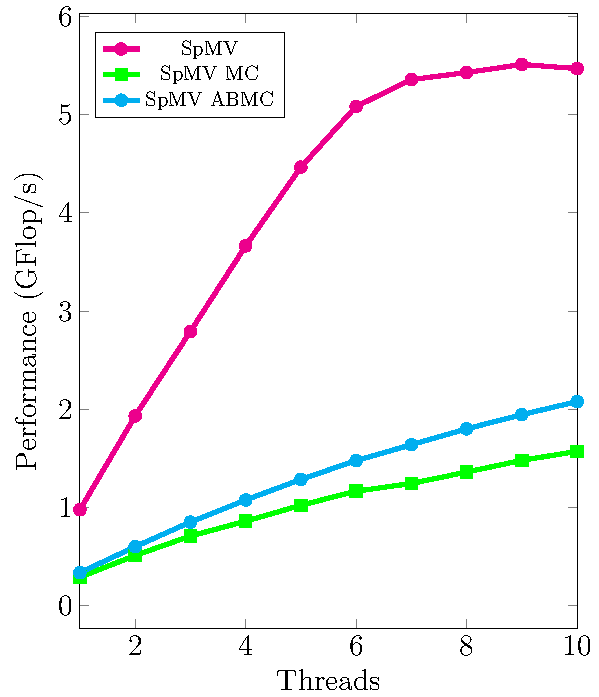
\includegraphics[width=0.26\textwidth, height=0.22\textheight]{pics/motivation/out/motivation_spmv}}
  %	\hspace{1em}
    \subfloat[SymmSpMV]{\label{fig:motivation_symm_spmv}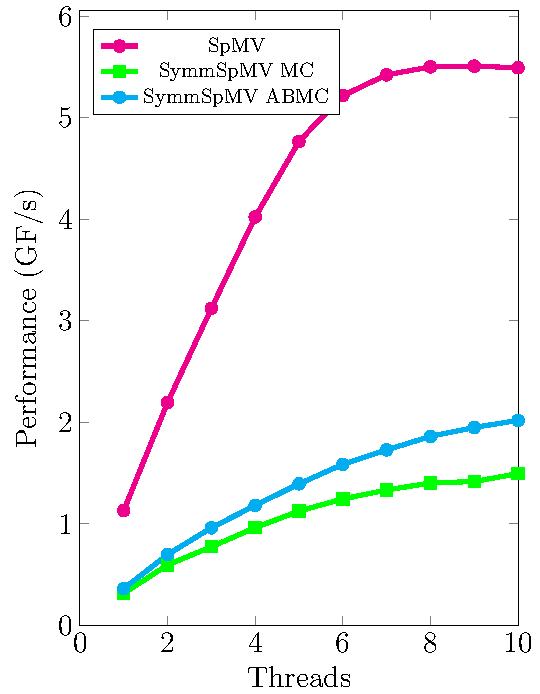
\includegraphics[width=0.38\textwidth, height=0.22\textheight]{pics/motivation/out/motivation_symm_spmv}}
    \hspace{1em}
  	\subfloat[Data Traffic]{\label{fig:motivation_data}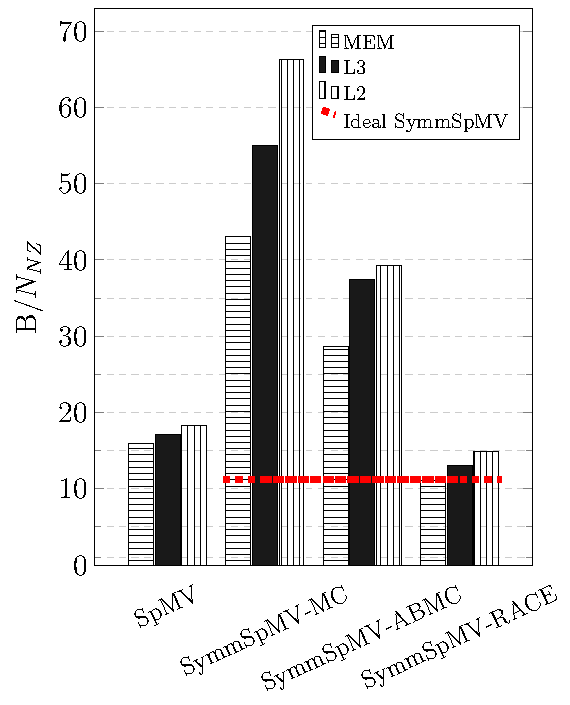
\includegraphics[width=0.4\textwidth, height=0.22\textheight]{pics/motivation/out/motivation_data_w_RACE}}
  	
  %	\subfloat[False sharing]{\label{fig:motivation_c}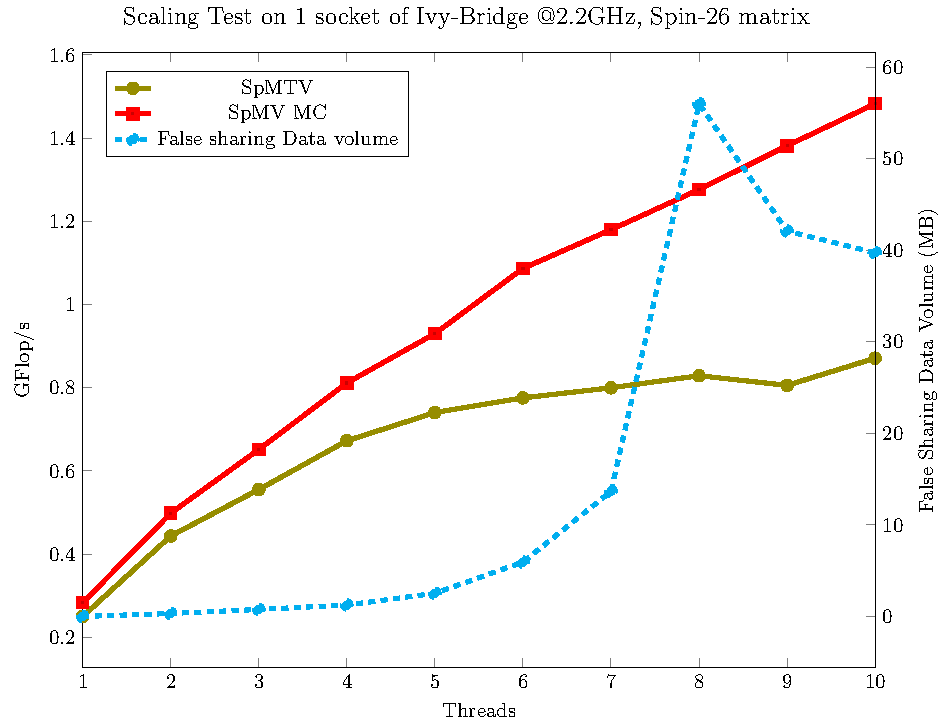
\includegraphics[width=0.45\textwidth, height=0.22\textheight]{pics/motivation/motivation_2}}
  %	\hspace{1em}
  %	\subfloat[Barrier effect]{\label{fig:motivation_d}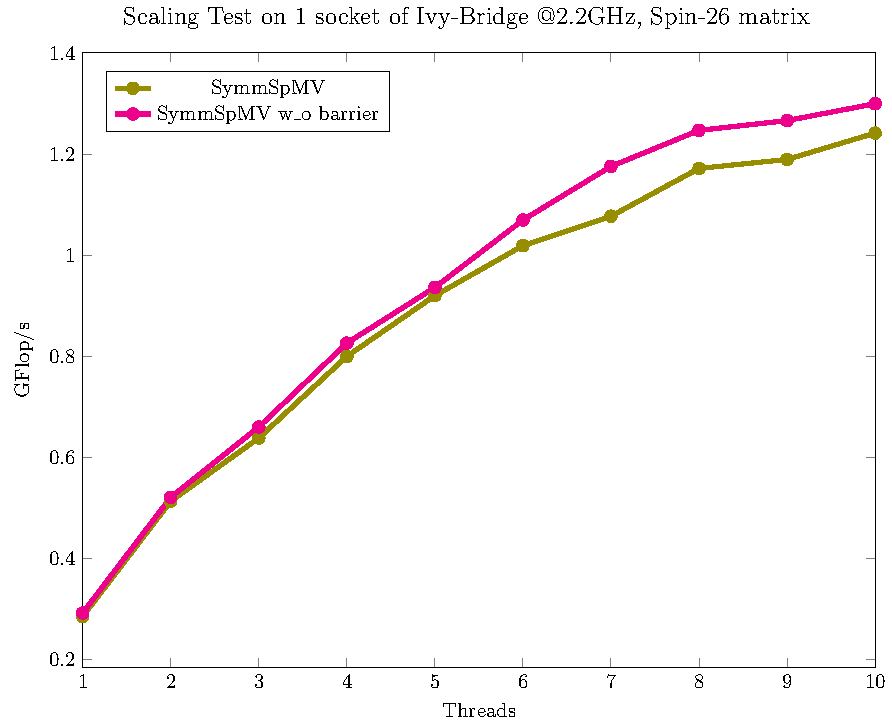
\includegraphics[width=0.45\textwidth, height=0.22\textheight]{pics/motivation/motivation_4}}
  	\caption{\Cref{fig:motivation_symm_spmv} performance of \SymmSpmv with \MC and \ABMC compared to \SpMV performance, \cref{fig:motivation_data} average data traffic per non-zero entry ($\NNZRmath$) of the full matrix as measured with \LIKWID for all cache levels and main memory. Note that all the measurements were done on \IVB socket at 2.2GHz. For all the methods matrix was pre-permuted with \RCM }
  	\label{fig:motivation}
  \end{figure}
 
\begin{comment}
{\GW Original Text - bitte auskommentieren
Motivation for developing an alternative method stems from the ESSEX (Equipping Sparse Solvers for Exascale) project \cite{ESSEX}
 where we investigate into solving large eigen-value problems from quantum mechanics field. In this context having a robust iterative solver was inevitable, due to the poor condition number of the matrices that appear in this field. Kaczmarz (\KACZ) solver was found to be satisfactory but parallelizing this solver was deemed challenging because of the loop-carried dependencies in the kernel. Previous work on parallelizing the \KACZ kernel used \MCfull (\MC) \cite{feast_mc} but it was soon found that the kernels do not scale efficiently with this approach.
In order to get a better understanding of the underlying problem it's convenient to choose simple symmetric sparse matrix vector (\SymmSpmv) as a benchmark kernel. The particular choice of this kernel is due to the fact that both \KACZ and \SymmSpmv have similar kind of dependencies, and it's much easier to compare with our reference kernel namely sparse matrix vector (\SpMV) which is embarrassingly parallel. The algorithm for \SymmSpmv  and \SpMV has been listed in \cref{alg:SymmSpMV,alg:SpMV}}
 \Cref{fig:motivation_spmv} shows the performance of \SpMV kernel on original unpermuted matrix and matrix with \MC permutation. Here we see the performance of \SpMV on multicolored matrix is  four times  worse than that of  \SpMV on unpermuted matrix. One of the major reason for this drop is due to the increase in $\alpha$ factor seen in the intensity equation \cref{eq:SpMV_intensity}  Since the kernels like \SpMV  are mainly memory bound increase in $\alpha$ lowers intensity $I_\mathrm{\SpMV}$ leading to a drop of performance as predicted by \roofline model \cite{Williams_roofline}. This could easily be demonstrated by measuring the data traffic between different memory hierarchies.  We do this using the \LIKWID tool \cite{LIKWID}, and the measurements can be seen in \cref{fig:motivation_data}. One can see an increase in data-traffic from all the memory hierarchy compared to \SpMV on normal unpermuted matrix. This is basically caused by the bad data locality introduced by \MCfull permutation.
\end{comment}
%  \begin{figure}[htbp]
 % 	\centering
  %	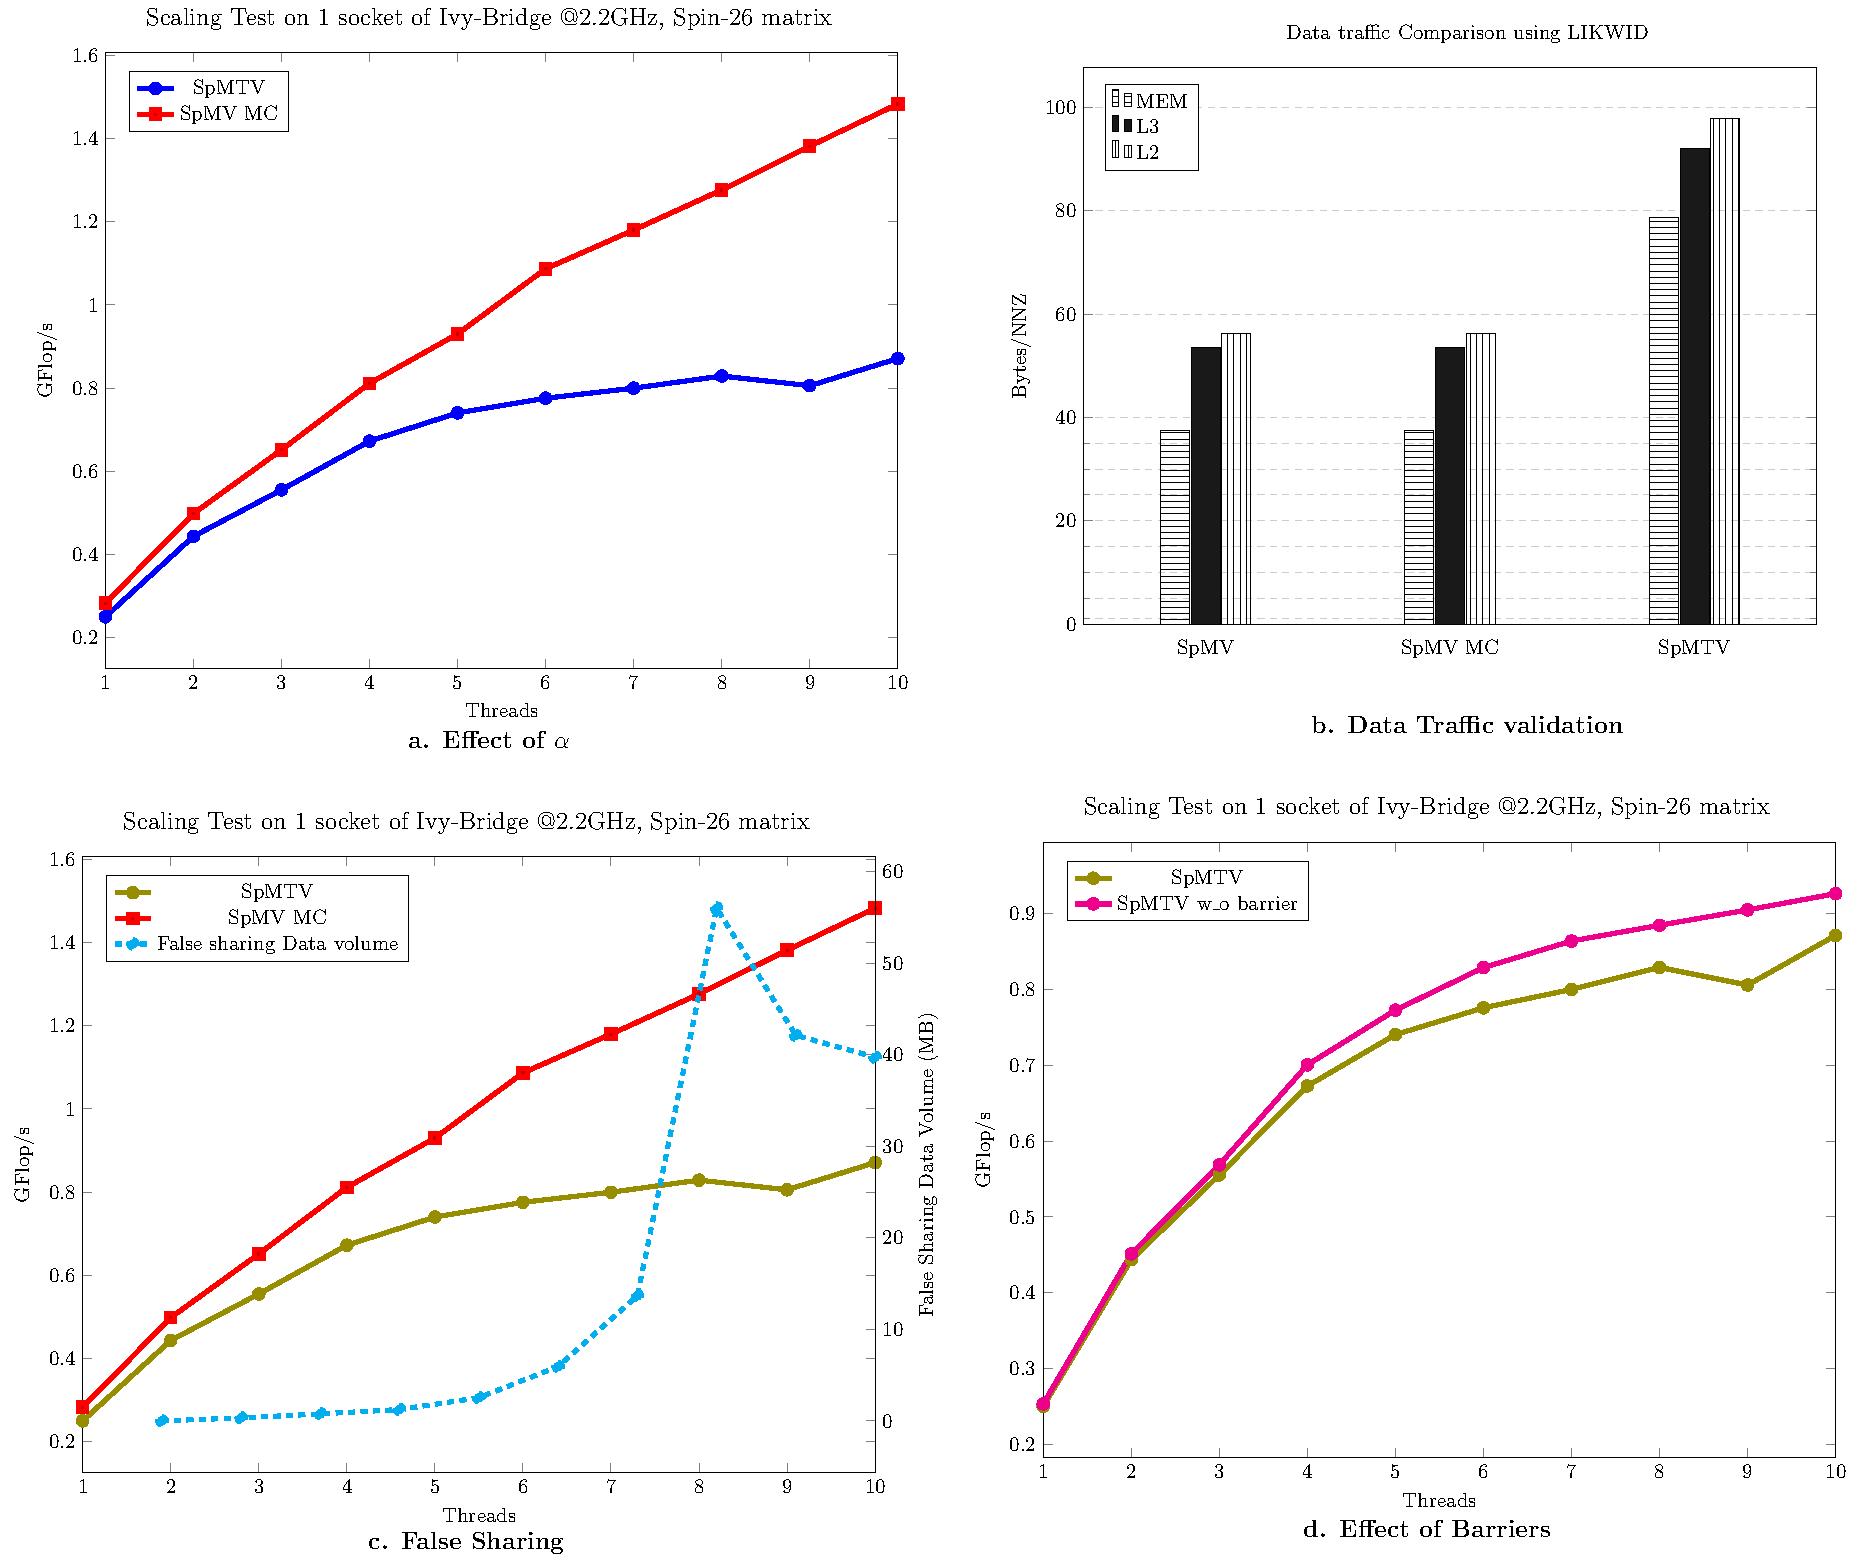
\includegraphics[width=0.9\textwidth, height=0.4\textheight]{pics/motivation/motivation}
  %	\caption{Illustration of increase in $\alpha$ by multicoloring, numbers represents thread numbers working on a particular row}
  %	\label{fig:motivation}
  %\end{figure}
  \begin{figure}[htbp]
  	\centering
  	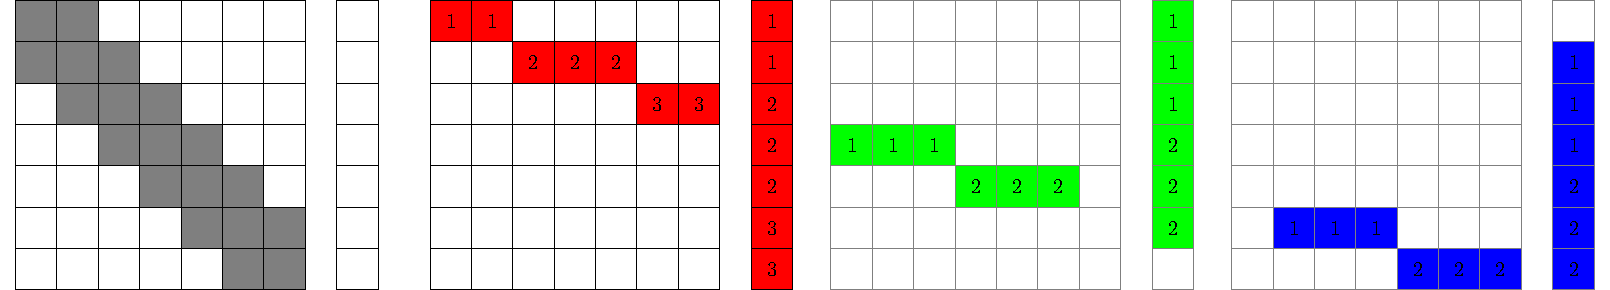
\includegraphics[scale=0.45]{pics/mc_alpha_problem/mc_alpha_unsymm}
  	\caption{Illustration of increase in $\alpha$ by multicoloring, numbers represents thread numbers working on a particular row. Please note that \cref{fig:mc_alpha} shows only rows of the matrix permuted according to \MCfull but in actual practice one would do this permutation symmetrically \ie both rows and columns are permuted.}
  	\label{fig:mc_alpha}
  \end{figure}
  
  The basic reason for this is the nature of \MCfull (\MC) permutation. For \DTWO \MC one needs  to determine sets of structurally orthogonal rows \cite{dist_k_def}, \ie rows that do not overlap in any column entry and assign different color to each set. \Cref{fig:mc_alpha} shows corresponding permutation applied to a toy problem with high data locality and the obtained sets of colors. Rows within a color can be executed in parallel but each colors are operated one after the other. As seen a color may contain rows from very different parts of the matrix potentially destroying data locality of the original matrix.  Assuming last level cache (\LLC) can hold a maximum of six elements we find for every new color we need to load right hand side vector every time for each new color. Due to this we see observe in~\cref{fig:motivation_data} we need 3$\times$ more bytes per \nnz for \SymmSpmv with \MC compared to \SpMV, although our performance model indicates we need only 0.73$\times$ that of \SpMV. Of course it is obvious this effect strongly depends on matrix structure, matrix size and cache size. 
      
  
  Algebraic Block \MCfull (\ABMC) tries to preserve data locality by first partitioning the entire matrix to blocks of specified size and then applying \MCfull to these blocks. Here we use \METIS \cite{METIS} to partition the matrix into blocks as seen in \cite{Park_HPCG}. Threads then work in parallel between blocks of the same color. This reduces data traffic as seen in \cref{fig:motivation_data} since within each blocks now we have better data locality, consequently the performance improves over \MC method (see \cref{fig:motivation_symm_spmv}). But still we do not reach near the performance model prediction of 8~\GF.
  
  One could further observe that apart from data locality other factors like global synchronizations and false sharing also contribute to the performance drops. These factors strongly depend on the number of colors and in general increase with chromatic number. For the Spin matrix the overhead of synchronization is roughly 10\% for \MC method.  For most of the matrices one could also observe a strong positive correlation between false sharing and number of threads for \SymmSpmv kernels, due to the indirect writes in \SymmSpmv.
 
 %As seen in \cref{fig:motivation_data} the data traffic further increases for \SymmSpmv, although ideally one would expect only half the data traffic as \SpMV since we operate only with upper triangle part of the matrix. The reason for this extra traffic is due to additional indirect writes (scatter) and this scales up $\alpha$ factor as seen in the denominator of $I_{\SymmSpmv}$ (see \cref{eq:SymmSpMV_intensity}),  which further decreases performance of \SymmSpmv compared to \SpMV on \MC matrix. Note that ideal performance of \SymmSpmv is almost twice as that of \SpMV if the code could saturate the memory bandwidth.
 


Overall for all the matrix in our test-suite it was seen that average drop in performance by \MCfull was almost a factor of two on a single socket of \IVB. Although for most of them performance could be improved by \ABMCfull (\ABMC), still the results we obtained were not optimal (especially for large matrices) when compared to performance models which we will see later in \cref{Sec:expt}. This led to the development of a method which works on a common data format like \CRS in which most of the other kernels are written and at the same time preserves data locality, reduce synchronization overheads and false sharing. 

With this new method called \RACE we were able to reach close to the predicted performance for most of the matrices. The performance obtained for Spin-26 matrix is shown in \cref{fig:motivation_symm_spmv}, where we achieve 7.3 \GF (91 \% of our performance model).
 



\section{Recursive Algebraic Coloring Engine (RACE)}
\label{Sec:race}
% SIAM Shared Information Template
% This is information that is shared between the main document and any
% supplement. If no supplement is required, then this information can
% be included directly in the main document.
%Keeping in mind the observations from previous \Cref{Sec:motivation}, one can observe that it would be best to maintain the nonzeros of matrix close to the diagonal.

%%Improving data locality for sparse matrix computations
%%like \acrshort{SpMV} often requires bandwidth reduction via
%%pre-processing algorithms such
%%as \acrfull{RCM} \cite{RCM,RCM_Sparse_computation}. In RACE, we thus
%%start with a bandwidth reduction approach and then apply a
%%locality-conserving coloring scheme, recursively if necessary to
%%obtain a sufficient level of parallelism. The recursion is designed
%%to avoid global synchronization between threads.
%Here, we aim to develop a method that does not distort this ideal permutations to a large extent and at the same time resolves \DK dependencies. 
Our advanced coloring algorithm is based on three steps:
\begin{enumerate}
	\item level construction,
	\item \DK coloring,
	\item load balancing.
\end{enumerate}
In the first step we apply a bandwidth reduction algorithm
including level construction and matrix reordering. We then use the
information from the level construction step to form subsets of levels
which allow for hardware efficient \DK coloring of the graph. Finally
we present a concept to ensure load balancing between threads. These steps
are applied recursively if required.


%The method is strongly coupled to the hardware underneath and exploits only the parallelism as required by the hardware. If at the end of all these four steps one does not achieve sufficient parallelism, all the steps are recursively applied to selected sub-graphs of the matrix until sufficient parallelism is attained. Due to this recursive nature of our coloring method we cal it as ``\RACfullNoSpace" (\RAC).

To illustrate the method we choose a
simple matrix which is associated with an artificially constructed
two-dimensional stencil as shown in \Cref{fig:2d-7pt-a}. The
corresponding sparsity pattern and the graph of the matrix are shown
in \Cref{fig:2d-7pt-b,fig:2d-7pt-c} respectively.
\begin{figure}[t]
	\centering
	\subfloat[\Stex]{\label{fig:2d-7pt-a}
\includegraphics[width=0.17\textwidth , height=0.13\textheight]{pics/2d-7pt/stencil.pdf}}
	\hspace{0.8em}
	\subfloat[Sparsity
	 pattern]{\label{fig:2d-7pt-b}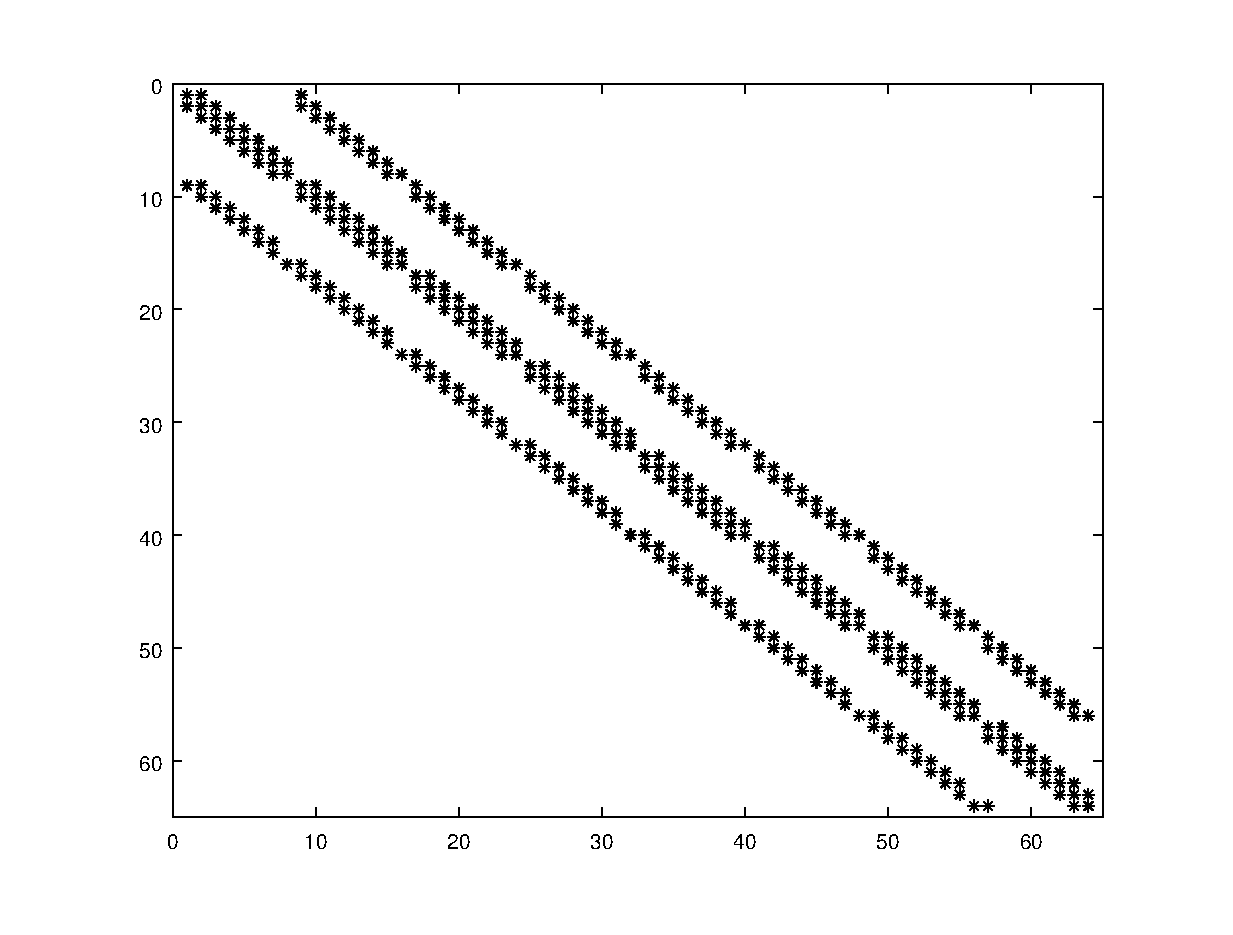
\includegraphics[width=0.38\textwidth , height=0.19\textheight]{pics/2d-7pt/2d_7pt_bw.eps}}
	\hspace{1em}
	\subfloat[Graph]{\label{fig:2d-7pt-c}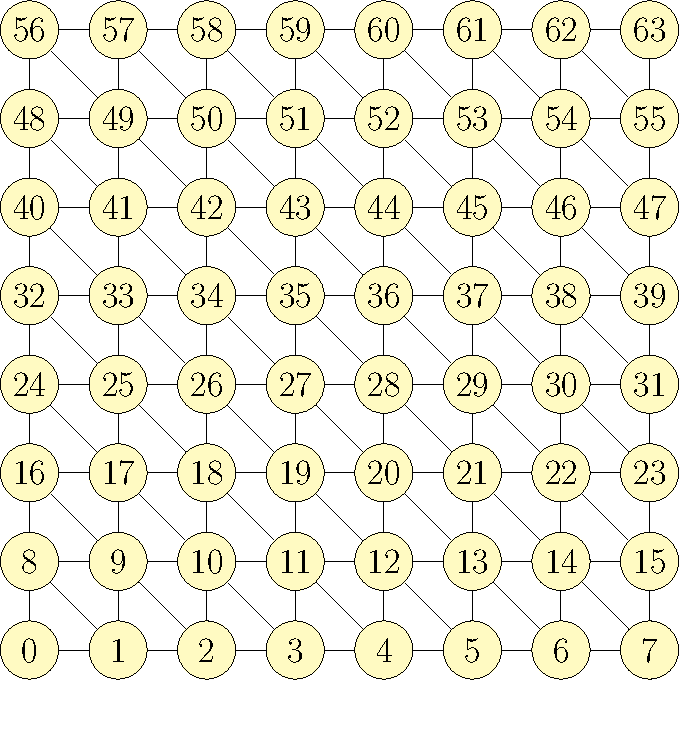
\includegraphics[width=0.3\textwidth , height=0.18\textheight]{pics/2d-7pt/stencil_2d_7pt.pdf}}
	\caption{\sref{fig:2d-7pt-a} Structure of an artificially designed stencil,
	\sref{fig:2d-7pt-b} corresponding sparsity pattern of its matrix
	representation on an $8\times 8$ lattice with Dirichlet
	boundary conditions, and \sref{fig:2d-7pt-c} the graph representation of the
	matrix. The stencil
	structure was chosen for illustration purposes and does not
	represent any specific application scenario.}
	\label{fig:2d-7pt}
\end{figure}

\subsection*{Definitions}
We need the following definitions from graph theory:
\begin{itemize}
	\item \textbf{Graph: } $G = (V,E)$ represents a graph, with $V(G)$
              denoting its set of vertices and $E(G)$ denoting its edges. Note that
              we restrict ourselves to irreducible undirected graphs.
	\item \textbf{Neighborhood:} $N(u)$ is the neighborhood of a vertex $u$ and is defined as
	\begin{equation*}
	  N(u) = \set{ v \in V(G) : (u,v) \in E(G)}\eos
	 %N(u) = { v \in V(G) : (u,v) \in E(G)}
	\end{equation*}
	\item \textbf{$k$th Neighborhood:} $N^{k}(u)$ of a vertex $u$ is defined as
	 \begin{align*}
	 	N^2(u) &= N(N(u))  \\
	 	N^3(u) &= N^2(N(u)) \\
	 	\vdots\\
	 	N^k(u) &= N^{k-1}(N(u)) \eos
	 \end{align*}
	\item \textbf{Subgraph:} In this paper a subgraph $H$ of $G$ specifically
              refers to the subgraph induced by vertices $V' \subseteq V(G)$ and is defined as
	\begin{equation*}
		H = (V', \set{ (u,v) : (u,v) \in E(G) \text{ and } u,v \in V'})\eos
	\end{equation*}
\end{itemize}

\subsection{Level Construction}\label{subsec:LEVEL_CONST}

The first step of \acrshort{RACE} is to determine
different \textit{\levels} in the graph and permute the
graph data structure. This we achieve using
well-known bandwidth reduction algorithms such as \acrfull{RCM} \cite{RCM}
or \acrfull{BFS} \cite{BFS}\@. Although the RCM method is
also implemented in \acrshort{RACE}, we use the \acrshort{BFS}
reordering in the following for simpler illustration.

%\acrshort{BFS} can also be replaced with better bandwidth reduction algorithms like ``(Reverse) \CMfull".  

First we choose a \emph{root} vertex and assign it to the
first \level, $L(0)$\@. For $i>0$, \level \acrshort{L_i}
is defined to contain vertices that are in the neighborhood of vertices
in $L(i-1)$ but not in the neighborhood of vertices
in $L(i-2)$ \cite{BFS_level_def}, \ie
\begin{equation}\label{eq:level}
L(i) = 
\begin{cases}
	 root & \text{ if } i = 0, \\
	 u : u \in N(L(i-1))  & \text{ if } i = 1, \\
	 u : u \in N(L(i-1)) \cap \overline{N(L(i-2))}  & \text{otherwise}.
\end{cases}   
\end{equation}
From \Cref{eq:level} one finds that the $i$th \level consists of all
vertices that have a minimum distance $i$ from the root node.
\Cref{alg:BFS} shows how to determine this distance and thus set up the
\levels $L(i)$\@. We refer to the total number of \levels obtained for a particular graph
as \acrshort{totalLvl}. \Cref{fig:2d_7pt_level_construction} shows the
\acrshort{totalLvl}=14 \levels of our artificial stencil
operator, where the index of each vertex ($v$) is the
vertex number and the superscript represents the \level number, \ie
\begin{equation}\label{eq:node_notation}
	v^i \implies v \in L(i)\eos
\end{equation}
Note that the $L(i)$ are  substantially different from the \levels used in
the ``level-scheduling" \cite{saad} approach, which applies ``depth first
search."

\setlength{\fboxsep}{0pt}%

\begin{figure}[t]
	\centering
	\subfloat[Level construction]{\label{fig:2d_7pt_level_construction}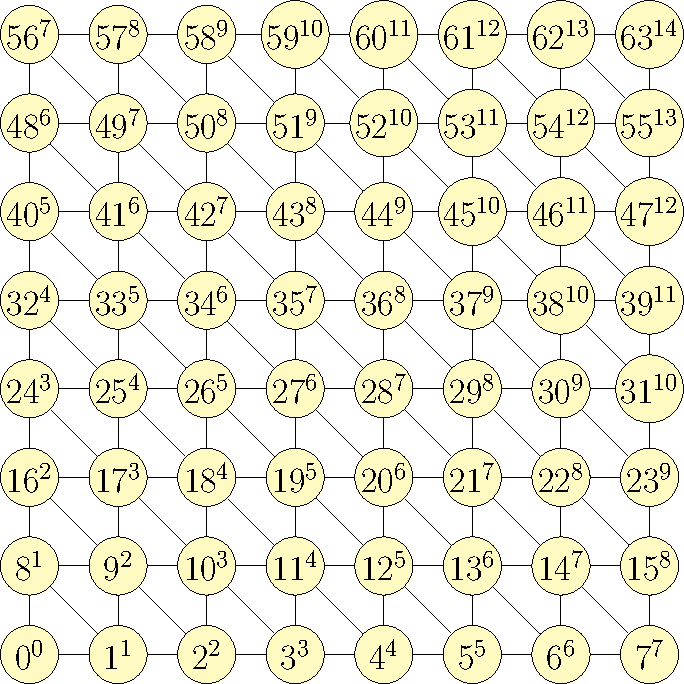
\includegraphics[height=0.18\textheight,width=0.32\textwidth]{pics/level_construction/stencil_2d_7pt}
			\begin{picture}(0,0)
			\put(-44,68){\fbox{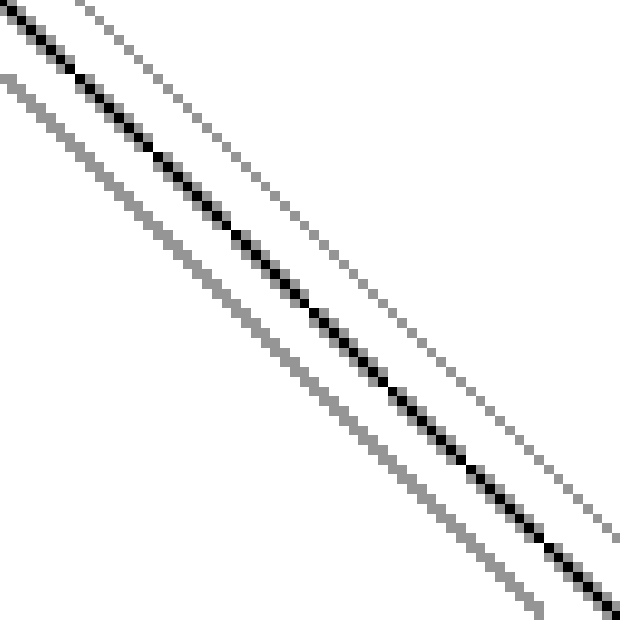
\includegraphics[height=1.4cm]{pics/level_construction/FDM_2d_7pt_non_perm}}}
			\end{picture}
		}
	\hspace{1em}
	\subfloat[Permuted graph ($G'$)]{\label{fig:2d_7pt_perm}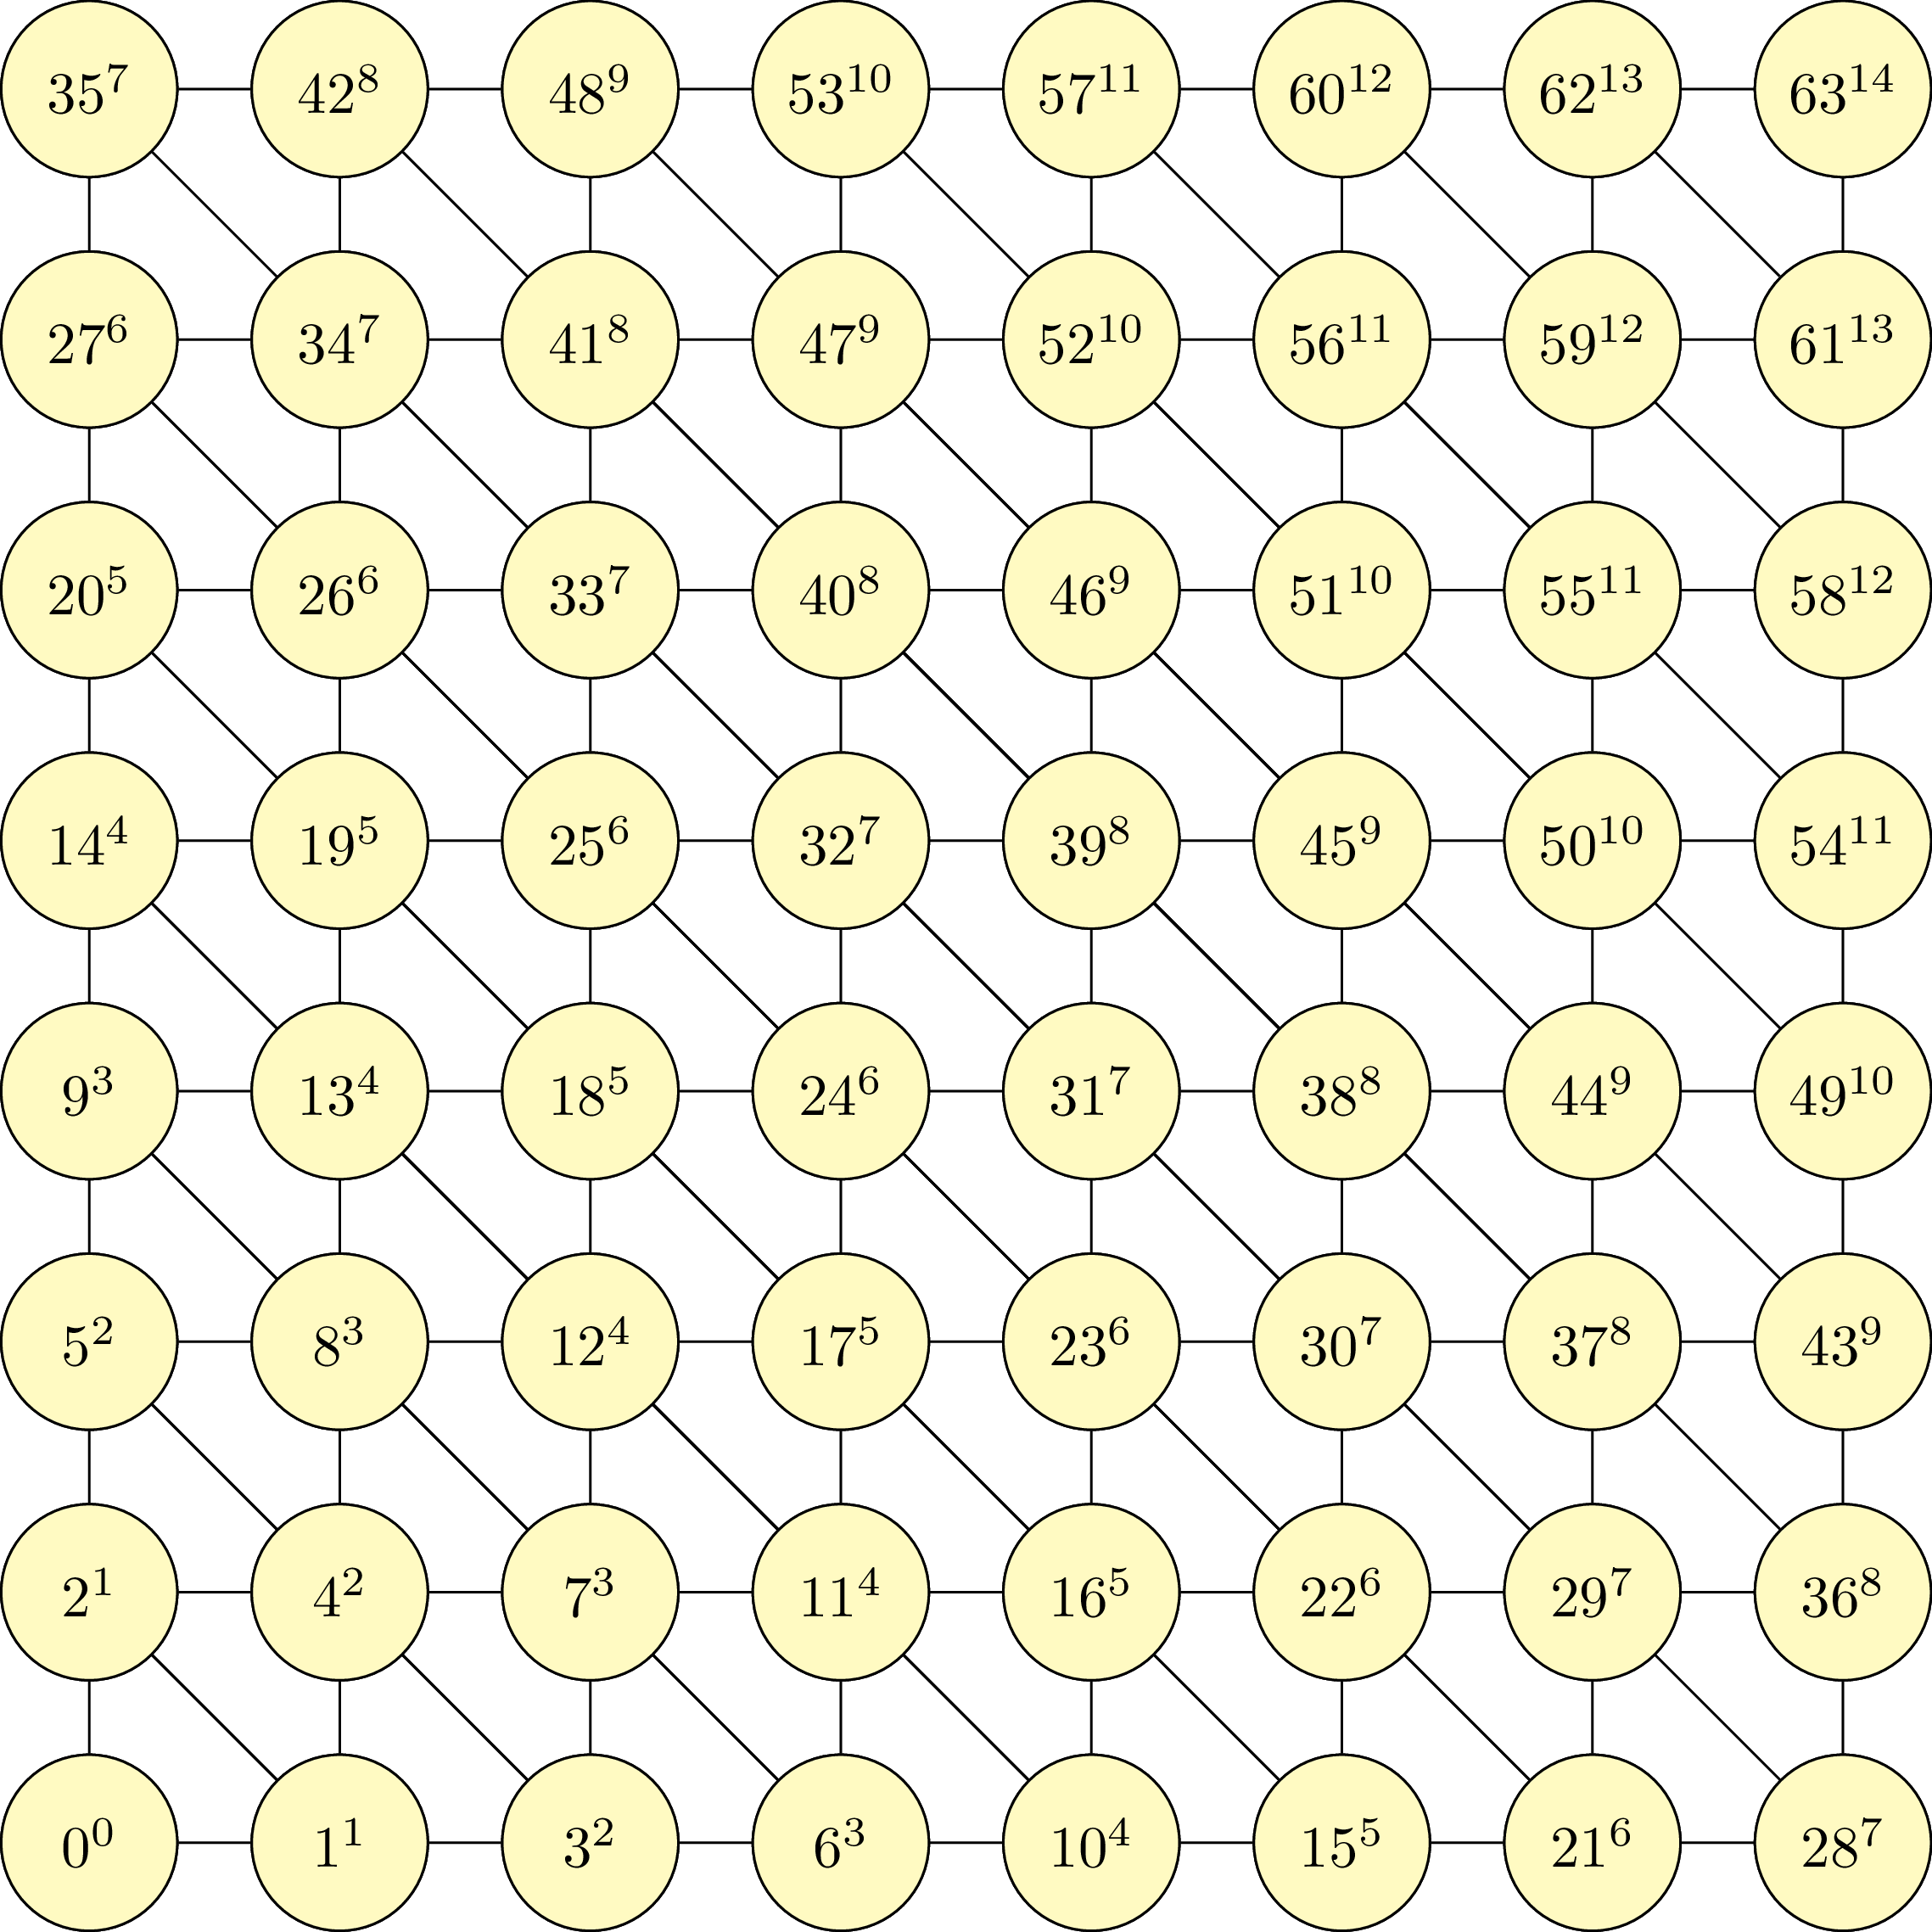
\includegraphics[height=0.18\textheight,width=0.32\textwidth]{pics/permutation/stencil_2d_7pt}
			\begin{picture}(0,0)
			\put(-43.5,68){\fbox{
\includegraphics[height=1.4cm]{pics/permutation/FDM_2d_7pt_perm}}}
			\end{picture}
		}
	\hspace{1em}
	\subfloat[]{\label{fig:2d_7pt_levelPtr}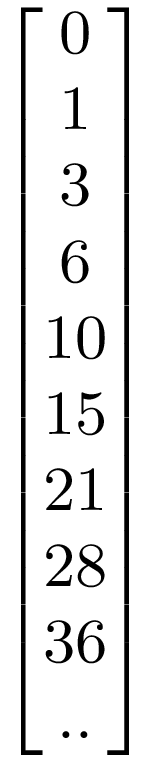
\includegraphics[height=0.18\textheight,width=0.07\textwidth]{pics/permutation/levelPtr}}
	\caption{\sref{fig:2d_7pt_level_construction} Levels of the original graph and \sref{fig:2d_7pt_perm} the permuted
          graph for the \stex. Insets show the corresponding sparsity patterns.
          \sref{fig:2d_7pt_levelPtr} Shows the entries of the \levelPtr array associated
          with $G'$.}
	\label{fig:2d-7pt_step_1_2}
\end{figure}


%\subsection{Permutation}\label{subsec:PERM}

After the \levels have been determined, the matrix is permuted in the
order of its \levels, such that the vertices in $L(i)$ are stored
consecutively and appear before those of
$L(i+1)$. \Cref{fig:2d-7pt_step_1_2} shows the graph ($G' = P(G)$)
of the \stex after applying this permutation ($P$) and demonstrates
the enhanced spatial locality of the vertices within and between
\levels (see \Cref{fig:2d_7pt_perm}) as compared to the original
(lexicographic) numbering (see \Cref{fig:2d_7pt_level_construction}).
Until now the procedure is the same as \acrshort{BFS} (or
\acrshort{RCM}).

As \acrshort{RACE} uses information about the \levels for resolving
dependencies in the coloring step, we store the index of the entry point to each
\level in the permuted data structure (of $G'$) in an array
$\levelPtr[0:$ \acrshort{totalLvl}$]$, so that \levels on $G'$ can be
identified as
\begin{equation*}
  L(i) = \set{ u : u \in [\levelPtr[i]:(\levelPtr[i+1]-1)]
    \text{ and } u \in V(G')}\eos
\end{equation*}
The entries of \levelPtr for the \stex are shown in \Cref{fig:2d_7pt_levelPtr}. 
%, and one could easily read from \levelPtr that vertices from $\levelPtr(4)=7$ to $\levelPtr(5)-1=10$ belongs to $L(4)$.
 
\subsection{Distance-k coloring} \label{subsec:DK}

The data structure generated above serves as the basis for our \DK coloring
procedure as it contains information about the neighborhood relation
between the vertices of any two \levels. Following the definition
in~\cite{dist_k_def}, two vertices are called \DK neighbors if the
shortest path connecting them consists of at most $k$ edges.
%In this section we introduce the idea of \DK neighbor and show how
%this idea can be used to color the matrix with the help of the level
%information that we already have in hand.
This implies that $u$ is a \DK neighbor of $v$ (referred to as
$u\xrightarrow{k}v$) if
\begin{equation}\label{eq:dk}
  u\xrightarrow{k}v  \iff  v \in \set{ u \cup N(u) \cup N^2(u) \cup \cdots N^k(u) }\eos
\end{equation}
For the undirected graphs as used here, $u\xrightarrow{k}v$
also implies $v\xrightarrow{k}u$. Based on this definition we consider
two vertices to be \DK independent if they are not \DK
neighbors, and two \levels are said to be \DK independent 
%if the vertices between them are \DK independent. 
if their vertices are mutually \DK independent.
Thus, \levels $L(i)$ and $L(i\pm(k+j))$ of the permuted
graph $G'$ are \DK independent for all $j\geq1$, denoted as
\begin{equation}\label{corollary_dk}
	L(i) \not{\xrightarrow{k}} L(i\pm(k+j)) \forall j\geq1 \eos
\end{equation} 

\begin{comment}
 as shown in the
following.
\begin{corollary}\label{corollary_dk}
$L(i)$ and $L(i\pm(k+j))$ are \DK independent $\forall j\geq1$. 
\end{corollary}
\begin{proof}
  We prove by contradiction. Let there exist $u,v \in V(G')$ such that
  $u \in L(i)$ and $v \in \bigcup\limits_{j\geq 1}L(i \pm (k+j))$. Assume $u,v$
  are \DK neighbors ($u\xrightarrow{k}v$). From \Cref{eq:level},
  \Cref{eq:dk}, and the fact $G'$ is undirected we get
\begin{align*}
  u\xrightarrow{k}v \iff & v \in \set{L(i) \cup L(i \pm 1) \cup \cdots \cup L(i \pm k)} \\
  \implies & v \notin L(i \pm (k+j)) \text{  } \forall j \geq 1\cma
\end{align*}
which contradicts our assumption about $v$\@.
Thus it follows that $u$ and $v$ are \DK independent.
\end{proof}
\end{comment}

\Cref{corollary_dk} implies that if there is a gap of at least
one \level between any two \levels (e.g., $L(i) \mbox{ and } L(i+2)$) all
pairs of vertices between these two levels are \DONE independent. Similarly
if the gap consists of at least two \levels between any two
\levels (e.g., $L(i) \mbox{ and } L(i+3)$) we have \DTWO independent
\levels, and so on.
 \begin{figure}[t]
 	\centering
 	\subfloat[Distance-1 independent \levelGroups]{\label{fig:2d_7pt_d1}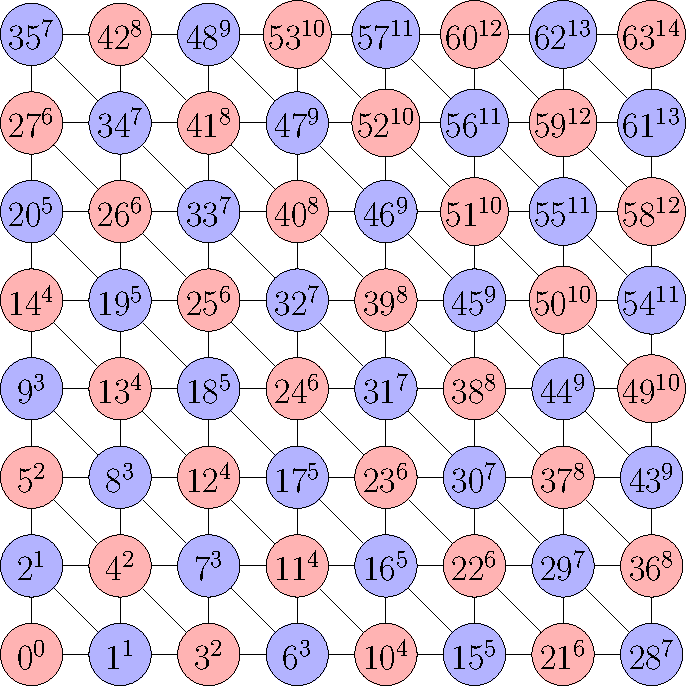
\includegraphics[height=0.2\textheight,width=0.4\textwidth]{pics/dk_coloring/stencil_2d_7pt_d1}}
 	\hspace{2.5em}
 	\subfloat[Distance-2 independent \levelGroups]{\label{fig:2d_7pt_d2}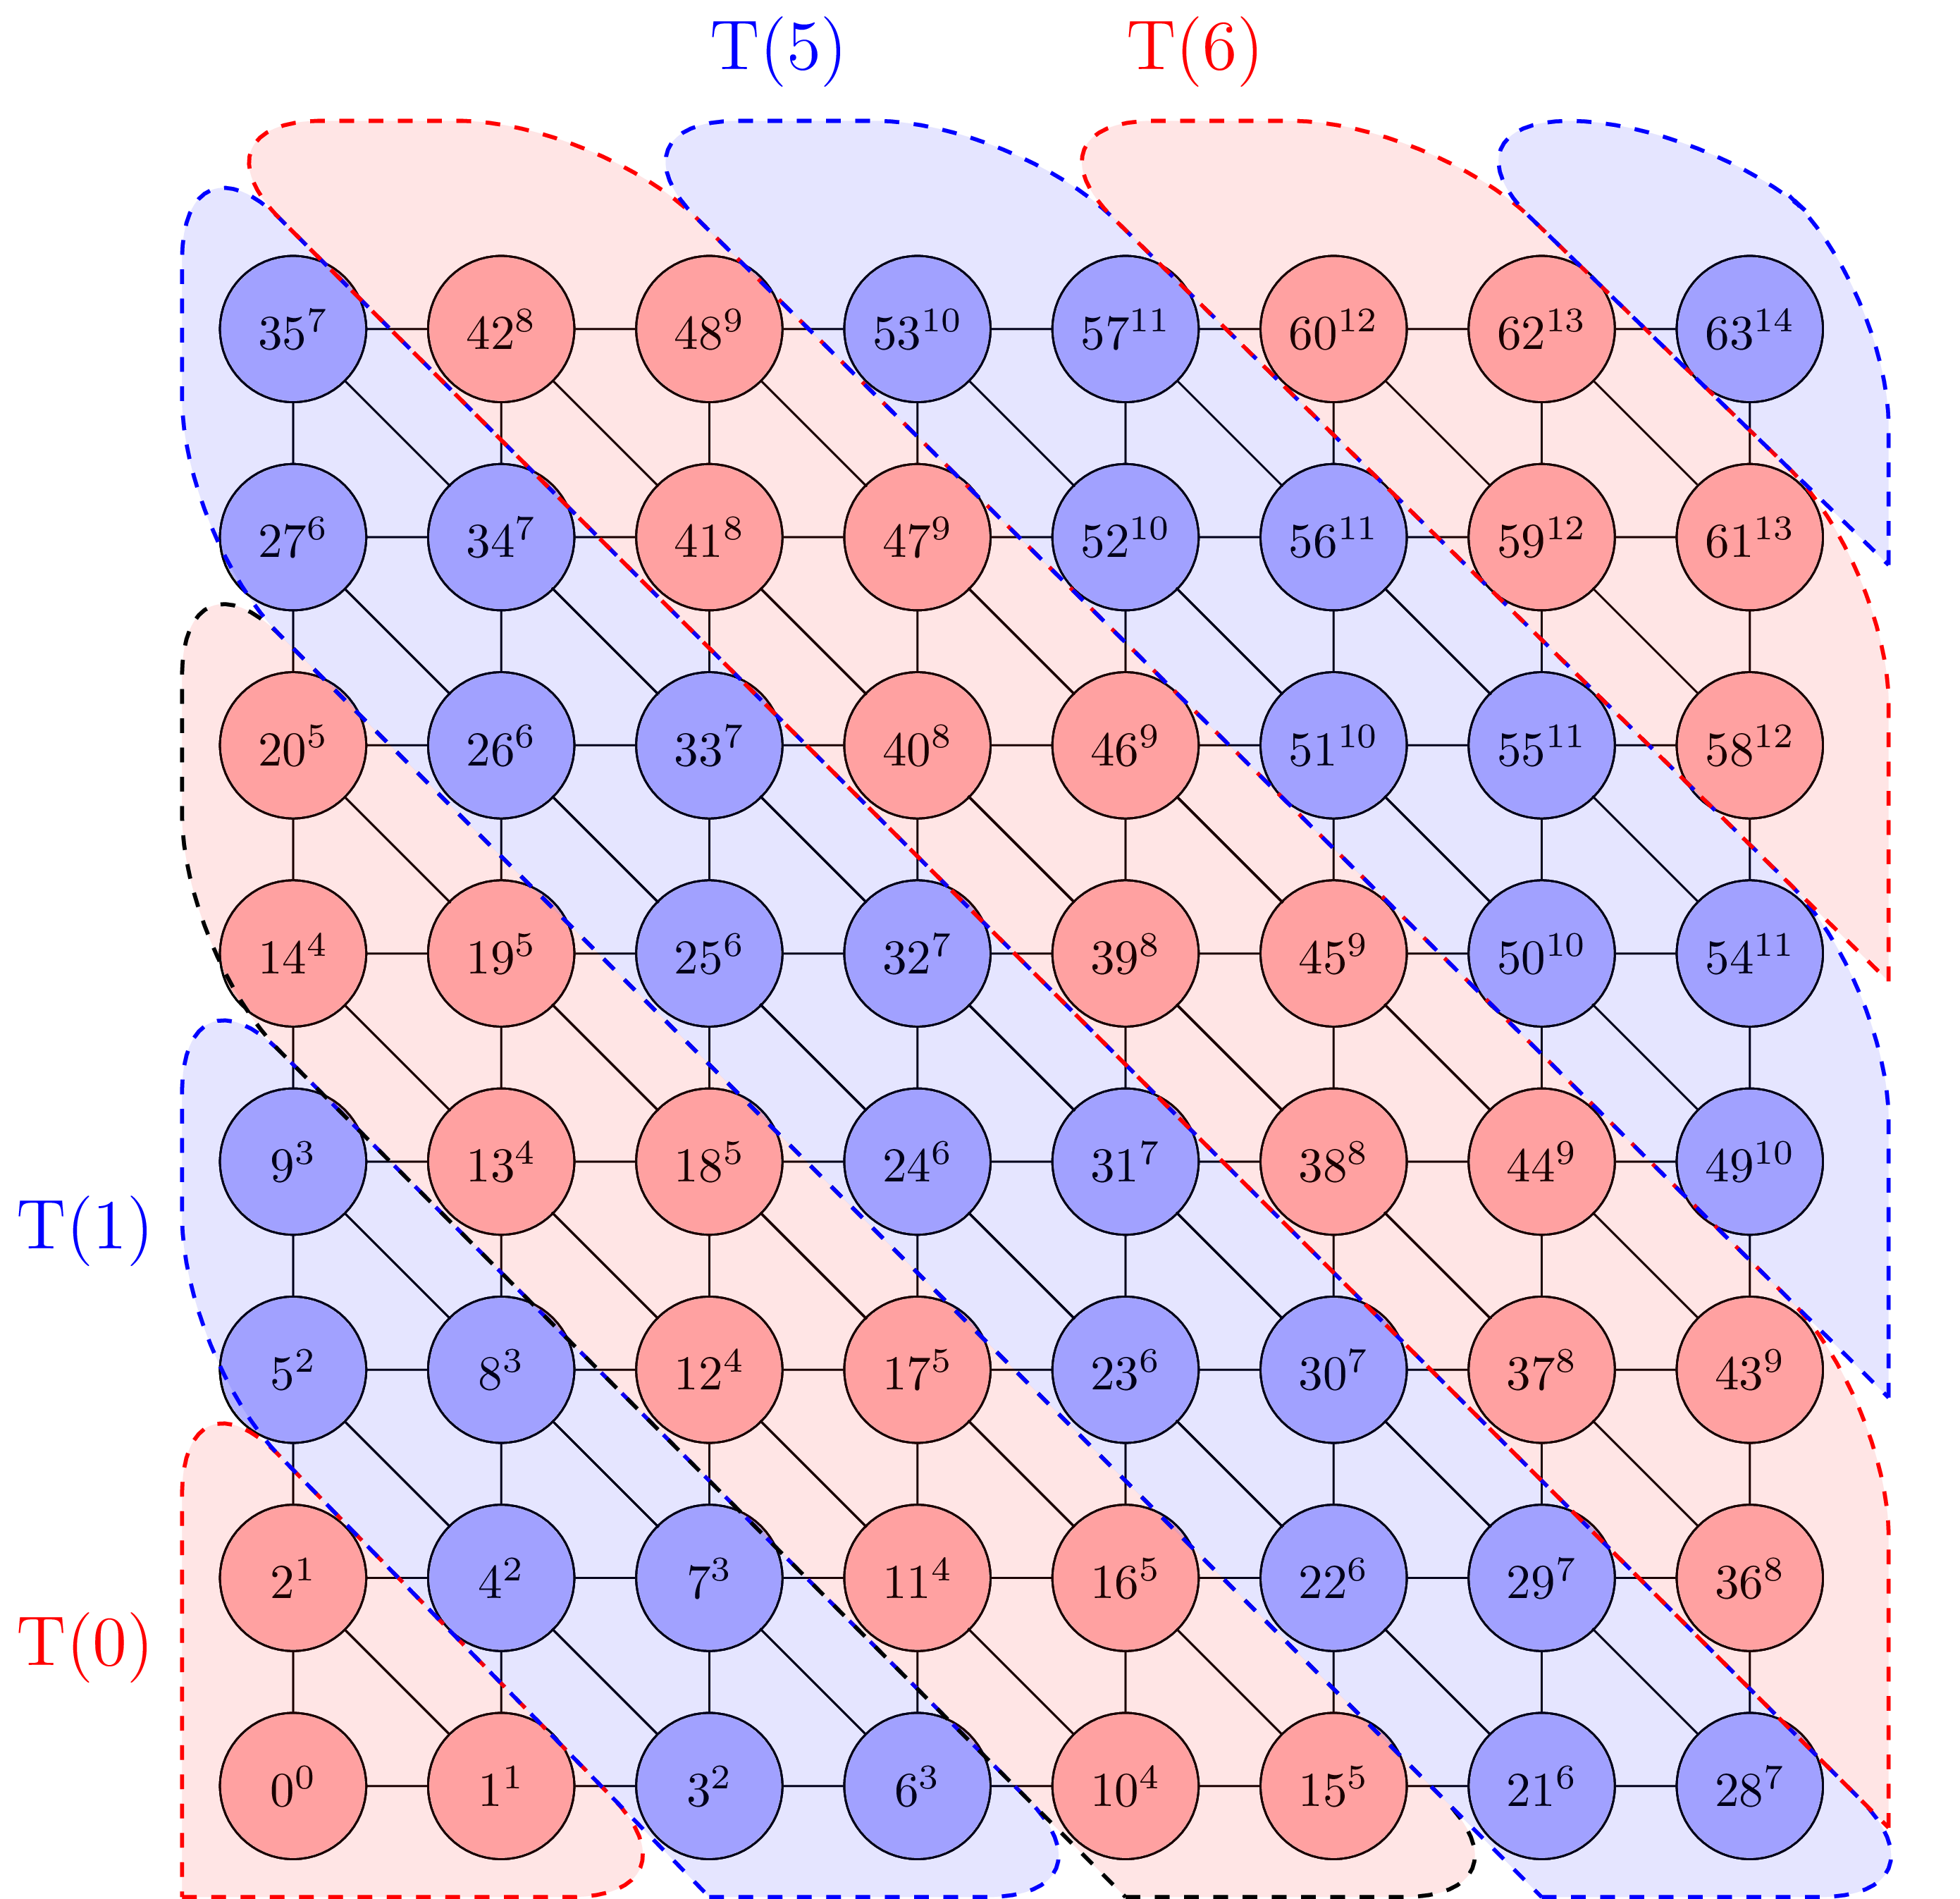
\includegraphics[height=0.23\textheight,width=0.48\textwidth]{pics/dk_coloring/stencil_2d_7pt_d2_with_lg}}
 	\caption{Forming \DONE and \DTWO independent \levelGroups for the \stex.}
 	\label{fig:2d-7pt_d1_d2}
 \end{figure}
 
 
The definition used in \Cref{corollary_dk} offers many choices for
forming \DK independent sets of vertices, which can then be executed
in parallel.  In \Cref{fig:2d-7pt_d1_d2} we present one example each
for \DONE (\Cref{fig:2d_7pt_d1}) and \DTWO (\Cref{fig:2d_7pt_d2})
colorings of our \stex. The \DONE coloring uses a straightforward
approach by assigning two colors to alternating \levels, i.e., \levels
of a color can be calculated concurrently. In case of \DTWO
independence we do not use three colors but rather aggregate two
adjacent \levels to form a \textit{\levelGroup} (denoted by
\acrshort{T_i}) and perform a \DONE coloring on top of those
groups. This guarantees that vertices of two \levelGroups of the same
color are \DTWO independent and can be executed in parallel. Here, the
vertices in $T(0)$, $T(2)$, $T(4)$, and $T(6)$ can be operated on by
four threads in parallel, i.e., one thread per \levelGroup.  After
synchronization the remaining four blue \levelGroups can also be
executed in parallel. This idea can be generalized such that for \DK
coloring, each \levelGroup contains $k$ adjacent \levels.
%\atleast $k$ adjacent \levels but
%the number of \levels  per \levelGroup may be different. 
Thus formed \levelGroups are then \DONE
colored. Then, all \levelGroups within a color can be executed in
parallel. This simple approach allows one to generate workload for
a maximum of ${\acrshort{totalLvl}}/{2 k}$ threads if \DK coloring is
requested. \footnote{\CAcomm{This implies more the number of levels more the
parallelism, for \eg if the matrix contains at least one row that
is fully dense (row with \acrshort{nrows} nonzeros) it will have no parallelism, 
as $\acrshort{totalLvl}=2$ in this case.}} Note that in all cases vertices within a single \levelGroup
 are computed in their original order, which allows for good
spatial access locality.
 
Choosing the same number of \levels for each \levelGroup may
however cause severe load imbalance depending on the matrix structure. In
particular the use of bandwidth reduction schemes such as BFS or RCM
will further worsen that problem due to the lenslike shape of the
reordered matrix (see inset of \Cref{fig:2d_7pt_perm}), leading to low
workload for \levelGroups containing the top and bottom rows of the
  matrix. Compare, \eg $T(0)$ and $T(7)$ with $T(3)$ and $T(4)$ in
\Cref{fig:2d_7pt_d2}. However, \Cref{corollary_dk} does not require
exactly $k$ levels to be in a \levelGroup but  
requires only ``\atleast'' k \levels in a \levelGroup. In
the following we exploit this to alleviate the imbalance
problem.
 %coloring by aggregating consecutive levels into \levelGroups (denoted by $T(i)$). In  \Cref{fig:2d_7pt_d1}  and \Cref{fig:2d_7pt_d2} we present one example for \DONE and \DTWO coloring of our \stex, respectively. The \DONE coloring uses straight forward approach by assigning two colors to alternating levels, i.e. \levelGroup and \level is equivalent here. For and applying a \DONE coloring on top of those groups as shown for \DTWO coloring in \Cref{fig:2d_7pt_d2}.  In this context \Cref{fig:2d-7pt_d1_d2} contains two potential colorings for \DONE independent \levels as \DTWO coloring also solves \DONE dependencies.  One could also group some more of nearby \levels together to form a \levelGroup, and make this \DONE or \DTWO independent of other \levelGroups. The $i$-th \levelGroup would be denoted by $T(i)$. Difference between \level and  \levelGroup can be seen in \Cref{fig:2d_7pt_d2}, for \Cref{fig:2d_7pt_d1} \levelGroup and \level coincides. In principle one could compute on all independent \levelGroups in parallel, but sequentially within a \levelGroup, \ie for example in \Cref{fig:2d_7pt_d2} $T(0)$, $T(2)$, $T(4)$, $T(6)$ can be operated by four different threads in parallel and in the next sweep rest \levelGroups. For the configurations seen in \Cref{fig:2d-7pt_d1_d2} then we have $\frac{\acrshort{totalLvl}}{2}$ and $\frac{\acrshort{totalLvl}}{4}$ parallelism for \DONE and \DTWO kernels respectively.
 %However the problem with the configurations like the one seen in \Cref{fig:2d-7pt_d1_d2} {\CA is that there, check Holger's comment} is load imbalances between threads because the number of rows (\nrows) per \levelGroup is not distributed evenly. As seen here in the case of \stex the threads working on extreme ends of graph (\eg $T(1), T(7)$) have a small amount of work compared to the threads working on middle (\eg $T(3), T(4)$). 
  
  \subsection{Load balancing}\label{subsec:LB} 
The RACE load balancing scheme tries to balance the workload between level groups 
within each color for a given number of threads while maintaining data locality 
and \DK constraint between the two colors. \CAcomm{To achieve this we use an idea
similar to incremental graph partitioning \cite{load_balancing}}. 
The \levelGroups containing low workload grab adjacent levels from neighboring
 level groups and overloaded level groups shift levels to adjacent level groups. 
 As a target for the load balancing scheme one can balance the number of rows (\ie vertices) 
 of the \levelGroups ($\acrshort{nrows}(T(i))$)  or the number of nonzeros (\ie edges) of the 
 \levelGroups ($\acrshort{nnz}(T(i))$). Both variants are supported by our implementation 
 and we choose balancing by the number of rows in the following to demonstrate our load 
 balancing algorithm, which can be found in \Cref{alg:LB}.
%Depending on the matrix each \levelGroup contains different number of rows, that leads to load imbalances as seen above in \Cref{subsec:DK}. \Inorder to avoid this problem we employ a load balancing scheme. At this step  we plug in details from the hardware side  namely the total parallelism required by the hardware. The idea is to exploit only the required parallelism while at the same time maintain \DK constraint seen in \Cref{corollary_dk}. To balance the load more nearby \levels would be added to a \levelGroup ($T(x)$) which has less number of rows ($\nrowsMath(T(x))$) and at \levelGroup where we have considerably big \levels only sufficient amount of \levels to maintain \DK constraint would be assigned. Assigning nearby levels instead of others further helps in preserving data locality. 
 
Our algorithm tries to reduce the variances of the workload in the level groups, \ie the number of rows ($\acrshort{nrows}(T(i))$) in each \levelGroup $T(i)$. For a given set of \levelGroups we calculate the mean and variance of $\acrshort{nrows}(T(i))$ within each color, \ie red and blue colors.  
 %For example in \Cref{fig:2d_7pt_d2} we need to calculate mean of $T\_size$ of all \levelGroups in red sweep and blue sweep separately. 
The overall variance, which is the target of our minimization procedure, is then found by summing up the variances between colors. \Inorder to reduce this value we first select the two \levelGroups with largest negative/positive deviation from the mean \CAcomm{(in step 1 of \Cref{fig:lb_alg} $T(5)$ and $T(4)$)} and try to add/remove levels to/from these \levelGroups (see top row of \Cref{fig:lb_alg}). When removing \levels from a \levelGroup one has to take care that the \DK coloring is not violated by keeping at least $k$ levels in a \levelGroup. The shift of \levels is done via a pointer array denoted as $T\_ptr$, which points to the beginning of each \levelGroup (see \Cref{fig:lb_alg}), avoiding any copy operation. If shifting levels between the two level groups with the largest deviation does not lead to a lower overall variance, no levels are exchanged and we choose the next pair of level groups according to a ranking which is based on the absolute deviation from the mean (see \Cref{alg:LB} for implementation details) and continue. Doing this process in an iterative way we finally end up in a state with the lowest overall variance at which no further moves are possible either due to a violation of \DK dependency or an increase in overall variance. \Cref{fig:lb_alg} shows the load balancing procedure under a \DTWO constraint for some initial mapping of 17 levels to six level groups. Applying the procedure to our  \stex of size $16 \times 16$  requesting \DTWO coloring and ten level groups leads to the mapping shown in \Cref{fig:2d_7pt_lb}. Note that \levelGroups at the extreme ends have more \levels due to fewer vertices (\acrshort{nrows}) in each \level, while \levelGroups in the middle having more vertices maintain two levels to preserve the \DTWO constraint.
%One could also do this entire load balancing based on number of nonzeros (\acrshort{nnz}) rather than \nrows, in this case $T\_size(i)=\acrshort{nnz}(T(i))$ (nonzeros in $T(i)$).
  
   \begin{figure}[t]
   	\centering
   	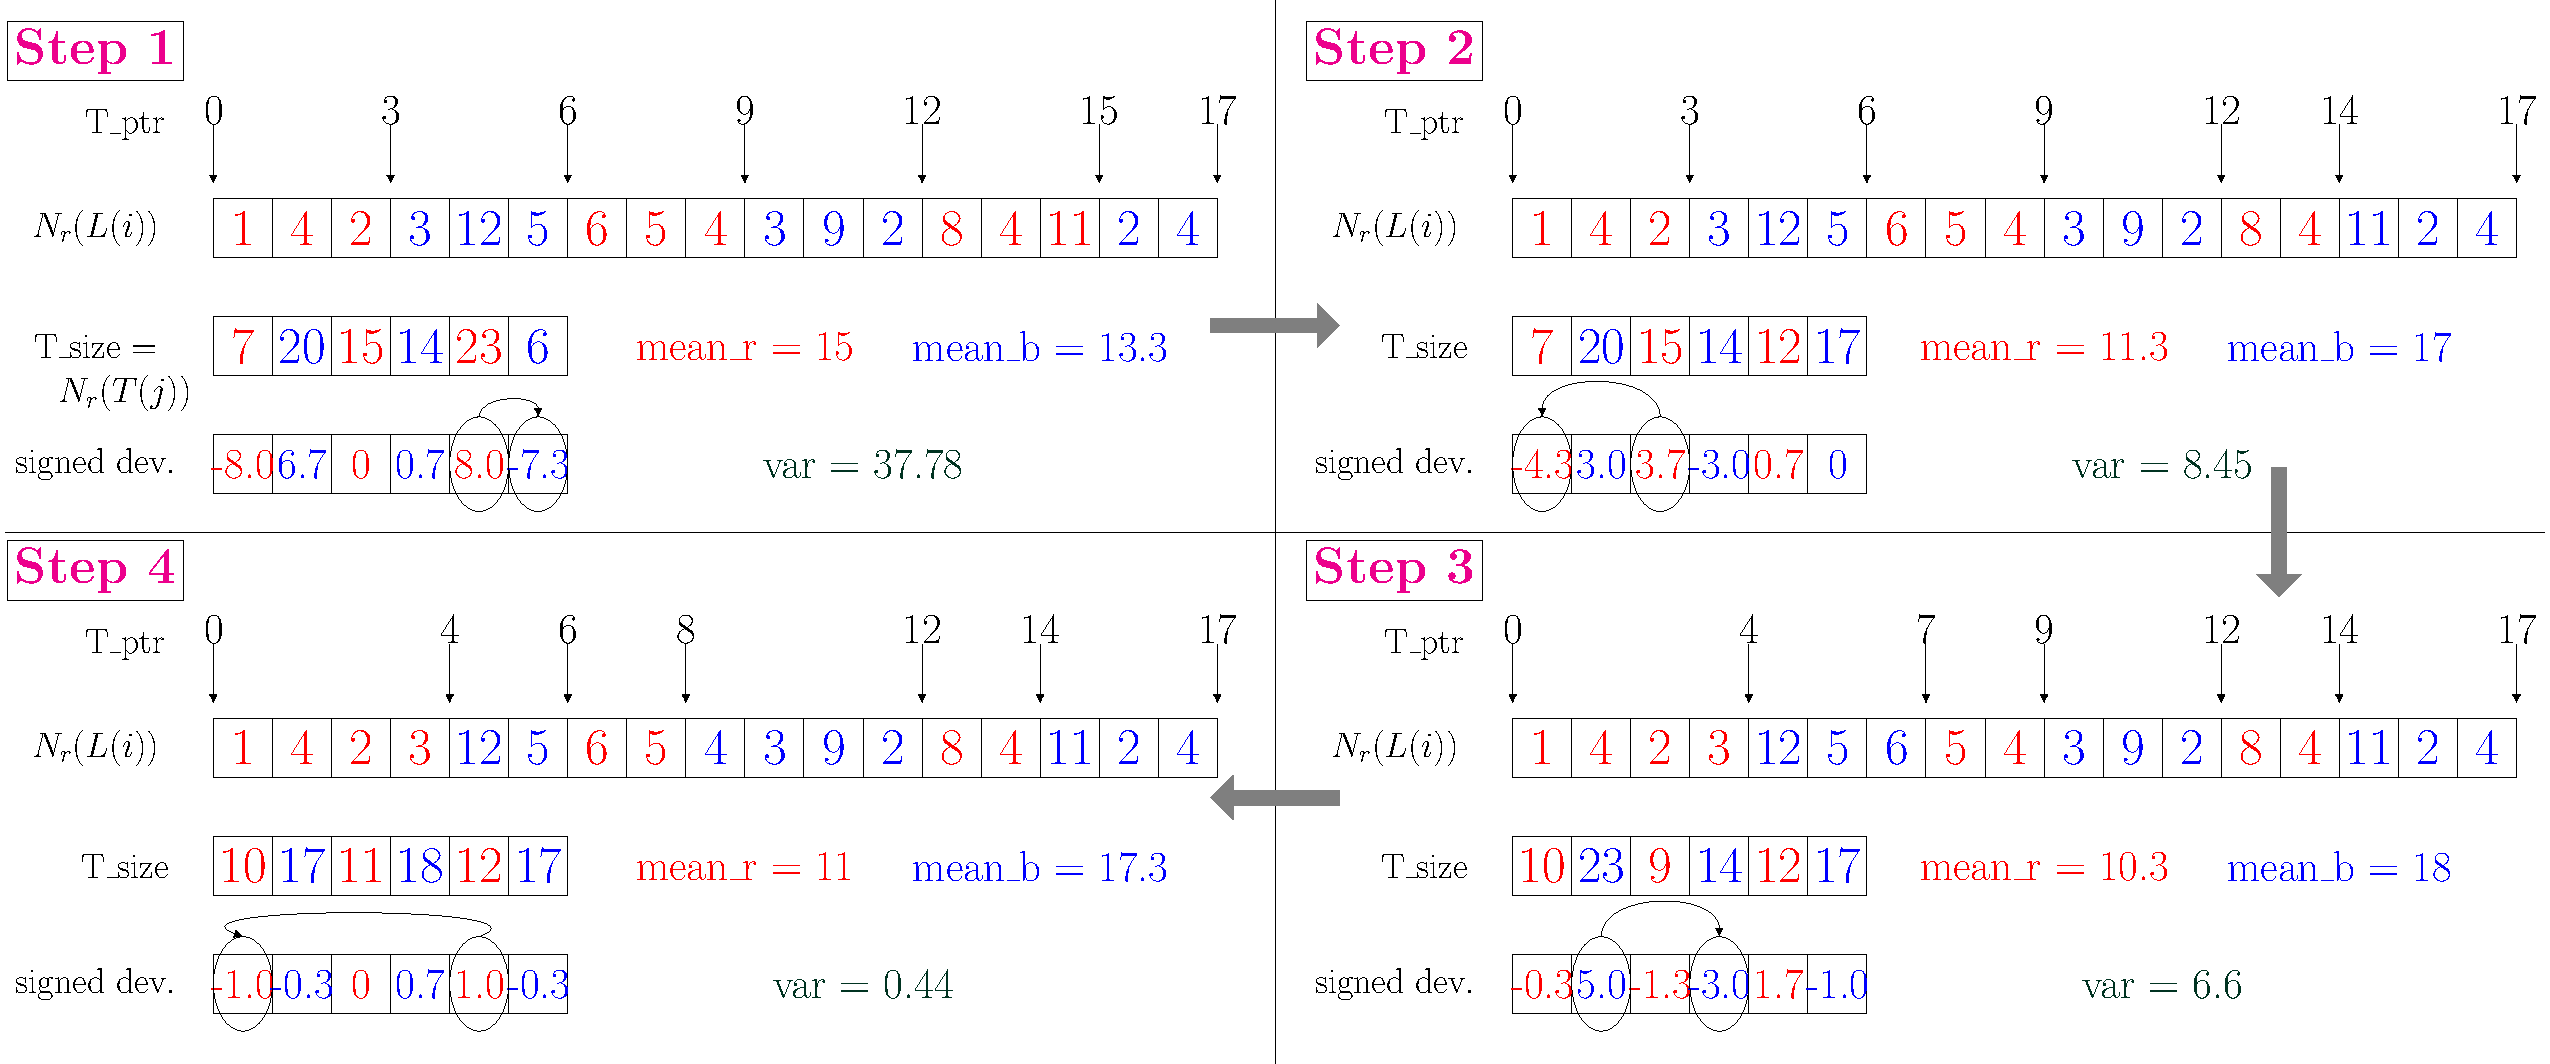
\includegraphics[height=0.22\textheight,width=\textwidth]{pics/load_balancing/lb_alg/lb_all}
   	\caption{All steps of the load balancing scheme applied to an arbitrarily chosen initial distribution of 17 levels into six level groups for \DTWO coloring. Rebalancing steps are performed clockwise starting from top-left. $mean\_r$ and $mean\_b$ denote the current average number of rows per \levelGroup and color. $var$ is the overall  variance}
   	\label{fig:lb_alg}
   \end{figure}
   
   \begin{figure}[t]
	   	\centering
	   	\subfloat[Five threads]{\label{fig:2d_7pt_lb}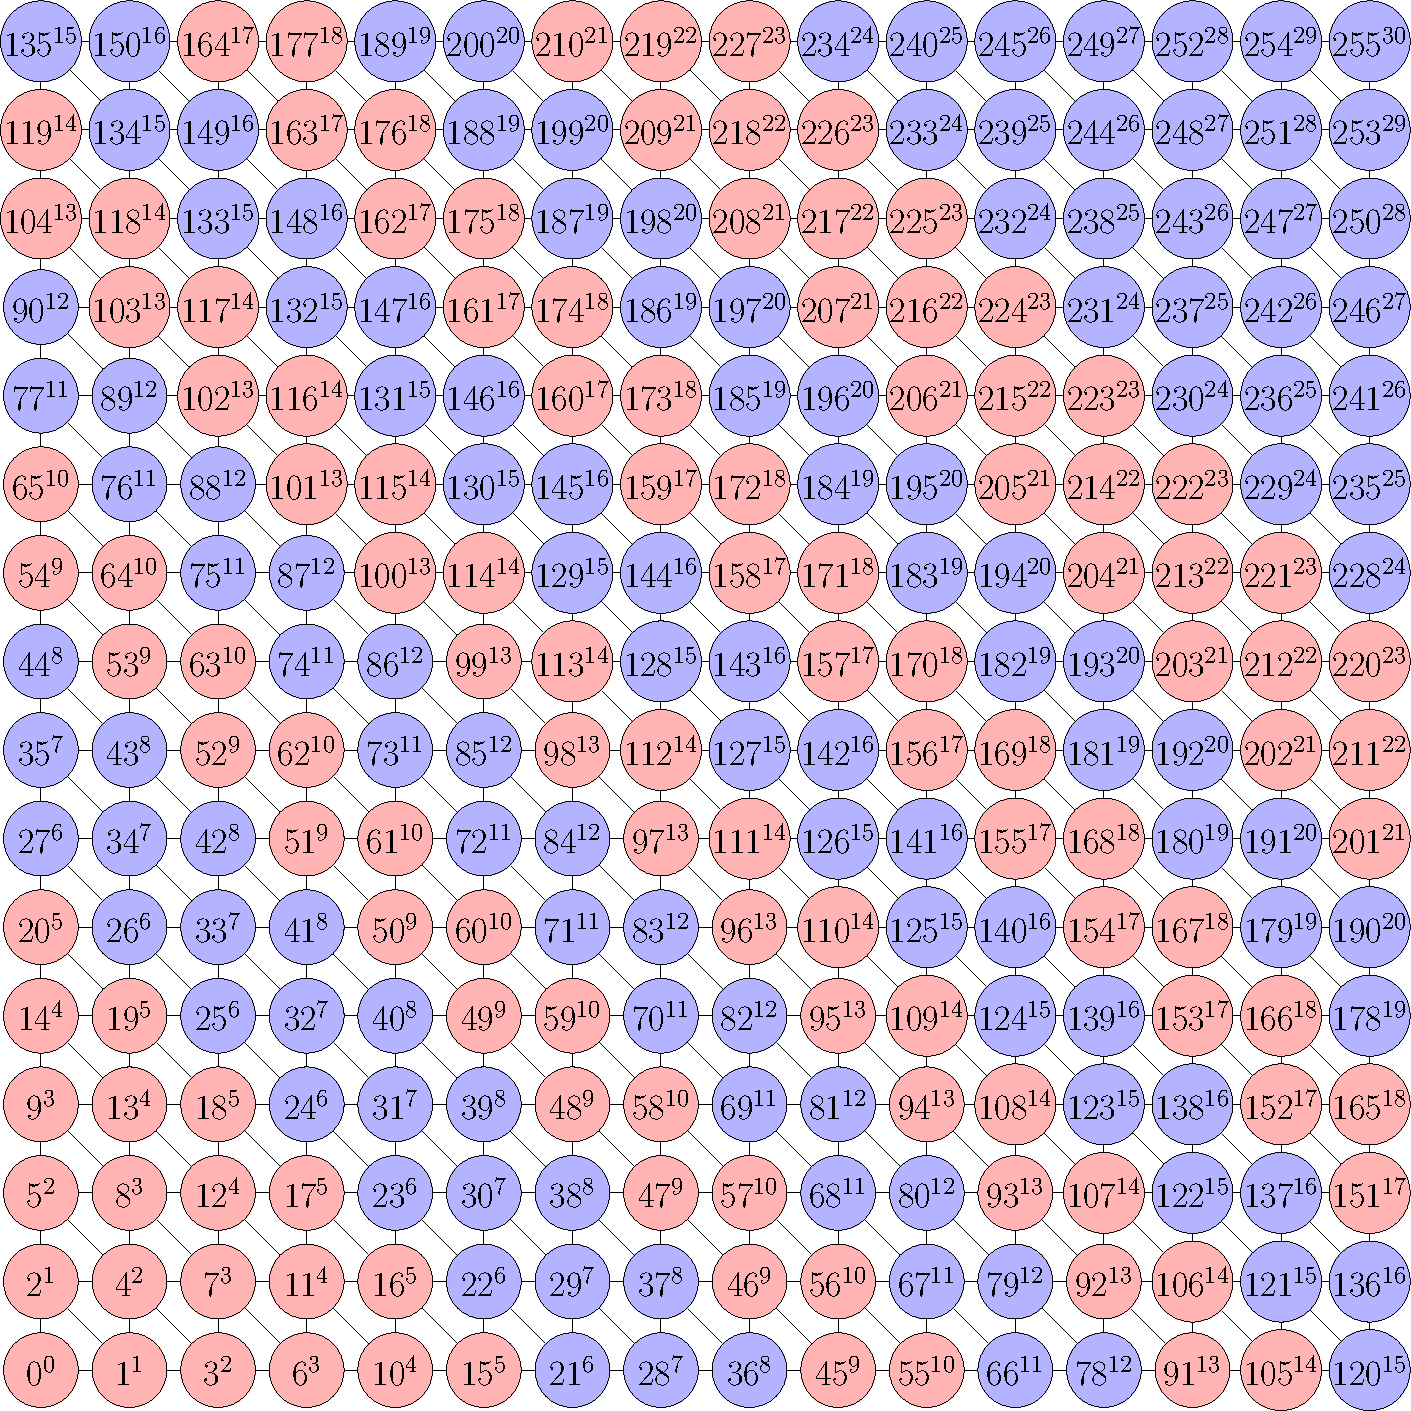
\includegraphics[width=0.48\textwidth, height=0.28\textheight]{pics/load_balancing/2d-7pt/stencil_2d_7pt}}
	   	\hspace{0.2em}
	   	\subfloat[Eight threads]{\label{fig:2d_7pt_lb_8_threads}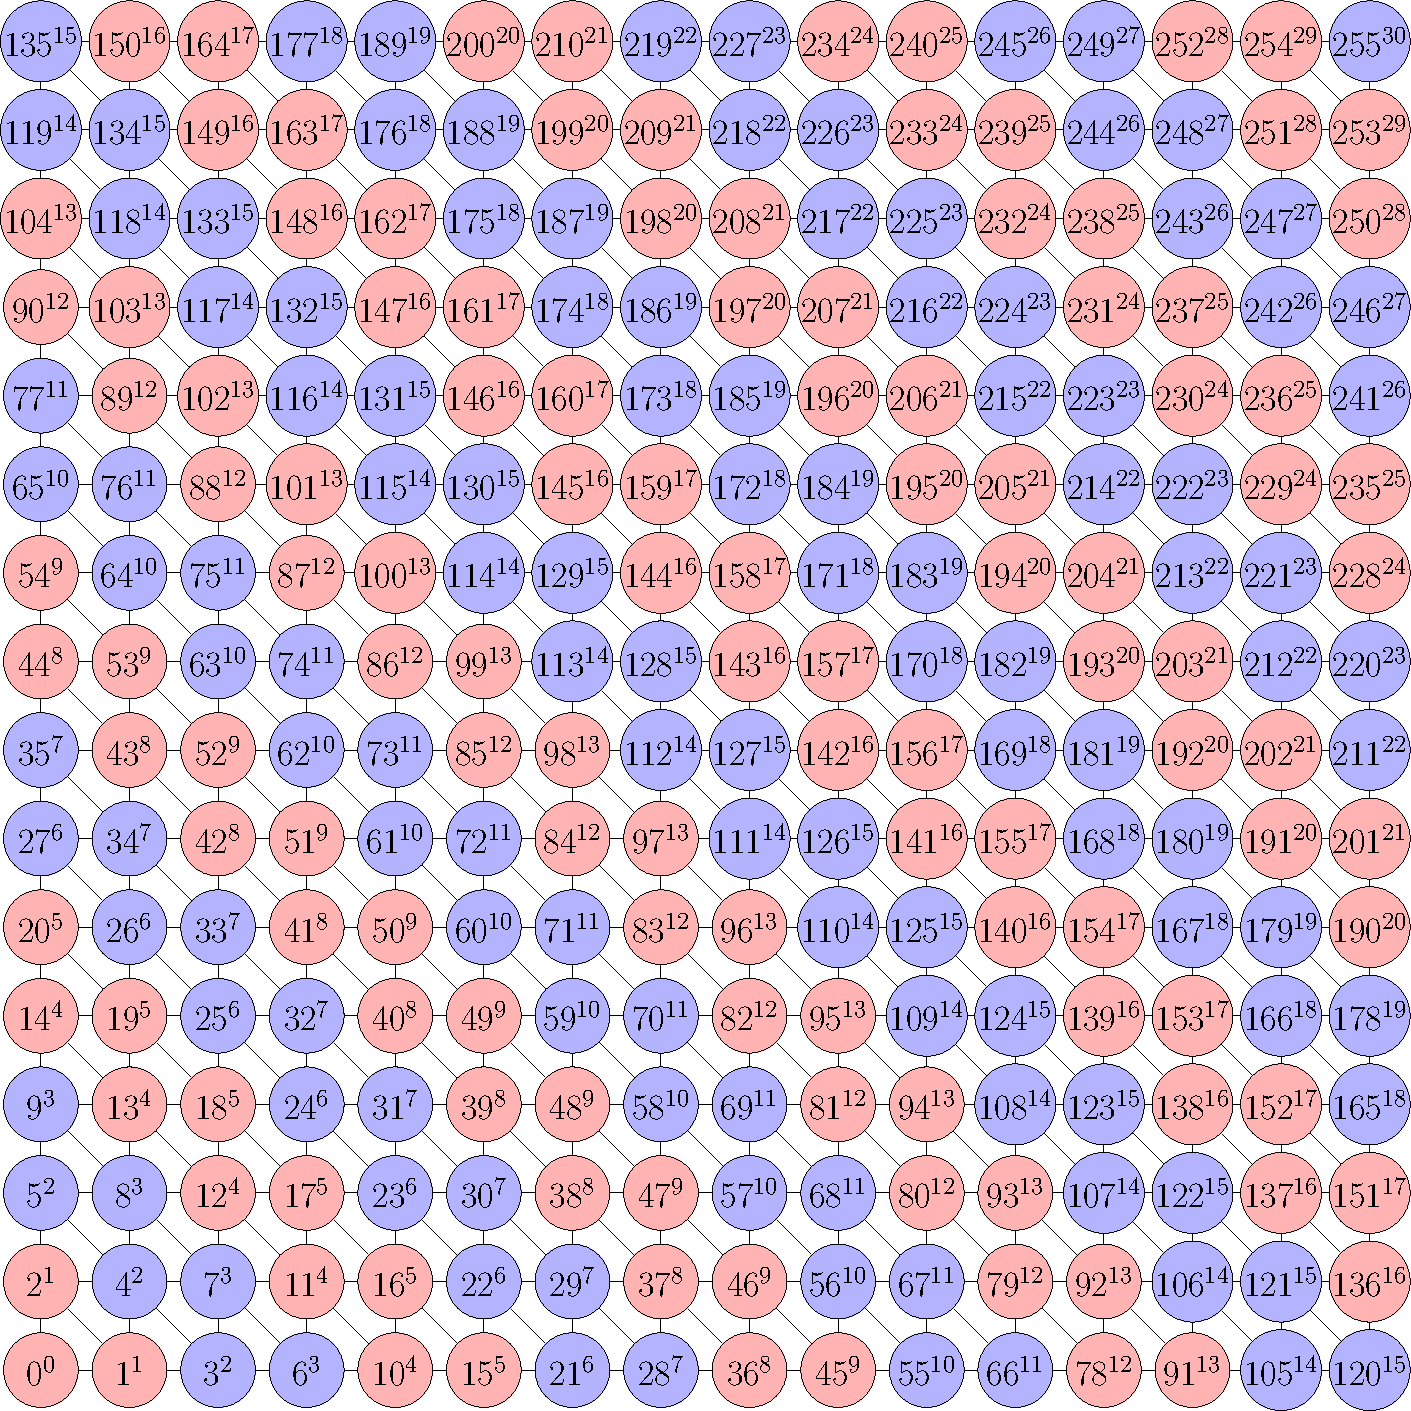
\includegraphics[width=0.48\textwidth, height=0.28\textheight]{pics/load_balancing/2d-7pt/stencil_2d_7pt_8_threads}}
		 \caption{\sref{fig:2d_7pt_lb} after load balancing for five threads and \DTWO dependency for the \stex, domain size $16 \times 16$. 
		 	%Note that \levelGroups at extreme end have more \levels due to fewer \acrshort{nrows} in each \level, while \levelGroups in the middle having bigger \levels maintain two levels to preserve \DTWO constraint. 
		 \sref{fig:2d_7pt_lb_8_threads} after load balancing for eight threads.
		}
	\end{figure}
   

%    \begin{figure}
%      \begin{minipage}[c]{0.63\textwidth}
%      	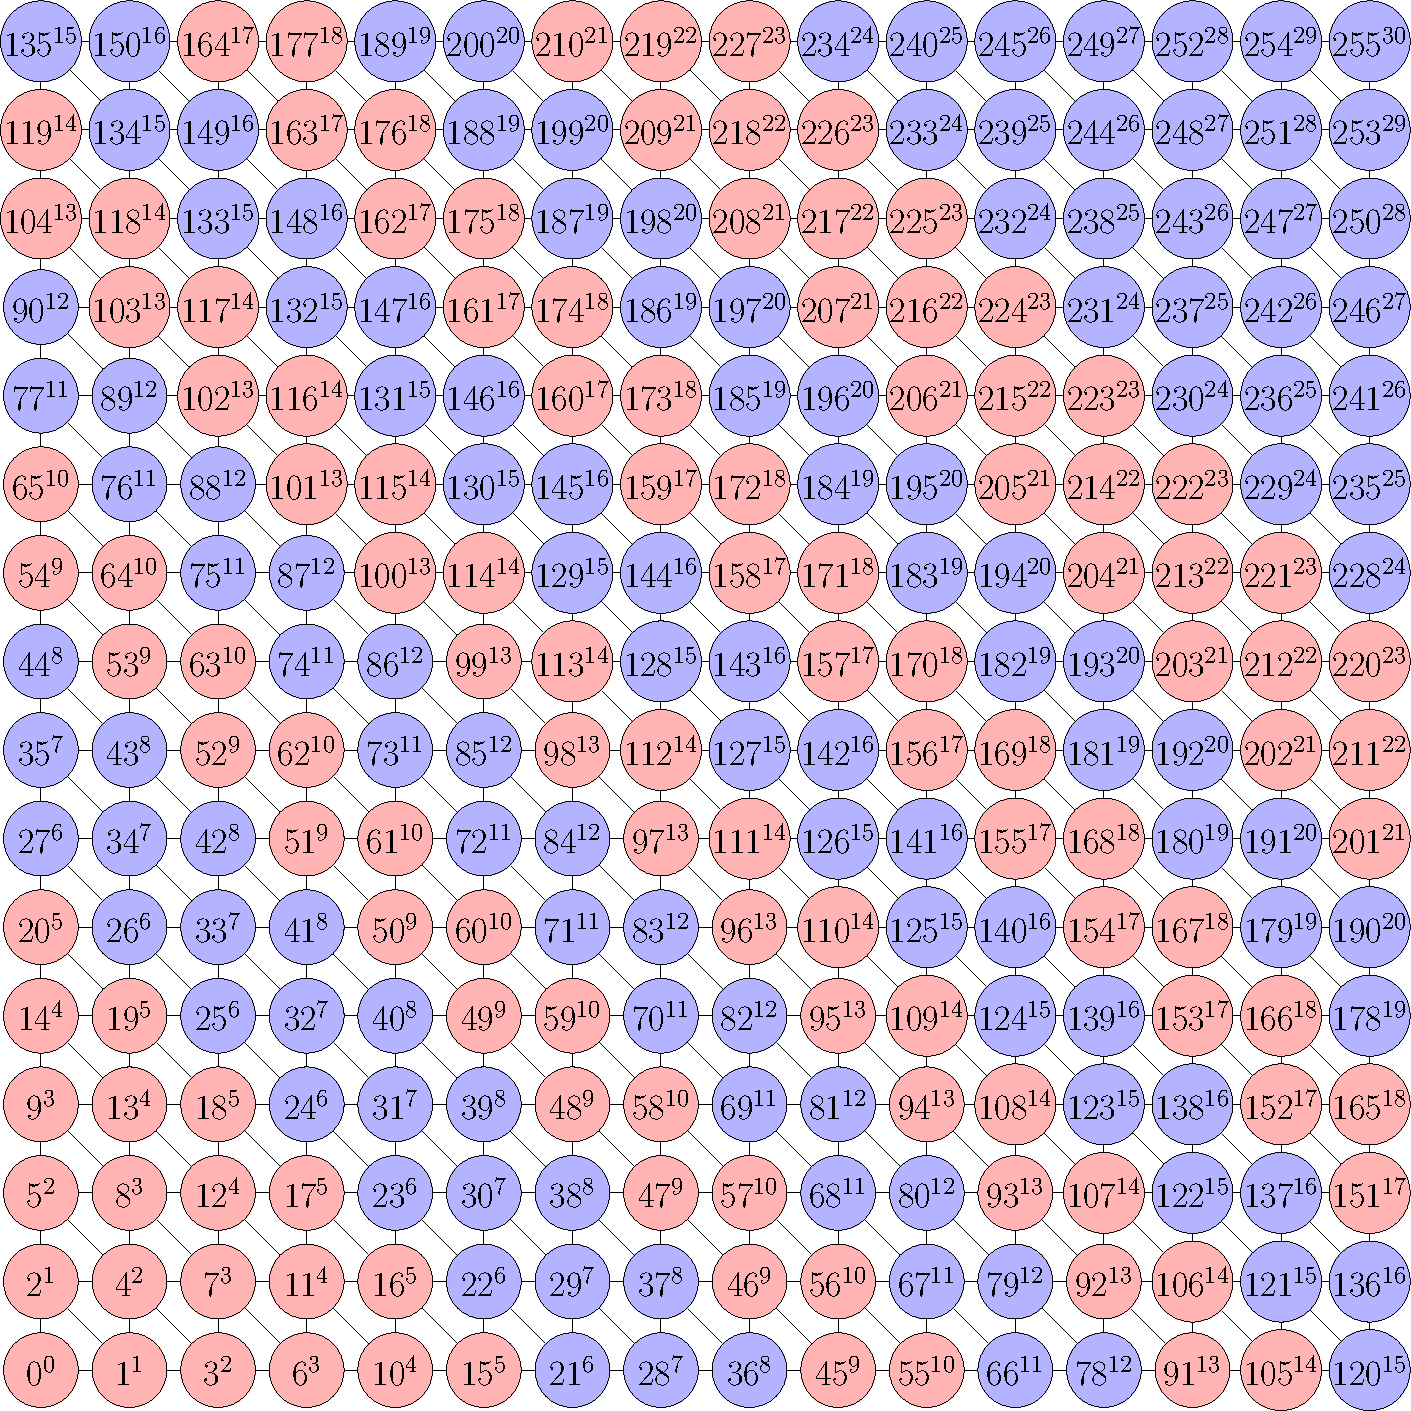
\includegraphics[height=0.26\textheight,width=0.9\textwidth]{pics/load_balancing/2d-7pt/stencil_2d_7pt}
%      \end{minipage}\hfill
%      \begin{minipage}[c]{0.34\textwidth}
%      	\caption{After load balancing for five threads and \DTWO dependency on \stex, domain size $16 \times 16$. Note that \levelGroups at extreme end have more \levels due to fewer \acrshort{nrows} in each \level, while \levelGroups in the middle having bigger \levels maintain two levels to preserve \DTWO constraint.
%      	} \label{fig:2d_7pt_lb}
%      \end{minipage}
%     \end{figure}
%  
%      \begin{figure}
%      	\begin{minipage}[c]{0.63\textwidth}
%      		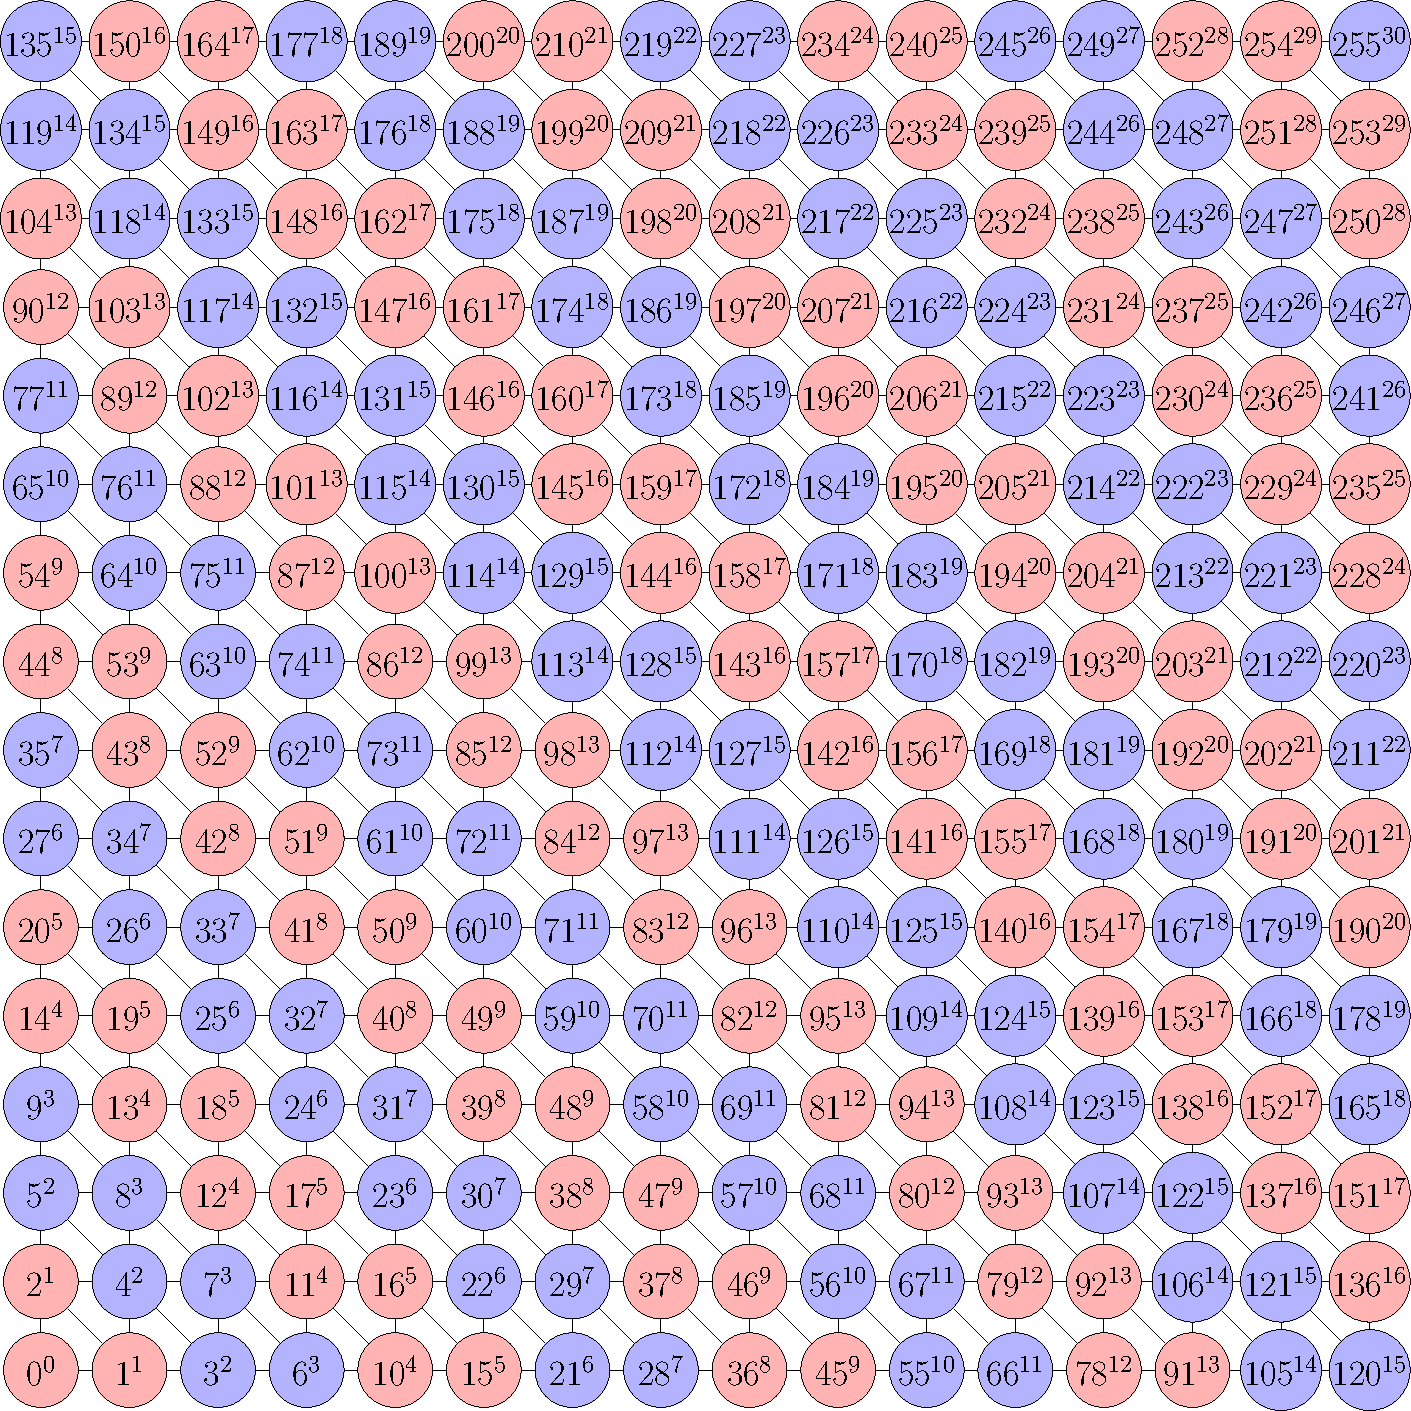
\includegraphics[height=0.26\textheight,width=0.9\textwidth]{pics/load_balancing/2d-7pt/stencil_2d_7pt_8_threads}
%      	\end{minipage}\hfill
%      	\begin{minipage}[c]{0.34\textwidth}
%      		\caption{After load balancing for eight threads and \DTWO dependency on \stex, domain size $16 \times 16$. Note the massive load imbalance between the \levelGroups at extreme ends and in 
%      			the middle. \CAcomm{I am not sure whether we need this, it consumes lot of space and we could explain it with a sentence. TODO: Explain it somewhere}}
%      		 \label{fig:2d_7pt_lb_8_threads}
%      	\end{minipage}
%      \end{figure}  


	\subsection{Recursion}\label{subsec:REC}
As discussed in \Cref{subsec:DK} the maximum degree of parallelism is limited
by the total number of levels (\acrshort{totalLvl}) and may be further reduced 
by level aggregation in the load balancing step. \CAcomm{For example
	requesting the maximum possible eight threads instead of five 
	threads (\Cref{fig:2d_7pt_lb}) for the stencil $16\times16$ example, 
	it results in massive load imbalance as seen in \Cref{fig:2d_7pt_lb_8_threads}. 
Therefore,} to match the high levels of parallelism in modern compute devices we search for 
further parallelism within the \levelGroups.  Compared to methods like \acrshort{MC} 
we didn't require all vertices in a \levelGroup to be \DONE (or \DK in general) 
independent of each other, which is a consequence of our \level based approach 
where we required \DK independency between vertices of different levels but not 
within a level (see \Cref{corollary_dk}). There can exist more parallelism within 
the \levelGroups which we can interpret as \subgraphs.  Thus, we apply the three 
steps of our method recursively on selected \subgraphs to exploit the parallelism 
within them.  
%i.e.  \levelGroups which are recursively refined will be computed by multiple threads whereas unmodified \levelGroups will be assigned to a single thread. 

In the following we first demonstrate in \Cref{subsec:D1_dependency} the basic idea in the context of \DONE dependencies where all dependencies can be resolved within the given \levelGroup by design. However, for $k>1$, vertices in a \levelGroup may have \DK dependencies through vertices in adjacent \levelGroups. We generalize our procedure to \DK dependencies as a second step in \Cref{subsec:Dk_dependency}. Finally, in \Cref{subsec:subgraph_selection} we apply the recursive scheme to our \stex and introduce proper \subgraph selection as well as global load balancing strategies. 

In order to visualize the basic concepts easily and discuss important corner cases of the recursive approach we start with the simple graph shown in \Cref{fig:rec_d1_s1_a}, which is not correlated to our \stex. To distinguish between \levelGroups at different stages \acrshort{s} of our recursive procedure we add a subscript to the levels (\acrshort{L_si}) and \levelGroups (\acrshort{T_si}) indicating the stage of recursion at which they are generated, with $s=0$ being the original distribution before recursion is applied to any \subgraph. 

%also for most of the graphs as we approach the limit of parallelism there is not much room for load balancing, leading to imbalances. Depending on matrix and hardware underneath this might lead to inefficient utilization of resources. \Inorder to avoid this problem we use the concept of recursion and exploit further parallelism if required by the hardware. Idea here is to intelligently select sub-graph(s) of the entire matrix and apply all the three steps recursively on this \subgraph. In the following we will show this concept in the context of \DONE and  later we will extent it to \DK dependencies. In order to explain the basic concepts easily and include all the corner cases we demonstrate the procedure on a simple graph which is shown in \Cref{fig:rec_d1_s1_a}, later we will show the results of applying recursion on \stex. Further we will discuss on the method employed to select proper sub-graph and to have a globally balanced load.
	
	\subsubsection{Distance-$1$ dependency} \label{subsec:D1_dependency}
%\LevelGroups which we constructed till now belong to first stage of recursion ($s=0$). Stage number of recursion is denoted using subscript, \ie for example $L_s(i)$ denotes \level $i$ of stage $s$. Contrary to methods like \acrfull{MC} we didn't require each nodes in a color to be \DONE independent of each other, rather we had a weak constraint as prescribed by \Cref{corollary_dk}. Due to this there can exist more parallelism within a \levelGroup. 

For the \DONE coloring of the graph in \Cref{fig:rec_d1_s1} we find that the third \levelGroup of the initial stage (T$_0$(2)) still contains vertices which are \DONE independent, \eg vertices $3 \not{\xrightarrow{1}} 4$ ($3$  \DONE independent to $4$), $3 \not{\xrightarrow{1}} 5$, $3 \not{\xrightarrow{1}} 6$, and $4 \not{\xrightarrow{1}} 6$, implying each of these pairs can be computed in parallel without any \DONE conflicts. This parallelism has not been exploited in the first stage ($s=0$)  as vertices in $L_0(i)$ (here $i=2$) are chosen such that they are \DONE neighbors of \level $L_0(i-1)$ ignoring any vertex relations in $L_0(i)$. 
%We now apply our method recursively to the levels or \levelGroups to identify further paralleism within them.  	
     \begin{figure}[t]
     	\centering
     	\subfloat[Example graph]{\label{fig:rec_d1_s1_a}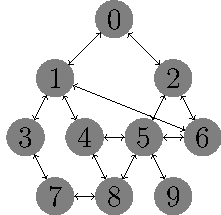
\includegraphics[width=0.26\textwidth, height=0.14\textheight]{pics/recursion/d1/rec_graph_s1/recursion_graph_1}}
     	\hspace{1.5em}
     	\subfloat[Stage 0, levels in graph]{\label{fig:rec_d1_s1_b}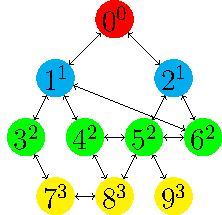
\includegraphics[width=0.26\textwidth, height=0.14\textheight]{pics/recursion/d1/rec_graph_s1/recursion_graph_2}}
     	\hspace{1.5em}
     	\subfloat[\DONE coloring]{\label{fig:rec_d1_s1_c}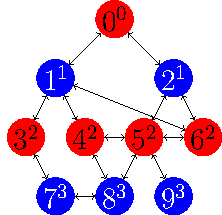
\includegraphics[width=0.26\textwidth, height=0.14\textheight]{pics/recursion/d1/rec_graph_s1/recursion_graph_3}}
        \caption{Shows potential for more parallelism. $T_0(1),T_0(2),$ and $T_0(3)$ have more parallelism. Note that the graph shown here is not related to the previous \stex.}
     	\label{fig:rec_d1_s1}
     \end{figure}

Recursion starts with the selection of a \subgraph of the matrix, which is discussed in more detail later (see \Cref{subsec:subgraph_selection}). Here we choose a \subgraph induced by $T_0(2)$. The  \subgraph can be isolated from the rest of the graph since the \DONE coloring step in stage 0 has already made \levelGroups independent of each other. Now we just need to repeat the three steps explained previously (\Cref{subsec:LEVEL_CONST}--\Cref{subsec:LB}) on this \subgraph.
%to exploit parallelism within this \subgraph.
   
     \begin{figure}[t]
     	\centering
     	\subfloat[]{\label{fig:rec_d1_s2_a}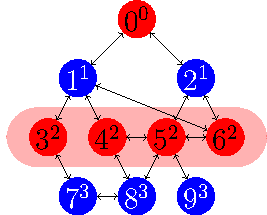
\includegraphics[width=0.28\textwidth, height=0.14\textheight]{pics/recursion/d1/rec_graph_s2/recursion_graph_stage2_1}}
     	\hspace{2.25em}
     	\subfloat[]{\label{fig:rec_d1_s2_b}
\includegraphics[width=0.07\textwidth, height=0.14\textheight]{pics/recursion/d1/rec_graph_s2/recursion_graph_stage2_2}}
     	\hspace{1.75em}
     	\subfloat[]{\label{fig:rec_d1_s2_c}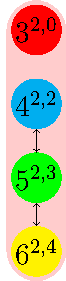
\includegraphics[width=0.065\textwidth, height=0.14\textheight]{pics/recursion/d1/rec_graph_s2/recursion_graph_stage2_3}}
     	\hspace{1.75em}
     	\subfloat[]{\label{fig:rec_d1_s2_d}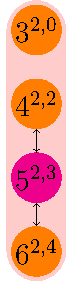
\includegraphics[width=0.065\textwidth, height=0.14\textheight]{pics/recursion/d1/rec_graph_s2/recursion_graph_stage2_4}}
	     \hspace{1.75em}
	     \subfloat[]{\label{fig:rec_d1_s2_e}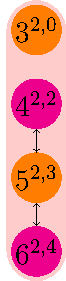
\includegraphics[width=0.065\textwidth, height=0.14\textheight]{pics/recursion/d1/rec_graph_s2/recursion_graph_stage2_5}}
     	\caption{Applying recursion to the \subgraph induced by $T_0(2)$. \Cref{fig:rec_d1_s2_b} shows the isolated \subgraph, \Cref{fig:rec_d1_s2_c} presents the level construction step on the \subgraph. Two potential \DONE colorings of this  \subgraph are shown in \Cref{fig:rec_d1_s2_d,fig:rec_d1_s2_e}.}
     	
     	\label{fig:rec_d1_s2}
     \end{figure}
     
     \Cref{fig:rec_d1_s2} shows an illustration of applying the first recursive step ($s=1$) on $T_0(2)$, where we extend the definition of the vertex numbering in \Cref{eq:node_notation} to the following:
	 \begin{equation}
	    v^{i,j,k...} \implies v \in \set{L_0(i) \cap L_1(j) \cap L_2(k) \cap \cdots}.
	 \end{equation}
	 
     In this case at the end of the recursion (\cf \Cref{fig:rec_d1_s2_d,fig:rec_d1_s2_e}) on $T_0(2)$ we obtain parallelism for two more threads. Note that the \subgraphs might have islands (group of vertices that are not connected to the rest of the graph), \eg vertex 3 and vertices 4,5,6 form two islands in \Cref{fig:rec_d1_s2_b}. Since an island is totally disconnected from the rest of the (sub)graph it can be executed in parallel to the rest of the (sub)graph. To take advantage of this the starting node in the next island is assigned with an increment of two levels, as seen in \Cref{fig:rec_d1_s2_c}. Therefore multiple valid \DONE configurations (\cf \Cref{fig:rec_d1_s2_d,fig:rec_d1_s2_e}) exist and the selection of the optimal one will be done in the final load balancing step as described in \Cref{subsec:LB}.    
     
     With this recursive process we were able to find independent \levelGroups ($T_{s+1}$) within a \levelGroup of the previous stage ($T_s$) and therefore the thread which works on $T_s$ has to spawn threads to parallelize within $T_{s+1}$.
     
	\subsubsection{Distance-$k$ dependencies with $k>1$}  \label{subsec:Dk_dependency}
In general, however, it is not sufficient in the recursion step to consider only the \subgraphs induced by \levelGroups as can be seen in \Cref{fig:rec_d2_wrong_a} for \DTWO coloring. Applying  the three steps (see \Cref{fig:rec_d2_wrong_b,fig:rec_d2_wrong_c,fig:rec_d2_wrong_d})  to  the \subgraph induced by $T_0(1)$ does not guarantee \DTWO independence between the new \levelGroups $T_1(0)$ and $T_1(2)$. It is obvious that for general \DK colorings two vertices $a,b$ within a \levelGroup might be connected by a shared vertex $c$ outside the \levelGroup.  \CAcomm{Thus, our three step procedure must be applied to a \subgraph which contains the actual \levelGroup ($T_s(j)$) as well as its all distance-$p$ neighbors, where $p=1,2,\ldots,(k-1)$.}
%as they
%For \DK the same procedure as \DONE applies, except with a slight difference in selecting the \subgraph. In \DONE we considered \subgraphs induced by \levelGroups, but for \DK coloring this is not sufficient. As seen in \Cref{fig:rec_d2_wrong_a} for \DTWO coloring the selection of $T_0(1)$ as \subgraph and applying the three steps (see \Cref{fig:rec_d2_wrong_b}, \Cref{fig:rec_d2_wrong_c} and \Cref{fig:rec_d2_wrong_d}) did not guarantee \DTWO independency within \levelGroup $T_1$ of the \subgraph, for \eg $T_1(0)$ and $T_1(2)$ are not \DTWO independent (\cf \Cref{fig:rec_d2_wrong_d}). This is due to the fact that for $k>1$ dependencies two vertices $a,b$ within a \subgraph might be connected to a common vertex ($c$) outside the \subgraph leading to a \DK dependency between $a$ and $b$. In \Cref{fig:rec_d2_wrong} we see 	$3 \xrightarrow{1} 1 \text{ \& } 6 \xrightarrow{1} 1 	\implies 3 \xrightarrow{2} 6$, but since vertex $1$ was not in the \subgraph considered we missed this dependency. 
     \begin{figure}[t]
     	\centering
     	\subfloat[]{\label{fig:rec_d2_wrong_a}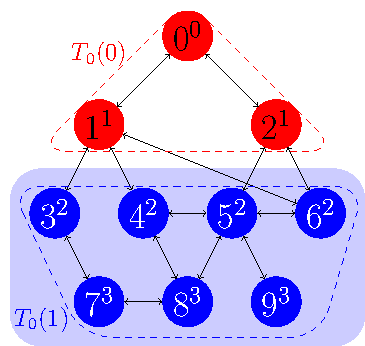
\includegraphics[width=0.23\textwidth, height=0.13\textheight]{pics/recursion/d2/wrong/recursion_graph_wrong_1}}
     	\hspace{0.6em}
     	\subfloat[]{\label{fig:rec_d2_wrong_b}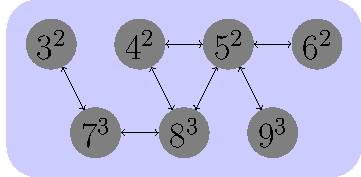
\includegraphics[width=0.23\textwidth, height=0.07\textheight]{pics/recursion/d2/wrong/recursion_graph_wrong_2}}
     	\hspace{0.6em}
     	\subfloat[]{\label{fig:rec_d2_wrong_c}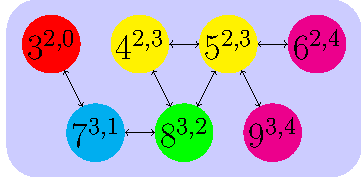
\includegraphics[width=0.23\textwidth, height=0.07\textheight]{pics/recursion/d2/wrong/recursion_graph_wrong_3}}
     	\hspace{0.6em}
     	\subfloat[]{\label{fig:rec_d2_wrong_d}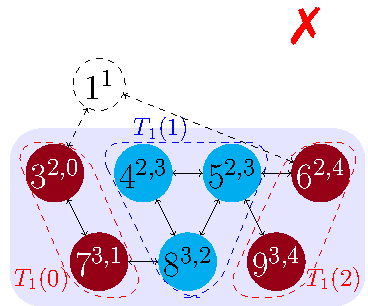
\includegraphics[width=0.23\textwidth, height=0.13\textheight]{pics/recursion/d2/wrong/recursion_graph_wrong_4}}
     	\caption{Two \levelGroups generated by a \DTWO coloring (\Cref{fig:rec_d2_wrong_a}). \Cref{fig:rec_d2_wrong_b} shows the \subgraph induced by \levelGroup $T_0(1)$. Level construction on the selected \subgraph is shown in \Cref{fig:rec_d2_wrong_c}. Forming \DTWO independent \levelGroups on these levels does not guarantee a \DTWO independence between the newly generated \levelGroups of the same sweep (color) as seen in \Cref{fig:rec_d2_wrong_d}.}
     	\label{fig:rec_d2_wrong}
     \end{figure}

%\begin{equation*}
%	   N^{k-1}(T_s(j)) = \set{u : u \xrightarrow{k-1} v \text{  } \forall v \in T_s(j) \text { and } u \notin T_s(j)}.
%\end{equation*}

This ensures that there is no vertex outside the \subgraph which can mediate a \DK dependency between vertices in the embedded \levelGroup ($T_s(j)$). We can now construct the new levels on this \subgraph considering the neighborhood but only store the vertices in the new \levels $L_{s+1}(:)$ which are in the embedded \levelGroup ($T_s(j)$). Next we apply \DK coloring by aggregation of the new levels leading to a set of \levelGroups $T_{s+1}(:)$ within $T_s(j)$. \Cref{fig:rec_d2_correct} uses this approach to resolve the conflict demonstrated in \Cref{fig:rec_d2_wrong_d}. \Cref{fig:rec_d2_correct_b} presents the \subgraph containing the selected \levelGroup $T_0(1)$ and its \DONE neighborhood. %For \DTWO this would mean we have to include $1^{st}$ interface level, the new selection is illustrated in \Cref{fig:rec_d2_correct} (note the region shaded in blue). If we then do all the three steps with the newly created \subgraph, the final result will preserve \DTWO coloring (see \Cref{fig:rec_d2_correct_c}). In the example it can be observed vertices $3$ and $6$ which previously had same color now get assigned to different colors (see \Cref{fig:rec_d2_correct_d}). Note that the interface levels have to be considered only in the first step namely level construction in the rest of the steps we just need to consider target \subgraphs induced by the \levelGroups \ie in \Cref{fig:rec_d2_correct} the \subgraph induced by $T_0(1)$.   
\begin{figure}[t]
     	\centering
     	\subfloat[]{\label{fig:rec_d2_correct_a}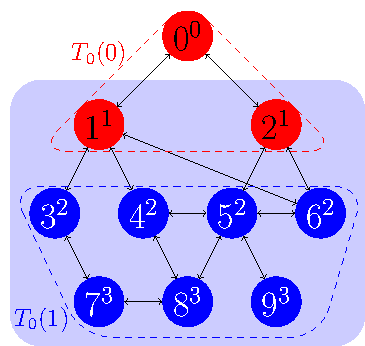
\includegraphics[width=0.22\textwidth, height=0.13\textheight]{pics/recursion/d2/correct/recursion_graph_correct_1}}
     	\hspace{0.6em}
     	\subfloat[]{\label{fig:rec_d2_correct_b}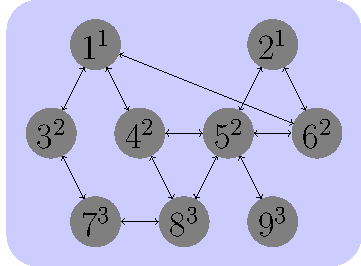
\includegraphics[width=0.22\textwidth, height=0.105\textheight]{pics/recursion/d2/correct/recursion_graph_correct_2}}
     	\hspace{0.6em}
     	\subfloat[]{\label{fig:rec_d2_correct_c}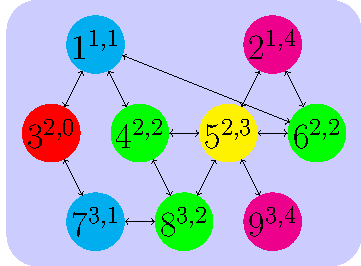
\includegraphics[width=0.22\textwidth, height=0.105\textheight]{pics/recursion/d2/correct/recursion_graph_correct_3}}
     	\hspace{0.6em}
     	\subfloat[]{\label{fig:rec_d2_correct_d}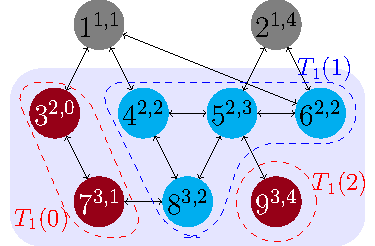
\includegraphics[width=0.22\textwidth, height=0.105\textheight]{pics/recursion/d2/correct/recursion_graph_correct_4}}
     	\hspace{0.6em}
     	\caption{Correct procedure for \DTWO coloring of \levelGroup $T_0(1)$. The \subgraph as shown in \Cref{fig:rec_d2_correct_b} contains \levelGroup $T_0(1)$ and its \DONE neighborhood. A level construction step is applied to this \subgraph in \Cref{fig:rec_d2_correct_c}. Distance-2 coloring by level aggregation leading to \levelGroups of stage 1 is shown in \Cref{fig:rec_d2_correct_d}; we get three \levelGroups at the end of the recursion on $T_0(1)$.}
     	\label{fig:rec_d2_correct}
     \end{figure}
Level construction is performed on the \subgraph (\Cref{fig:rec_d2_correct_c}) but the new levels only contain vertices of  $T_0(1)$, \ie $L_1(1) = \{7^{3,1}\}$. Finally, \DTWO coloring by aggregation of two adjacent levels is performed, leading to three \levelGroups of the second stage $s=1$ (\Cref{fig:rec_d2_correct_d}), \ie $T_1(0)=\{L_1(0) \cup L_1(1)\}$.  Now vertices $3$ and $6$ are mapped to \levelGroups of different colors. Note, that the permutation step on the newly generated levels is not shown but is performed as well to maintain data locality. 
    
%We finally apply the recursive step to the coloring shown in \Cref{fig:2d_7pt_lb} where parallelism is restricted to five threads at a time.  To increase parallelism to eight threads we do apply our recursive approach 
%Requesting parallelism for eight threads for our \stex with \DTWO independency instead of five threads (see result of our procedure applying one recursive step to \levelGroups $T_0(4),T_0(5),T_0(6)$ and $T_0(7)$ is seen in \Cref{fig:rec_2d-7pt_graph} (left). 
%In \Cref{fig:rec_2d-7pt_graph} we demonstrate the impact of one recursive step applied to our \stex with \DTWO 
       \begin{figure}[t]
       	\begin{minipage}[c]{0.6\textwidth}
       		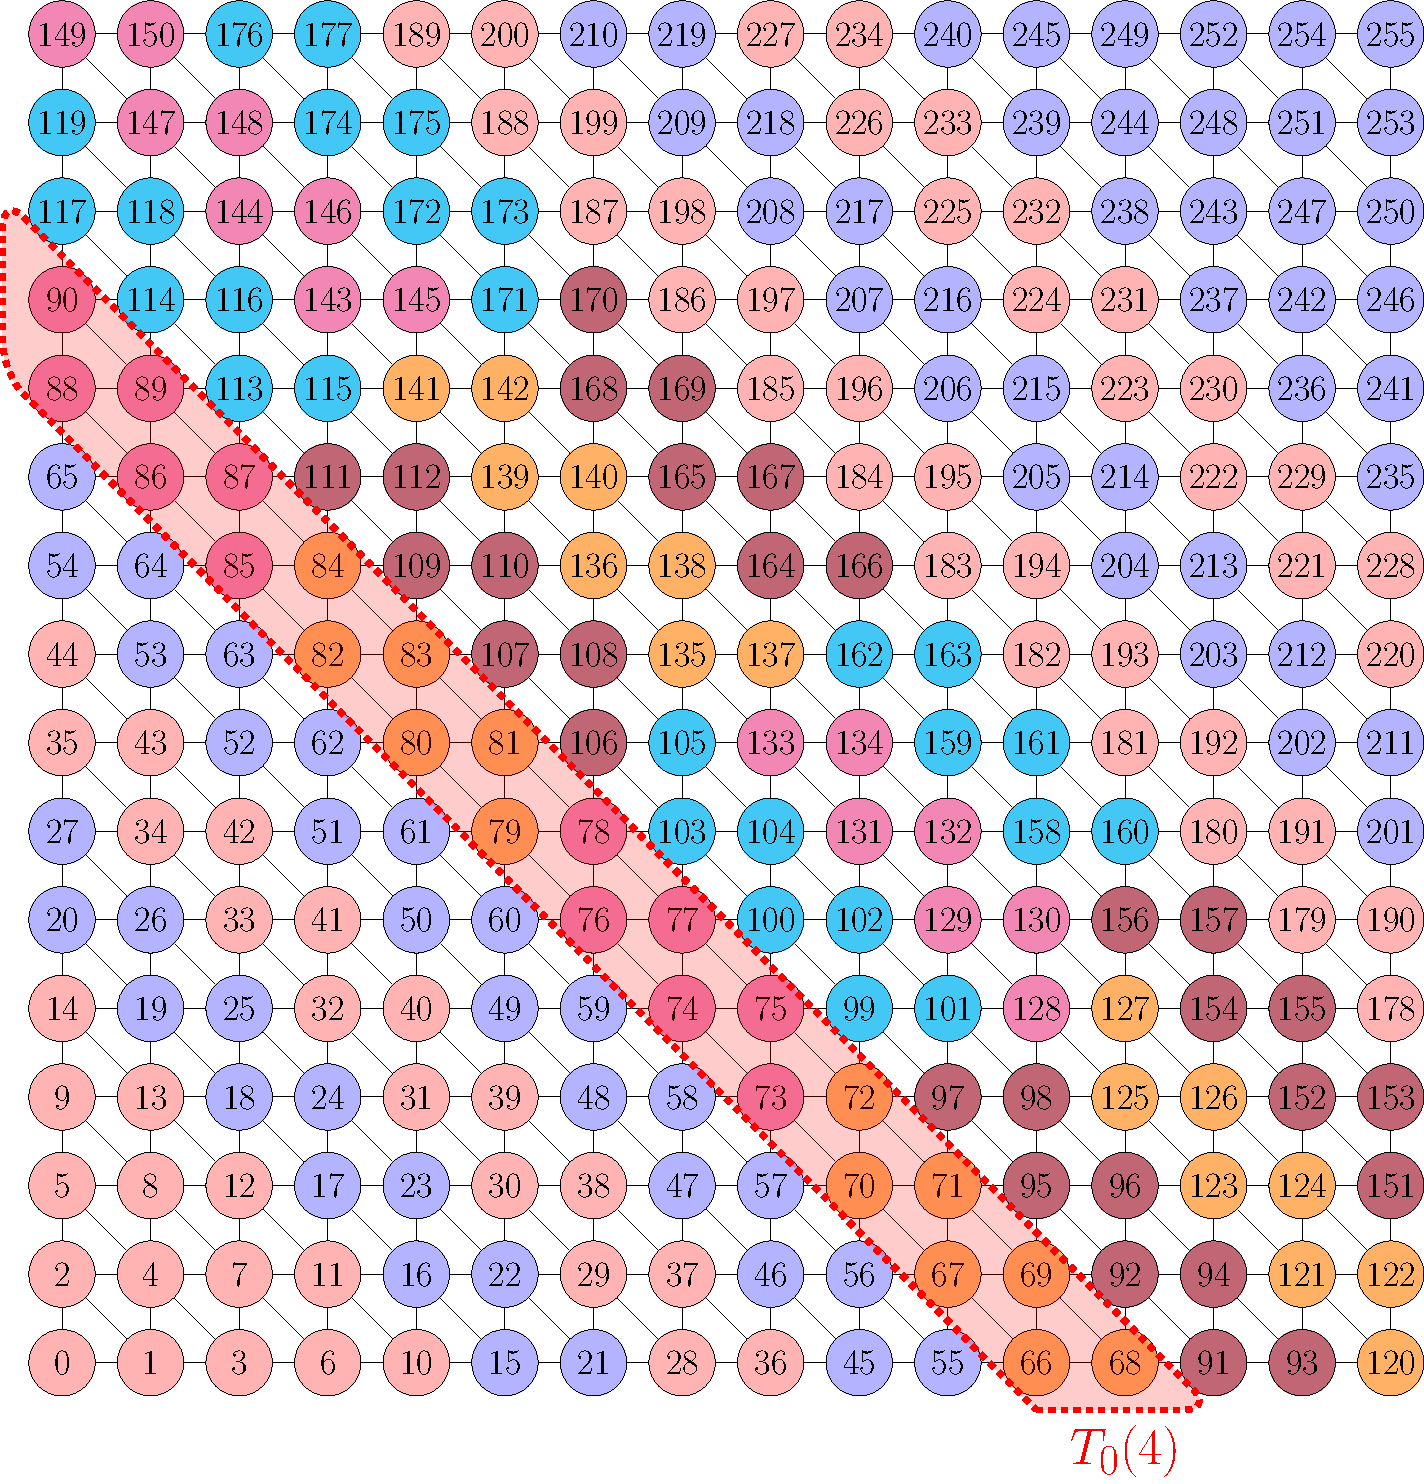
\includegraphics[height=0.3\textheight,width=0.89\textwidth]{pics/recursion/2d-7pt_example/2d-7pt/stencil_2d_7pt}
       	\end{minipage}\hfill
       	\begin{minipage}[c]{0.4\textwidth}
       	%	{\tt for parallel all \textcolor{red}{red}\\
       	%		\hspace*{1em} for parallel all \textcolor{amber}{orange}\\
       	%		\hspace*{1em} for parallel all \textcolor{magenta}{pink}\\
       	%	}
       	%	{\tt for parallel all \textcolor{blue}{blue}\\
       	%		\hspace*{1em} for parallel all \textcolor{carmine}{brown}\\
       	%		\hspace*{1em} for parallel all \textcolor{cyan}{cyan}\\
       	%	}
	       	\begin{tabular}{l|l}
	    %   		\toprule
	       		{Initial Stage} & {Recursion}\\
	       		{($s=0$)} & {($s=1$)}\\
	       		\midrule
	       	   \multirow{2}{*}{\textcolor{red}{red}} & {\textcolor{amber}{orange}}\\
	       	   \rule{0pt}{3ex}
	       	   %\cmidrule(lr){2-2}
	       		& {\textcolor{magenta}{pink}}\\
				\rule{0pt}{4ex} 
	       	   \multirow{2}{*}{\textcolor{blue}{blue}} & {\textcolor{carmine}{brown}}\\
	       	   %\cmidrule(lr){2-2}
	       	   \rule{0pt}{3ex}
	       	   & {\textcolor{cyan}{cyan}}\\
	       	   %\bottomrule
	       	\end{tabular}
	       	\begin{tikzpicture}[overlay]
		       	\draw[-, dashed, red, line width=1.5] (-1.8,0.22) -- (-0.1,0.22);
		       	\draw[-, dashed, red, line width=1.5] (-3.9,-0.4) -- (-0.1,-0.4);
		      	\draw[-, dashed, red, line width=1.5] (-1.8,-1.05) -- (-0.1,-1.05);
		       	\draw[-, dashed, red, line width=1.5] (-3.9,-1.6) -- (-0.1,-1.6);
		       	\draw[->] (0.2,0.7) -- (0.2,-1.5);
		       	\node[rotate=-90] at (0.45,-0.4) {execution time};
	       	\end{tikzpicture}
       		\caption{Graph coloring of the \stex for eight threads. Recursion is applied on \levelGroups $T_0(4-7)$ with two threads assigned to each. The parallel execution order is shown on the right.  Horizontal red dotted lines indicate synchronization and its extent. Vertical lines distinguish between \levelGroups of different stages (here $T_0$ and $T_1$) which can run in parallel. 
		%{\GW do i need to synchronize all threads working on orange color? or only those within the original \levelGroup, e.g. $T_0(4)$ ?} } {\CA only those within original \levelGroup $T_0(4)$, that is the reason why I used the term nested parallelism
		}
       		\label{fig:rec_2d-7pt_graph}
       	\end{minipage}
       \end{figure}
     
%Here we see recursion is applied to \levelGroups $T_0(4),T_0(5),T_0(6)$ and $T_0(7)$. In this case each of the \levelGroups where recursion is applied spawns parallelism for two threads. The selection of \levelGroups to refine and number of threads needed from each recursion are determined using a global load balancing technique as will be explained in \Cref{subsec:subgraph_selection}.
%\Cref{fig:rec_2d-7pt_graph} (right) shows the execution order of different \levelGroups. Note the usage of nested parallelism, \ie for example thread responsible for $T_0(4)$ spawns two child threads to execute $T_1(0) \subset T_0(4)$ and $T_1(2) \subset T_0(4)$ in one parallel sweep, and $T_1(1) \subset T_0(4)$ and $T_1(3) \subset T_0(4)$ in next parallel sweep. At the end of each sweep there is synchronization between threads assigned to \levelGroup of similar color as represented by a horizontal bar in \Cref{fig:rec_2d-7pt_graph} (right). Since each of the leaves needs to synchronize only with it's siblings (leaves of same parent)  we use a simple point to point synchronization scheme. 
          
\subsubsection{Level group construction and global load balancing} \label{subsec:subgraph_selection}

The recursive refinement of \levelGroups allows us to tackle load imbalance problems and limited degree of parallelism as we are no longer restricted by the one thread per \levelGroup constraint.  Instead we have the opportunity to form \levelGroups and assign appropriate thread counts to them such that the load per thread approaches the optimal value, \ie total workload divided by the number of threads available. For simplicity we enforce an equal number of threads to adjacent \levelGroups having different color, \ie $T_s(i)$ and $T_s(i+1)$ with $i=0,2,4,...$. We then apply recursion to the \levelGroups with more than one thread assigned. Starting with the original graph as the base \levelGroup ($T_{-1}(0)$) to which all available threads $\acrshort{nthreads}(T_{-1}(0))=\acrshort{nthreads}$ and all vertices $\acrshort{nrows}(T_{-1}(0))=\acrshort{nrows}^{total}$ are assigned, we perform the following steps to form \levelGroups $T_s(:)$ at stage $s \ge 0$  to which we assign $\acrshort{nthreads}(T_{s}(:))$ threads. To show the procedure we use the $16 \times 16$ \stex and construct a coloring scheme for eight threads (see \Cref{fig:rec_2d-7pt_graph}).

\begin{enumerate}
	\item  Assign weights to all levels at stage ($s$) of the recursion. Assuming that $L_s(i) \subset T_{s-1}(j)$, its weight is defined by
	
	\begin{align*}
		w(L_s(i)) &= \frac{\acrshort{nrows}(L_s(i))}{\frac{\acrshort{nrows}(T_{s-1}(j))}{\acrshort{nthreads}(T_{s-1}(j))}} = \frac{\acrshort{nrows}(L_s(i))}{\acrshort{nrows}(T_{s-1}(j))}  \acrshort{nthreads}(T_{s-1}(j)).\\
%		\acrshort{nthreads} &: \text{total number of threads to be used for computing $T_{s-1}(j)$}\\
%		\nrowsMath^{total} &\acrshort{nrows}= n_r(T_{s-1}(j)) %\text{, i.e. number of vertices in graph}
	\end{align*}
	%In the initial stage ($s=0$) the base \levelGroup ($T_{-1}(0)$) is the full matrix/graph and $\acrshort{nthreads}$ is the total number of threads available. 
	%This weight describes the fraction of the optimal load per thread ($\frac{n_r(T_{s-1}(j))}{\acrshort{nthreads}(T_{s-1}(j))}$) in the specific level ($L_s(i)$) for a given \levelGroup ($T_{s-1}(j)$) which has to be split up, i.e.  $\acrshort{nthreads}(T_{s-1}(j)) > 1$
	%{\CA May be rewrite sentence before as:}
	
	 For a given \levelGroup ($T_{s-1}(j)$) that has to be split up ( $\acrshort{nthreads}(T_{s-1}(j)) > 1$), the weight describes the fraction of the optimal load per thread  ($\frac{\acrshort{nrows}(T_{s-1}(j))}{\acrshort{nthreads}(T_{s-1}(j))}$) in the specific level ($L_s(i)$).

	Requesting $\acrshort{nthreads}(T_{-1}(0))=8$ threads for the $\acrshort{nrows}(T_{-1}(0)) = 256$ vertices of the \stex in \Cref{fig:rec_2d-7pt_graph} produces the following weights for the initial ($s=0$) levels:
	\begin{align*}
		\{w(L_0(0)), w(L_0(1)), w(L_0(2)), ...\} &= \Big{\{} \frac{1}{256} \times 8 , \frac{2}{256} \times 8 , \frac{3}{256} \times 8 , ...\Big{\}}.
	\end{align*}
	
	\item The above definition implies that if the weight is close to a natural number $b$, the corresponding workload is close to optimal for operation with $b$ threads. Thus, starting with $L_s(0)$ we aggregate successive levels until their combined weight forms a number $a$ close to a natural number $b$. Distance-k coloring is ensured by enforcing it to aggregate \atleast $2 \times k$ \levels, \ie for \DTWO coloring at least four levels (two for red and two for blue). Closeness of the number is measured by a parameter $\epsilon$ defined as
	\begin{align*}
		\epsilon =  1 - abs(a-b), & \text{ where } b= max(1,nint(a)),\\
		 & \text{\CAcomm{ and $nint$ is nearest integer.}}
	\end{align*}
	and controlled by the criterion
	\begin{align*}
	\epsilon &> \epsilon_s, \text{where $\epsilon_s \in  [0.5,1)$ are user defined parameters.} 	
	\end{align*}		   
	The choice of this parameter may be different for every stage of recursion. 
	 Once we find a collection of successive levels satisfying this criterion, the natural number $b$ is fixed. We try to further increase the number of levels to test if there exists a number $a'>a$ which is closer to $b$ leading to an $\epsilon$ value closer to one. We finally choose the set of levels with the best $\epsilon$ value and define them to form $T_s(0)$ and $T_s(1)$ which are to be executed by $\acrshort{nthreads}(T_s(0))=\acrshort{nthreads}(T_s(1))=b$ threads.	 
	 In \Cref{fig:rec_2d-7pt_graph} we choose $\epsilon_s = 0.6$ which selects the first seven levels to form $T_0(0)$ and $T_0(1)$.  As their combined weight is $\frac{28}{32}=0.875$,  one thread will execute these two \levelGroups. 
	  %$w(L_0(0)) + w(L_0(1)) + ... + w(L_0(5)) = 0.65625$ satisfies the criteria $\epsilon = 0.65625 > \epsilon_s$, and $b=1$. Therefore one thread ($b=1$) is to be assigned for $T_0(0)$ and  $T_0(1)$. Now fixing $b=1$ we check increasing levels and finally find $w(L_0(0)) + w(L_0(1)) + ... + w(L_0(6)) = 0.875$ gives the highest $\epsilon$ value. Thus for constructing weights of  first 7 levels are used.

	\item We continue with subsequent pairs of \levelGroups ($T_s(i), T_s(i+1); i=2,4 ...$) by applying this procedure starting with the very next \level. Finally, once all the levels have been touched, a total of $\acrshort{nthreads}(T_{s-1}(j))$ threads have been assigned to the levels $L_s(i) \subset T_{s-1}(j)$. For $T_0(4)$ and $T_0(5)$  in \Cref{fig:rec_2d-7pt_graph} two threads satisfy the criterion as the total weight of the four levels included is $\frac{54}{32}=1.69$.
	
	\item The distribution between adjacent red and blue \levelGroups which are assigned to the same thread(s) as well as the final global load balancing is performed basically using the scheme presented in \Cref{subsec:LB}. 
	%Here the calculation of mean and variance considers the weights of the levels and \levelGroups {\GW or better: considers the number of threads assigned to each \levelGroup ?}{\CA I wouldn't use levels here, I think the sentence in your comment (blue) is  better $\rightarrow$ }
	Here the calculation of mean and variance considers the number of threads ($\acrshort{nthreads}(T_{s}(j))$) assigned to each \levelGroup . Ideally, after this step the load per thread in each \levelGroup should approach the optimal value given above.
	% a \levelGroup with $b$ threads will ideally have $b$ times more load (vertices) than a \levelGroup with weight one. 
	The same algorithm \Cref{alg:LB} as presented in \Cref{subsec:LB} can be used but with slight modifications. The modifications have been shown in the beginning of \Cref{alg:LB}. The worker array now has to be replaced by the number of threads assigned to each \levelGroup ($\acrshort{nthreads}(T_{s}(j))$). The algorithm then tries to minimize the variance of the number of vertices per thread in \levelGroups.
\end{enumerate}
Once the \levelGroup of stage $s$ has been formed, the recursion and the above procedure are separately applied to all new \levelGroups with more than one thread assigned. This continues until every \levelGroup is assigned to one thread. The depth of the recursion is determined by the parameter $\epsilon_s$ and depends on matrix structure as well as degree of parallelism requested. 
%\sout{ or the maximum recursion level (defined by user) is reached.} {\GW Is that correct?}{\CA No, since if recursion stops prematurely, some \levelGroups will have more than one thread assigned, and hence if these are not splitted by next stage recursion it will cause threads to have load imbalance. Only possibility to control this is via $\epsilon_s$ which can be reduced if many stages are not wished.}

For our \stex in  \Cref{fig:rec_2d-7pt_graph} the inner four \levelGroups of stage $s=0$ required one stage of recursion. This led to 16 \levelGroups at stage $s=1$, as we require four new \levelGroups per recursion to schedule two threads. 
In terms of parallel computation, first the red vertices will be computed in parallel with the orange ones using four threads for both colors. Once the orange vertices are done, each pair of threads assigned to $T_0(4)$ and $T_0(6)$ synchronize locally (\ie within $T_0(4)$ and $T_0(6)$ separately). Then the pink vertices are computed followed by a global synchronization of all threads. The scheme continues with the blue vertices and the brown/cyan ones, which represent the two blue \levelGroups to which recursion has been applied (see table in \Cref{fig:rec_2d-7pt_graph}).  

The recursive nature of our scheme can be best  described by a tree data structure, where every node represents one \levelGroup and  the maximum depth is equivalent to the maximum level (stage) of recursion. The data structure for the colored graph in \Cref{fig:rec_2d-7pt_graph} and its thread assignments are shown in \Cref{fig:rec_2d-7pt_tree}. The root node represents our baseline \levelGroup $T_{-1}(0)$ comprising all 256 vertices and all eight threads (having unique $id=0,\ldots,7$). The first level of child nodes gives the initial ($s=0$) distribution, with each node storing the information of a \levelGroup including its color. Threads are mapped consecutively to the \levelGroups. As can be seen the red $T_0(4)$ \levelGroup which consists of vertices $66,\ldots,90$ (omitting the superscript for level numbers) is executed by threads with $id=2,3$.  Applying recursion to $T_0(4)$ this node spawns four new child nodes at stage $s =1$, \ie \levelGroups $T_1(0,\ldots,3) \subset T_0(4)$, to be executed by the two threads. Synchronization only happens between threads having the same parent node after executing the same color. Note that actual computations are only performed on the leaf nodes of the final tree.
	 \begin{figure}[t]
		 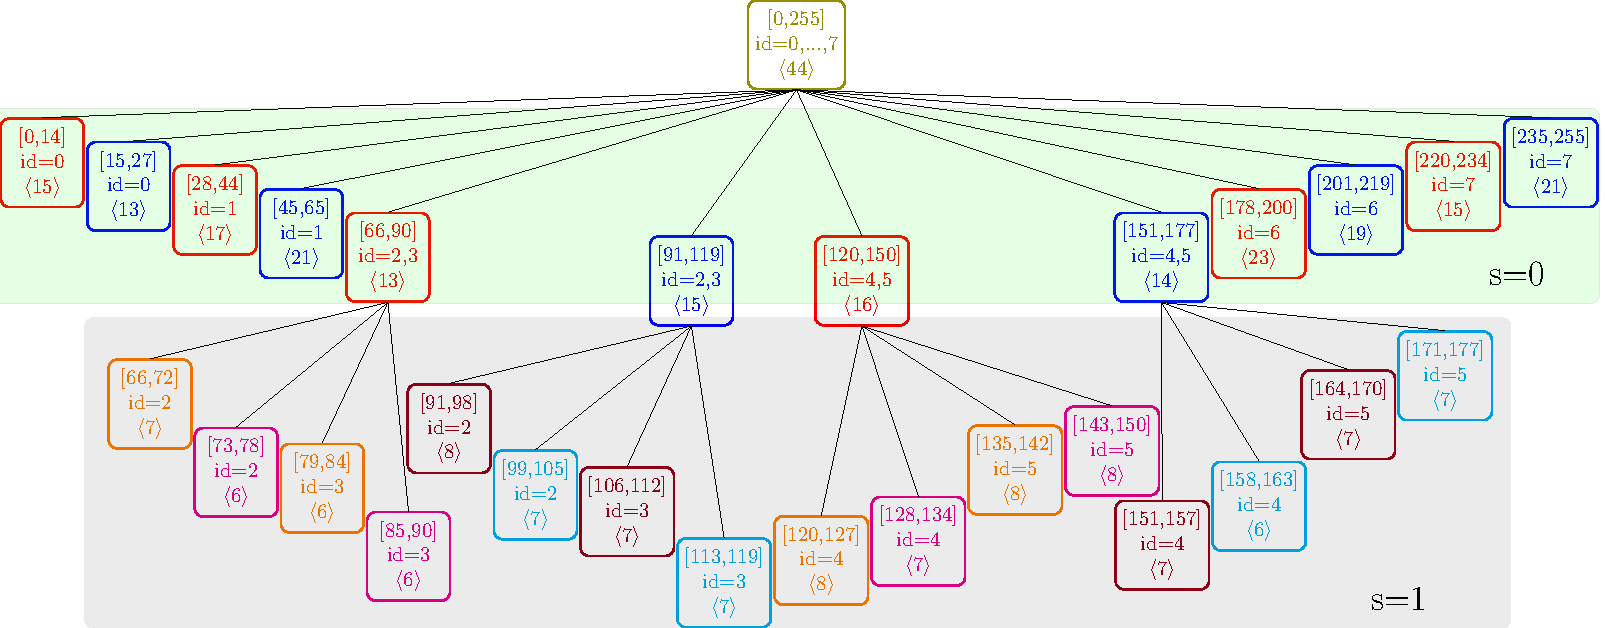
\includegraphics[width=\textwidth, height=0.2\textheight]{pics/recursion/2d-7pt_example/tree/tree}
	 	\caption{The internal tree structure of \acrshort{RACE} representing the \stex for domain size $16 \times 16$ and eight threads. The range $[\ldots]$ specified in each leaf represents the vertices belonging to each \levelGroup and the id refers to the thread id assigned to each \levelGroup assuming compact pinning . The last entry $\langle\acrshort{nrowsEff}\rangle$ gives the effective row number introduced in  \Cref{Sec:param_study}. }
	 	\label{fig:rec_2d-7pt_tree}
	 \end{figure}

\begin{comment}

{\GW Needs to be removed finally from here on till chapter 7}
%
%
%
While we achieved reasonable load balancing for the $16 \times 16$ \stex on five threads in ~\Cref{fig:2d_7pt_lb}, requesting parallelization for eight threads will lead to massive load imbalance due to the \DTWO coloring constraint: At least one thread operating on two inner successive levels has a load of 31 vertices, e.g. if it operates on levels 15 and 16. However, the optimal load per thread is 16 vertices in a single color restricting the parallel speed-up to four, i.e. the parallel efficiency to 50 \%. {\CA This example between 5 and 8 threads is for the necessity of recursion and does not clearly stress the importance of global load balancing. One idea to motivate the importance of global load balancing is by telling currently with recursion we have 2 ways of parallelism one within a stage by increasing level groups of a stage (horizontal parallelism) and second by recursion on a single level group to form level groups in next stage (vertical parallelism). Choosing the right combination of both these parallelism levels require a global load balancing scheme. Current load balancing scheme \Cref{subsec:LB} considers only the horizontal parallelism, now we have to extend it to incorporate also the vertical element of parallelism introduced by recursion.}

Thus, we have to modify/replace  {\GW Christie: can you comment on that (???)} {\CA (It is modification of the existing load balancing step, by allowing more threads per level group)} our original load balancing scheme {\CA{\sout{which assumed a single thread per \levelGroup}}}. {\CA The modification allows multiple threads to be assigned to a single level group $T_{s}(i)$ at stage $s$, threads that are assigned to specific level groups can then be spawned in the subsequent stages ($s+1, s+2, ...$) of recursion. The basic idea here is to assign multiple threads to \levelGroups containing bigger levels, and for simplicity we enforce equal number of threads to adjacent \levelGroups having different color.   To determine the number of threads responsible for a \levelGroup $T_{s}(i)$ following steps are followed:} 

\begin{enumerate}
	\item  First we assign weights to all levels in a specific stage ($s$) of the recursion. Assuming that $L_s(i) \subset T_{s-1}(j)$ its weight is defined by
	
	\begin{align*}
		w(L_s(i)) &= \frac{n_r(L_s(i))}{\frac{\nrowsMath^{total}}{\acrshort{nthreads}^{}}}=\frac{n_r(L_s(i))}{\nrowsMath^{total}}  {\acrshort{nthreads}^{}}\\
		\acrshort{nthreads} &: \text{total number of threads to be used for computing $T_{s-1}(j)$}\\
		\nrowsMath^{total} &= n_r(T_{s-1}(j)) %\text{, i.e. number of vertices in graph}
	\end{align*}
	In the initial stage ($s=0$) the base \levelGroup ($T_{-1}(0)$) is the full matrix/graph and $\acrshort{nthreads}$ is the total number of threads available. This weight describes which fraction of the optimal load per thread ($\frac{\nrowsMath^{total}}{\acrshort{nthreads}^{}}$)  is available in the specific level. 

	For the example shown in \Cref{fig:rec_2d-7pt_graph} requiring 8 threads ($T_{-1}(0) = 8$), weights would be 
	\begin{align*}
		\{w(L_0(0)), w(L_0(1)), w(L_0(2)), ...\} &= \{0.03125, 0.0625, 0.09375, ...\}
	\end{align*}
	
	\item The above definition of weight implies if the weight is close to a natural number $b$, the load induced by rows included in the calculation of weights is close to optimal for operation with $b$ threads. Thus starting with $L_s(0)$ we sum the weights till it forms a number $a$ close to a natural number $b$. Distance-k coloring is ensured by enforcing \atleast $2 \times k$ \levels in the sum, \ie for \DTWO coloring at least four levels (two for red and two for blue) are included. Closeness of the number is measured by a parameter $\epsilon$ defined as:
	\begin{align*}
		\epsilon &=  1 - abs(a-b)\\
		\text{where } b&= max(1,round(a))
	\end{align*}
	Closeness is controlled by the criteria:
	\begin{align*}
		\epsilon &> \epsilon_s, \text{where $\epsilon_s$ is a control parameter in the range of (0,1)} 	\end{align*}	
	   
	 Once we find a sum satisfying the criteria weight $b$ is fixed. Then we assign first \levelGroup of each color ($T_s(0)$ and $T_s(1)$) to be operated by $b$ threads. With fixed $b$ we try increasing levels in the \levelGroup to check if we can find a better natural number $a'$ closer to $b$ which would increase $\epsilon$ value, if found the new set is considered for allocating weights for $T_s(0)$ and $T_s(1)$. 
	 
	 Thus in case of our example in \Cref{fig:rec_2d-7pt_graph} with $\epsilon_s = 0.6$,  $w(L_0(0)) + w(L_0(1)) + ... + w(L_0(5)) = 0.65625$ satisfies the criteria $\epsilon = 0.65625 > \epsilon_s$, and $b=1$. Therefore one thread ($b=1$) is to be assigned for $T_0(0)$ and  $T_0(1)$. Now fixing $b=1$ we check increasing levels and finally find $w(L_0(0)) + w(L_0(1)) + ... + w(L_0(6)) = 0.875$ gives the highest $\epsilon$ value. Thus for constructing weights of $T_0(0)$ and $T_0(1)$ first 7 levels are used.
	
	\item Weights of subsequent \levelGroups ($T_s(2), T_s(3), ...$) are found by repeating the summing procedure starting with the very next \level. Finally once all the  levels are touched $\acrshort{nthreads}$ threads would be allocated between pairs (red and blue) of \levelGroups. 
	
	For example in case of \Cref{fig:rec_2d-7pt_graph} in order to find number of threads to be assigned for $T_0(2)$ and $T_0(3)$ we start summing from eighth level onwards ($w(L_0(7))$) and find one thread ($b=1$) satisfy the above criteria. For $T_0(4)$ and $T_0(5)$  two threads satisfy the criteria.
\end{enumerate}

Once all the weights are determined using this procedure a weighted load balancing scheme is employed. The scheme remains similar to the one seen in \Cref{subsec:LB} except while calculating mean and variance the weights are considered such that after load balancing ideally a \levelGroup with weight $w$ will have $w$ times more load (rows) than a \levelGroup with weight one. Same algorithm \Cref{alg:LB} presented in \Cref{subsec:LB} can be used except now the weights are the $b$ values instead of ones's. As explained previously in \Cref{subsec:LB} this also takes into account load balancing between different colors (red and blue).

%{\GW Christie: Please describe your scheme step by step with an itemize list and use examples from ~\Cref{fig:rec_2d-7pt_graph}}

    
	\subsubsection{TO BE SKIPPED Internal representation of recursively generated \boldmath{\levelGroups}} \label{subsec:level_tree}
	The recursive nature of our procedure allows to exploit more parallelism. However this introduces more complexity and one has to additionally respect the dependencies between stages and still observe the dependencies within one stage. The best idea is to have a data structure similar to the recursion, therefore we extent the \levelPtr data structure to a hierarchical tree data structure to store these informations. This data structure is called a \levelTree. The root of \levelTree contains information of entire domain, first child leaves of this root \ie leaves with depth 1 stores information about \levelGroups in first stage ($T_0(..)$), leaves with depth 2 stores information about \levelGroups in second stage ($T_1(...)$) and so on. 
	
 
 \Cref{fig:rec_2d-7pt_tree} shows a \levelTree corresponding to \stex  with 8 threads seen in \Cref{fig:rec_2d-7pt_graph}. The leaves in the tree correspond to different \levelGroups and store various informations like the range of vertices or the nodes that belong to this \levelGroup, the effective number of rows (\acrshort{nrowsEff}) that describes the quality of the method (which we will see later in \Cref{Sec:param_study}), and other informations like {\tt thread\_id} assigned to specific \levelGroups.  Threads are assigned to each \levelGroup depending on the pinning strategy used. For example in \emph{fill} type pinning strategy one would pin thread 0 to $T_0(0)$ and $T_0(1)$, thread 1 to $T_0(2)$ and $T_0(3)$, thread 2 to $T_1(0)  \subset T_0(4)$, $T_1(1) \subset T_0(4)$, $T_1(0)  \subset T_0(5)$ and $T_1(1) \subset T_0(5)$, and so on as seen in \Cref{fig:rec_2d-7pt_tree}. 
 
 Note that the \levelTree has a data structure that represents the nested parallelism being used as seen in \Cref{fig:rec_2d-7pt_graph} (right). Therefore threads are spawned based on this \levelTree allowing for easy implementation of point to point synchronizations.

\subsubsection{TO BE SKIPPED Sub-graph selection and global load balancing} \label{subsec:subgraph_selection_old}
Parallelism required for hardware underneath can be obtained either by expanding the \levelTree horizontally \ie increasing \levelGroups within a stage or by expanding \levelTree vertically with the help of recursion. But as we have seen before in \Cref{subsec:DK} the horizontal parallelism is limited by total levels (\acrshort{totalLvl}) and after a certain extent this would lead to load balancing problems. Similarly excessive usage of recursion is also not a good idea since data locality worsens due to local permutations within \subgraph. Therefore it is vital to find a proper balance and choose proper configuration. Furthermore just doing load balancing within a single stage is not the best, for example if we had equally balanced within stage 0 in \Cref{fig:rec_2d-7pt_tree}, we would receive no benefit from recursion. Therefore a global load balancing becomes inevitable.

\Inorder to select proper \subgraph and do global load balancing we employ a simple algorithm to find proper weights for each \levelGroup ($T_s(i)$) in a particular stage, then depending on this weights, denoted as $w(T_s(i))$, we do load balancing with weights in the particular stage $s$ (algorithm for this is similar to \Cref{alg:LB}, except weightage is given to \levelGroups). Finally if $w(T_s(i)) > 1$ we use recursion to achieve $w(T_s(i))$ parallel work in the next stage $T_{s+1}(i)$. The basic structure of the algorithm employed to find weights for the first stage is as follows:
\begin{enumerate}
	\item Find weights, $w(L_0(i))$ for each level in the current stage ($s$) by
		\begin{align*}
			w(L_0(i)) &= (\levelPtr_0[i+1] - \levelPtr_0[i])*\frac{\acrshort{nthreads}}{\nrowsMath^{total}}\\
			\acrshort{nthreads} &: \text{total parallelism required by hardware}\\
			\nrowsMath^{total} &: \text{number of vertices in graph}
		\end{align*}
	
	\item Starting from $w(L_0(0))$ sum up weights till they form a number ($a$) close to whole number ($b$). The closeness can be controlled by an efficiency parameter for stage $s$, $\epsilon_s$ is defined as:
	\begin{equation} \label{eq:epsilon}
		\epsilon_s =  1 - abs(a-b);
	\end{equation}
	All the \levels that are involved in the sum belongs to \levelGroups  operated by first thread in the current stage. The obtained number $b$ is chosen as weight for these \levelGroups \ie $w(T_0(0))=w(T_0(1))=b$. A local search is then done by increasing \levels in this \levelGroups to see if there is a better choice ($a$ close to $b$) with weight $b$, finally \levelGroups are formed with the best choice.  The weight for next \levelGroups are found by resetting the sum counter to zero and repeating the  procedure with \levels just after the current \levelGroups.
\end{enumerate}
For other recursive stage ($s\geq1$) same procedure can be applied to find weights $w(T_s(i))$, except that now $\acrshort{nthreads}$ and $\nrowsMath^{total}$ has to be substituted with the threads required and vertices in the \subgraph considered.

\end{comment}


\section{Parameter study}
\label{Sec:param_study}
% SIAM Shared Information Template
% This is information that is shared between the main document and any
% supplement. If no supplement is required, then this information can
% be included directly in the main document.

%In this section we study the impact of parameter $\epsilon_s$ and hardware parallelism on the quality of  \acrshort{RACE} method. \Inorder to do this we first quantify the quality of the method and finally we  use this quantity to do a parameter study. The study gives insights into tuning of parameter $\epsilon_s$ based on the given matrix and required parallelism.


The \acrshort{RACE} method introduced above has a set of input parameters $\{\epsilon_s; s=0,1,\ldots\}$ which controls the assignment of the number of threads to adjacent level groups. 
%For that reason a good choice is to have values close to $1$ for the initial stages and have a more relaxed constraint on the lower levels. 
To determine useful settings, we briefly analyze the interaction between these input parameters, the number of threads used, and the parallel efficiency of the generated workload distribution. 

As the internal tree structure contains all information about the final workload distribution, we can use it to identify the critical path in terms of workload and correspondingly the parallel efficiency. To do so we introduce the \effRow for every node (or \levelGroup) $\acrshort{nrowsEff}(T_s(i))$  which is a measure for the absolute runtime to calculate the corresponding \levelGroup. For \levelGroups which are not further refined (leaf nodes) this value is their actual workload, \ie the number of rows assigned to them ($\acrshort{nrowsEff}(T_0(0)) = 15$ in \cref{fig:rec_2d-7pt_tree}). For an inner node the \effRow  is the sum of the maximum workload (\ie max. \effRow value) across each of the two colors of its child nodes:

\begin{align*}
\acrshort{nrowsEff}(T_s(i)) &= max(\acrshort{nrowsEff}(T_{s+1}(j) \subset T_s(i))) + max(\acrshort{nrowsEff}(T_{s+1}(j+1) \subset T_s(i)))\\
 & \text{for } j=0,2,\ldots.
\end{align*}

Such a definition is based on the idea that nodes at a given stage $s$ have to synchronize with each other and have to wait for their siblings with the largest workload in each sweep (color). Propagating this information upwards on the tree until we reach the root node constructs the critical path in terms of longest runtime taking into account single thread workloads, dependencies, and synchronizations. Thus, the final value in the root node $\acrshort{nrowsEff}(T_{-1}(0))$ can be considered as the effective maximum workload of a single thread. Dividing the globally optimal workload per thread ($\frac{\acrshort{nrows}^{total}}{\acrshort{nthreads}}$) by this number gives the parallel efficiency ($\eta$) of our workload distribution: 

\begin{align*}
	\eta &= \frac{ \acrshort{nrows}^{total}} {\acrshort{nrowsEff}(T_{-1}(0)) \times \acrshort{nthreads}}. 
\end{align*}
For the tree presented in \cref{fig:rec_2d-7pt_tree} the parallel efficiency is limited to $\eta=\frac{256}{44 \times 8 } = 0.73$ on eight threads, \ie the maximum parallel speedup is $5.8$.

\subsection{Parameter analysis and selection}
\label{subsec:param_analysis}
The parallel efficiency (\acrshort{eta}) as defined above can be calculated for any given matrix, number of threads $\acrshort{nthreads}$,  and choice of $\{\epsilon_s; s=0,1,\ldots\}$ reflecting the quality of  parallelism generated by \acrshort{RACE} for the problem at hand.  This way we can understand the interaction between these parameters and identify useful choices for $\{\epsilon_s; s=0,1,\ldots\}$. Of course running a specific kernel such as \acrshort{SymmSpMV} on actual hardware will add other hardware and software constraints such as attainable memory bandwidth or cost of synchronization constructs. 

As a first step we can limit the parameter space by simple corner case analysis. Setting all parameters close to one requests high quality load balance but may prevent our load balancing scheme from termination. In the extreme case of $\{\epsilon_s=1; s=0,1,\ldots\}$ the scheme may generate only two \levelGroups (one of each color) in each recursion, assign all threads to them, and may further attempt to refine them the same way.  The lowest possible value of $\epsilon_s$ is the maximum deviation of a real number from its nearest integer which is 0.5. A range of  [0.5,0.9] for the $\epsilon_s$ values is therefore used in the following. For a basic analysis we have selected the \emph{inline} matrix (see \cref{tab:test_mtx}) as it has a rather small amount of parallelism and allows us to cover basic scenarios. In \cref{fig:inline_param_study}  we demonstrate the impact of different choices for $\epsilon_0$ and $\epsilon_1$ on the parallel efficiency for thread counts up to 100, which is a useful limit for modern CPU-based compute nodes. 
%
\begin{figure}[tbhp]
	\centering
	\subfloat[$\eta$ versus \acrshort{nthreads} for \emph{inline} matrix, $\epsilon_1 = 0.5$ ]{\label{fig:inline-a}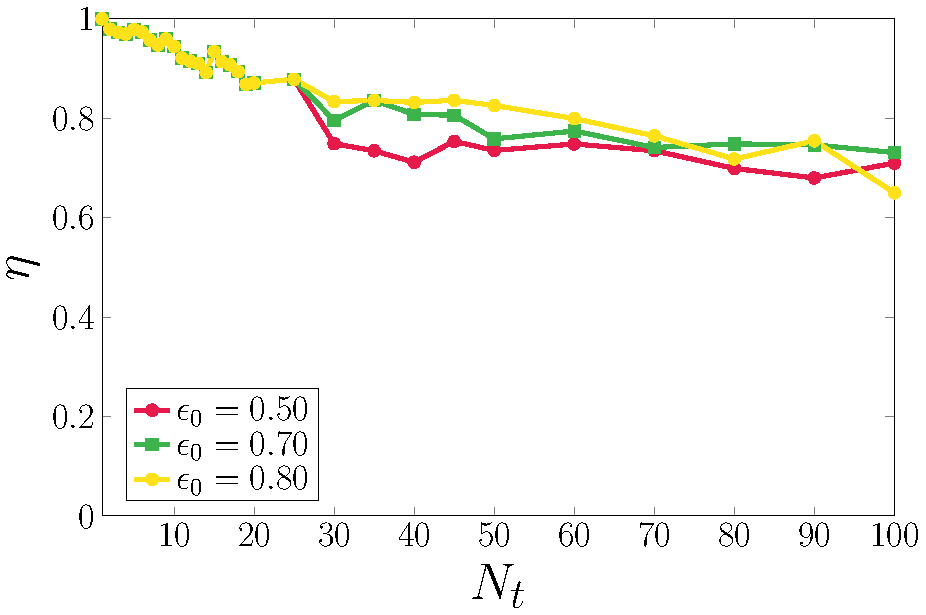
\includegraphics[width=0.45\textwidth , height=0.2\textheight]{pics/param_study/threads_vs_eff}}
	\hspace{1.5em}
	\subfloat[\acrshort{nthreads}=25]{\label{fig:inline-b}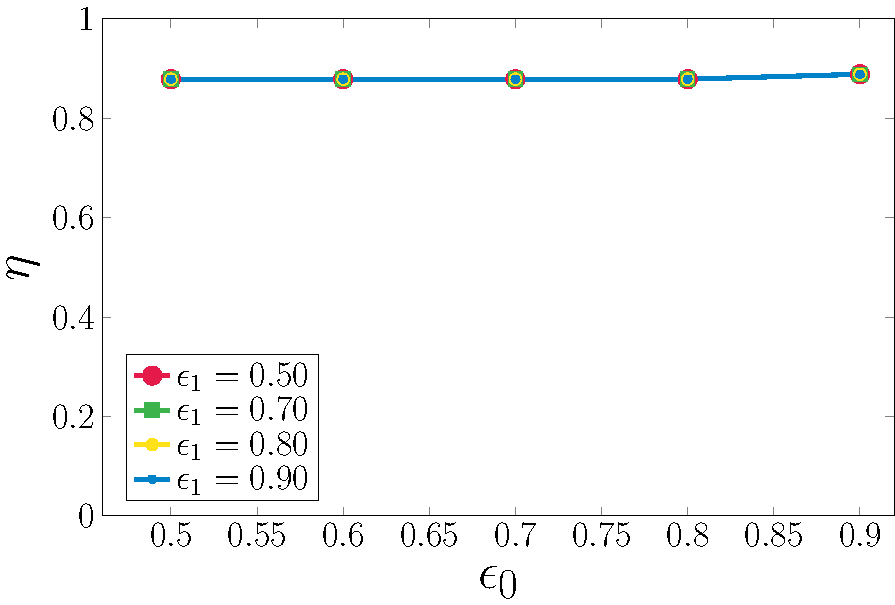
\includegraphics[width=0.45\textwidth , height=0.2\textheight]{pics/param_study/scaling_eps_1_25_threads}}
	
	\subfloat[\acrshort{nthreads}=45 ]{\label{fig:inline-c}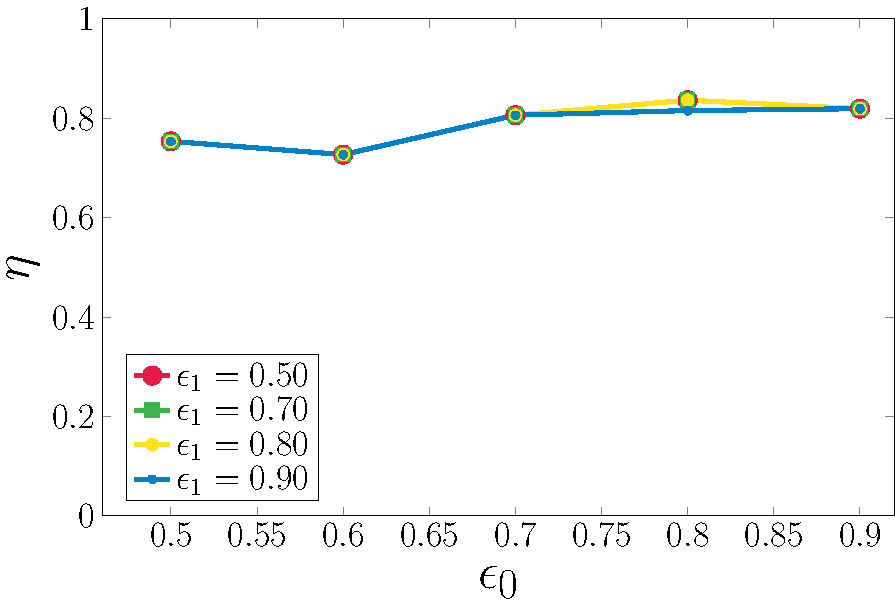
\includegraphics[width=0.45\textwidth , height=0.2\textheight]{pics/param_study/scaling_eps_1_45_threads}}
	\hspace{1.5em}
	\subfloat[\acrshort{nthreads}=100 ]{\label{fig:inline-d}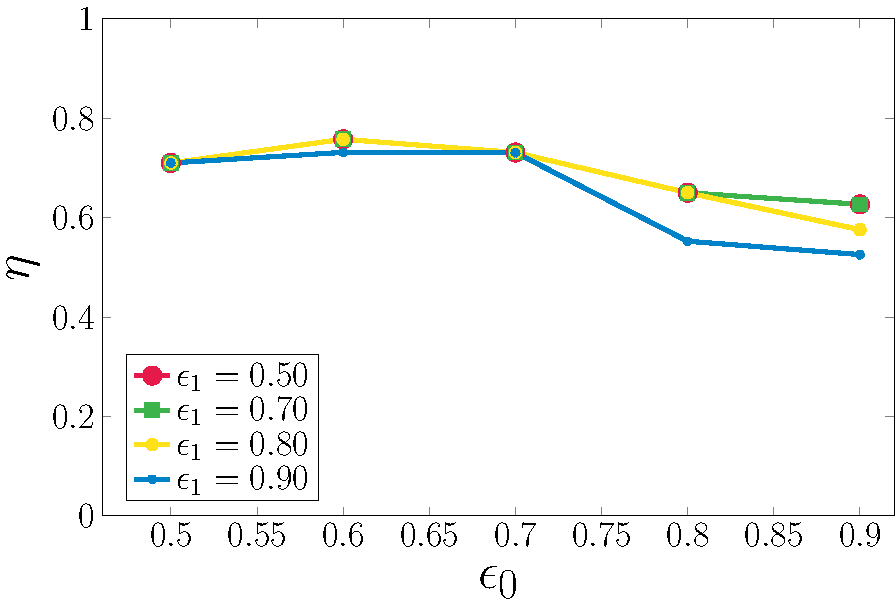
\includegraphics[width=0.45\textwidth , height=0.2\textheight]{pics/param_study/scaling_eps_1_100_threads}}
	\caption{Parameter study on \emph{inline} matrix. In \cref{fig:inline-b,fig:inline-c,fig:inline-d} each of the lines in the plot are iso-$\epsilon_1$ and impact of $\eta$ with respect to $\epsilon_0$ is shown. $\epsilon_s$ for $s>1$ is fixed to $0.5$.}
	\label{fig:inline_param_study}
\end{figure}
%
For $s > 1$ we always set the minimum value of $\epsilon_s=0.5$. The limited parallelism can be clearly observed from \cref{fig:inline-a}  with efficiency steadily decreasing with increasing thread counts. With a choice of $\epsilon_1=0.5$ there is only a minor impact of the parameter $\epsilon_0$. In \cref{fig:inline-b,fig:inline-c,fig:inline-d} the interplay between these two parameters is analyzed at different thread counts in more detail. We find that up to intermediate parallelism ($\acrshort{nthreads}=50$) the exact choice has only a minor impact on the parallel efficiency (see y-axis scaling). For large levels of parallelism the interplay becomes more intricate where too large values of $\epsilon_{0,1}$ may lead to larger imbalances. Based on this evaluation we choose $\epsilon_{0,1}=0.8$ and $\epsilon_s=0.5$ for $s>1$ for all the performance measurements. The quality of this choice in terms of parallel efficiency for all matrices is presented in \cref{fig:param_all_mtx_stat}. Here we plot the $\eta$ value for all the matrices over a large thread count. We find that our parameter setting achieves parallel efficiencies of 80\% or higher for a substantial fraction of the matrices up to intermediate thread counts. 
   \begin{figure}[tbhp]
   	\centering
   	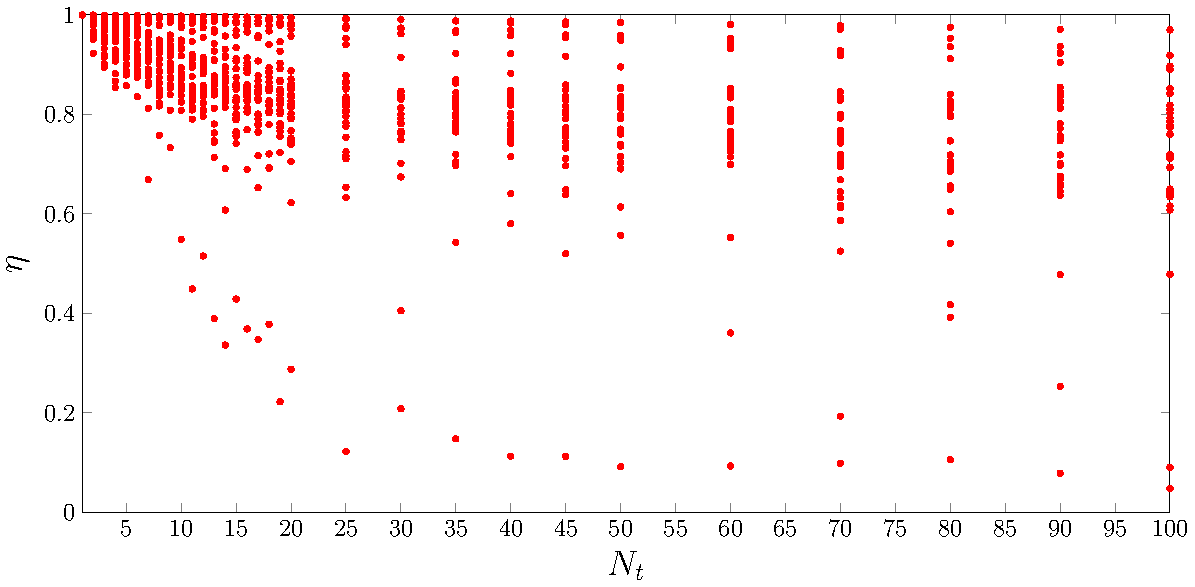
\includegraphics[height=0.19\textheight,width=0.9\textwidth]{pics/param_study/scatter_plot}
   	\caption{Scatter plot of $\eta$ versus \acrshort{nthreads} for all test matrices with $\epsilon_{0,1} = 0.8$ and $\epsilon_{s>1} = 0.5$.}
  	\label{fig:param_all_mtx_stat}
   \end{figure}
Representing the upper (lower) values in \cref{fig:param_all_mtx_stat} is the best (worst) case matrix \emph{Graphene-4096} (\emph{crankseg\_1}) exhibiting almost perfect (very low) parallel efficiencies at intermediate to high thread counts.

Finally, we evaluate the scalability of RACE using these two corner cases and the \emph{inline\_1} matrix as well as the \emph{parabolic\_fem} matrix, which is small enough to fit into the cache. 
In \cref{fig:corner_cases_param} we basically mimic scaling tests on one Skylake processor with up to 20 cores (\ie threads) and plot the parallel efficiency $\eta$ as well as the maximum number of threads which can be ``perfectly'' used \acrshort{threadEff} (\ie $\acrshort{threadEff} = \eta*\acrshort{nthreads}$). 
%
\begin{figure}[tbhp]
	\centering
	\subfloat[\emph{crankseg\_1}]{\label{fig:crankseg_param}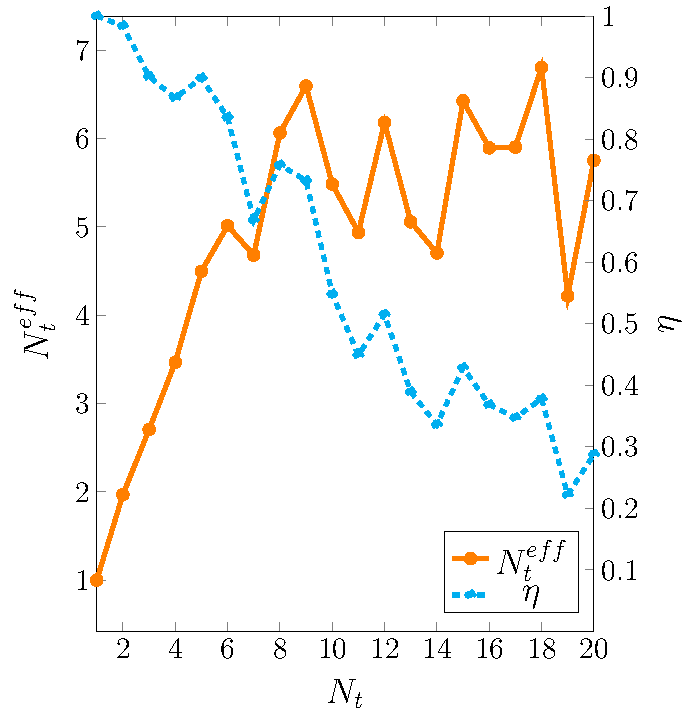
\includegraphics[width=0.23\textwidth , height=0.16\textheight]{pics/param_study/corner_cases/crankseg_1}}
	\subfloat[\emph{inline\_1}]{\label{fig:inline_param}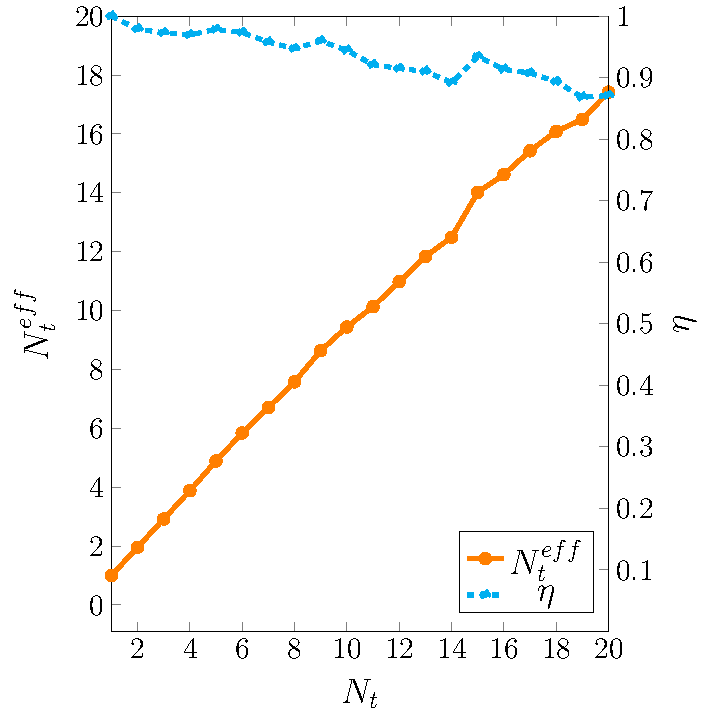
\includegraphics[width=0.23\textwidth , height=0.16\textheight]{pics/param_study/corner_cases/inline_1}}	
	\subfloat[\emph{parabolic\_fem}]{\label{fig:parabolic_fem_param}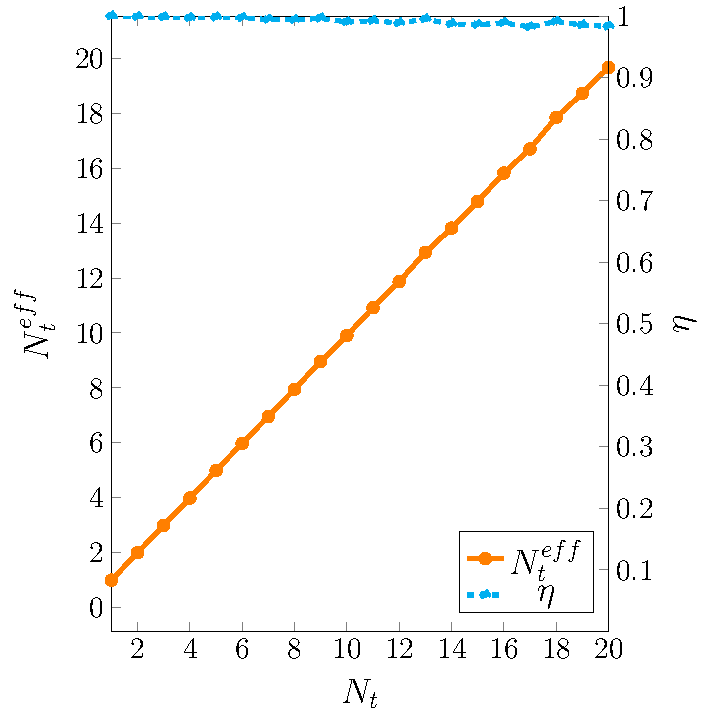
\includegraphics[width=0.23\textwidth , height=0.16\textheight]{pics/param_study/corner_cases/parabolic_fem}}
	\subfloat[\emph{Graphene-4096}]{\label{fig:Graphene-4096_param}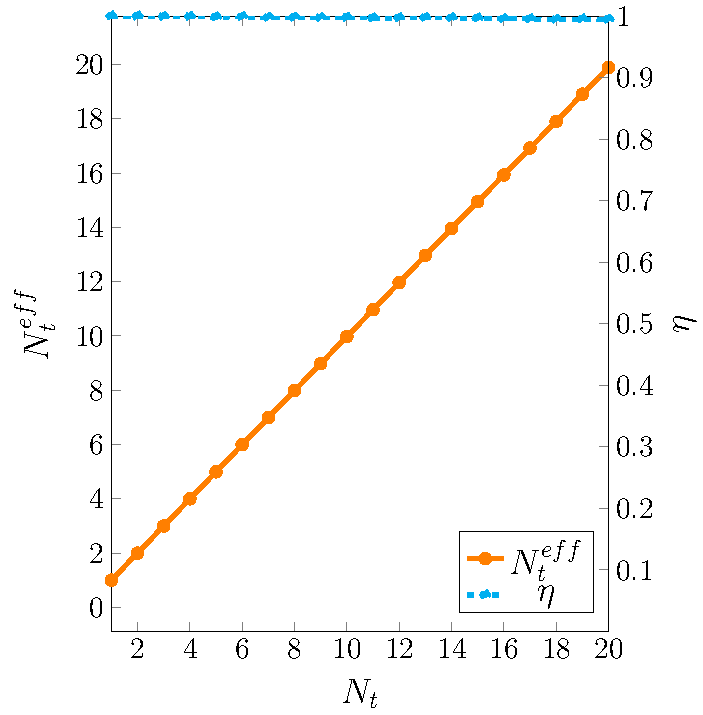
\includegraphics[width=0.23\textwidth , height=0.16\textheight]{pics/param_study/corner_cases/Graphene-4096}}	
	\caption{\acrshort{threadEff} and $\eta$ versus \acrshort{nthreads} for the four corner case matrices, with the same settings used in experiment runs. \acrshort{threadEff} is defined as $\eta$ * \acrshort{nthreads}.}
	\label{fig:corner_cases_param}
\end{figure}

\begin{figure}[tbhp]
	\centering
	\subfloat[\emph{crankseg\_1}]{\label{fig:crankseg_scaling}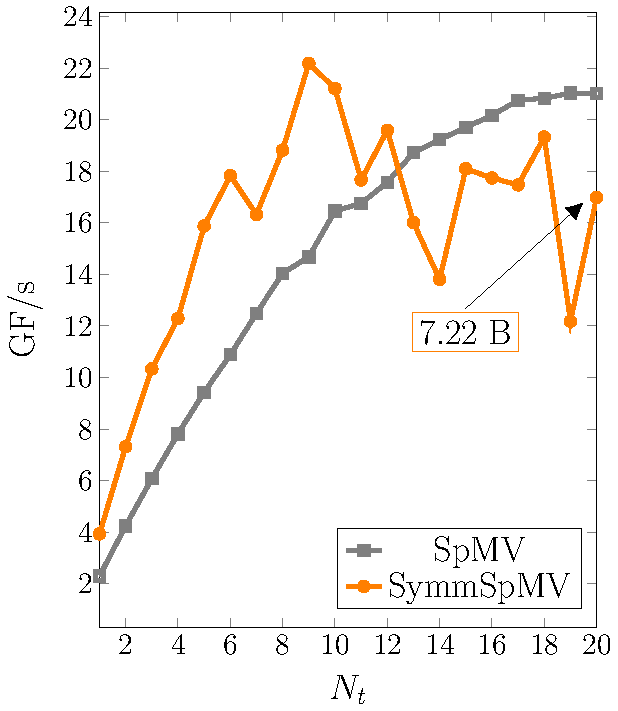
\includegraphics[width=0.23\textwidth , height=0.18\textheight]{pics/results/skx/corner_cases_scaling/plots/RCM/crankseg_1_RCM}}
	\subfloat[\emph{inline\_1}]{\label{fig:inline_scaling}\includegraphics[width=0.23\textwidth , height=0.18\textheight]{pics/results/skx/corner_cases_scaling/plots/RCM/inline_1_RCM}}	
	\subfloat[\emph{parabolic\_fem}]{\label{fig:parabolic_fem_scaling}\includegraphics[width=0.23\textwidth , height=0.18\textheight]{pics/results/skx/corner_cases_scaling/plots/RCM/parabolic_fem_RCM}}
	\subfloat[\emph{Graphene-4096}]{\label{fig:Graphene-4096_scaling} \includegraphics[width=0.23\textwidth , height=0.18\textheight]{pics/results/skx/corner_cases_scaling/plots/RCM/Graphene-4096_RCM}}	
	\caption{Parallel performance measurements of \acrshort{SymmSpMV} with \acrshort{RACE} on one socket of \SKX architecture for the four corner case matrices. For comparison, the performance of the basic \acrshort{SpMV} kernel is presented. For the matrices \cref{fig:inline_scaling,fig:parabolic_fem_scaling,fig:Graphene-4096_scaling} the maximum roofline performance limits \cref{eq:upper_performance} are given using the computational intensity \cref{eq:SymmSpMV_intensity} for the two extreme cases of load only memory bandwidth (RLM-load) and copy memory bandwidth (RLM-copy). The measured full socket main memory data traffic per nonzero entry (in \mbox{B}/\acrshort{nnz}) is also shown. }
	\label{fig:corner_cases_scaling}
\end{figure}

The unfavorable structure of the \emph{crankseg\_1} matrix puts strict limits on parallelism even for low thread counts.  The combination of small matrix size with a rather dense population (see \cref{table:bench_matrices}) leads to large inner levels when constructing the graph triggering strong load imbalances if using more than six threads. Searching for better $\epsilon_s$ slightly changes the characteristic scaling but not the maximum parallelism which can be extracted. For the \emph{inline} matrix we find a weak but steady decrease of the parallel efficiency which is in good agreement with the discussion of \cref{fig:inline_param_study}. The other two matrices scale very well in the range of thread counts considered. 

The corresponding performance measurements for the \acrshort{SymmSpMV} kernel (see \cref{sect:SymmSpmv}) on a single \SKX processor chip with 20 cores are shown in \cref{fig:corner_cases_scaling}. \footnote{For the benchmarking setup see \cref{Sec:expt}.} 
%A strong relationship between the theoretical  (\cref{fig:corner_cases_param}) and  experimental (\cref{fig:corner_cases_scaling}) scaling graph can be clearly observed. 
For the \emph{crankseg\_1} matrix (see \cref{fig:crankseg_scaling}) we recover the limited scaling due to load imbalance as theoretically predicted. A performance maximum is at nine cores where the maximum \acrshort{SpMV} performance can be slightly exceeded. However, based on the roofline performance model given by \cref{eq:SymmSpMV_intensity,eq:upper_performance}, together with the matrix parameters from \cref{table:bench_matrices}, a theoretical speedup of approximately two as compared to \acrshort{SpMV} can be expected for the full processor chip. 
In the case of \emph{inline\_1} and \emph{Graphene-4096} matrices we find good agreement with the theoretical considerations. Performance scales almost linearly until we hit the main memory bandwidth bottleneck and the saturated performance numbers are in good agreement with the roofline performance limits.  
%although the experimental and theoretical results match for the initial phase it shows a different behavior towards the end. This happens since the kernel saturates the memory bandwidth available for this chip, which can be easily verified by observing the close agreement of the full socket performance and the performance model prediction given by \cref{eq:SymmSpMV_intensity,eq:upper_performance}. 
It should be noted that even though \emph{inline\_1} matrix didn't have theoretically perfect efficiency ($\eta$ $\approx 0.85$ at $\acrshort{nthreads}=20$), it still generates sufficient parallelism to achieve main memory saturation. 
%The only affect of the lower efficiency was a shift in saturation point to further right (at higher thread count) compared to \emph{Graphene-4096}. 
The good agreement of theoretical and experimental results for  \emph{parabolic\_fem}  (see \cref{fig:parabolic_fem_param,fig:parabolic_fem_scaling}) is due to the fact that it is small ($\approx 23$ \MB) enough to fit into caches of the Skylake processor (\acrshort{LLC} size $= 28$ MB). Thus, performance is not limited by main memory bandwidth constraint and the roofline model limits do not apply.

We have demonstrated that a simple choice for the only set of RACE input parameters $\{\epsilon_s; s=0,1,\ldots\}$ can extract a sufficient amount of parallelism for most matrices considered in this study. Moreover, the parallel efficiency as calculated by RACE in combination with the roofline performance model is a good indication for scalability and maximum performance of the actual computations.

\begin{comment}
\subsection{Corner Cases}



\Cref{fig:corner_cases_scaling} shows the scaling performance of \acrshort{SymmSpMV} and \acrshort{SpMV} (baseline) kernel for corner case matrices on one socket of \SKX architecture. Chosen corner case matrices represent different aspects and bottlenecks that appear either due to \acrshort{RACE} method or because of hardware capabilities.

The \emph{crankseg\_1} matrix is the worst in terms of performance. It does not scale well due to it's limited parallelism obtained using the \acrshort{RACE} method. This property of \emph{crankseg\_1} is well evident directly after doing the theoretical estimate based on $\eta$ as  seen in \cref{fig:crankseg_param}. One could further see that the actual scaling run of the kernel seen in \cref{fig:crankseg_scaling} is exactly in tune with that of the theoretical result. Note that due to this bottleneck of parallelism we didn't achieve much benefit from using \acrshort{SymmSpMV} compared to \acrshort{SpMV}.

The \emph{inline\_1} matrix although being third lowest in terms of parallelism in the entire set of test matrices, but it still achieves a high efficiency ($\eta$ = 0.85) for 20 threads (see \cref{fig:inline_param}), leading to good scaling as seen in \cref{fig:inline_scaling}. The saturation in performance after 15 threads is due to the fact that we hit the memory bottleneck, similar saturation behavior can also be observed for \acrshort{SpMV} which is embarrassingly parallel. The saturation occurs at the maximum achievable performance on the given architecture which could easily be verified using the \roofline model \cite{Williams_roofline} and intensity equations (see \cref{subsec:test_kernels}) as shown below:
\begin{align*}
	% P_{max} =&  2 \fracUnit{FMA AVX-512 instruction}{cy*cores}  * 8 \fracUnit{FMA}{FMA AVX-512 instruction} \\
	% & * 2 \fracUnit{Flop}{FMA} * 2.4 \fracUnit{Gcy}{s} * 20 \unit{cores} = 1536  \fracUnit{GFlop}{s} \\	 
	I_\mathrm{\acrshort{SpMV}} &= \frac{2}{8+4+\frac{8+16}{73}} = 0.162 \fracUnit{Flop}{byte} \text{, assuming best case : $\alpha = \frac{1}{\acrshort{NNZR}}$}\\
	P_\mathrm{\acrshort{SpMV}} &= b_s*I_\mathrm{\acrshort{SpMV}}; \text{  for memory-bound case}\\
	P_\mathrm{\acrshort{SpMV}} &= 0.162\fracUnit{Flop}{Bytes}*115\fracUnit{GByte}{s} = 18.6 \fracUnit{GFlop}{s}\\
\end{align*}

As seen we achieve 17.8 GFlop/s which is close to the theoretical maximum of 18.6 GFlop/s for \acrshort{SpMV}. Similar derivation can be done for \acrshort{SymmSpMV} and one could see $P_\mathrm{\acrshort{SymmSpMV}}$= 34.5 GFlop/s, which is approximately twice that of \acrshort{SpMV} since $I_\mathrm{\acrshort{SymmSpMV}}$ is almost a factor two higher than $I_\mathrm{\acrshort{SpMV}}$ for matrix with moderate \acrshort{NNZR} (see \cref{eq:SpMV_intensity,eq:SymmSpMV_intensity}). From \cref{fig:inline_scaling} one can observe that at saturation we reach close to theoretical values. A cushioning effect due to memory bandwidth bottleneck is also evident from \cref{fig:inline_scaling}, where we see that due to this saturation decrease in $\eta$ to a certain extent would not effect the socket level performance, it would just shift the knee of saturation towards right.

In the case of \emph{parabolic\_fem} matrix we theoretically have a good efficiency as seen from \cref{fig:parabolic_fem_param}, but here we do not see any saturation in performance (see \cref{fig:parabolic_fem_scaling}), even \acrshort{SpMV} does not have this saturation behavior. If one calculates the maximum  theoretical performance by \roofline model and assuming memory-boundedness as shown in previous example one would see that $P_\mathrm{\acrshort{SpMV}}$=15 GFlop/s and $P_\mathrm{\acrshort{SymmSpMV}}$=19 GFlop/s, but we achieve more than these values in actual runs 26.5 and 31.5 GFlop/s respectively. This is because the matrix is small enough ($\approx$ 46 MB for full matrix and $\approx$ 23 MB for symmetric storage) to just fit in caches (combined L2 and L3) of the \SKX architecture. Since the caches scales well on this architecture we don't observe the saturation behavior. It should be noted that in this case comparison between \acrshort{SpMV} and \acrshort{SymmSpMV} cannot be done directly since for \acrshort{SpMV} the total data is almost close to cache limits, while for \acrshort{SymmSpMV} it would easily fit in cache.

\emph{Graphene-4096} matrix on the other hand is a matrix with efficiency similar to \emph{parabolic\_fem} but with much larger size ($\approx 2 GB$) resulting in matrix data always coming from main memory. This therefore shows dominant saturation behavior and since we achieve good efficiency ($\eta$) the knee of saturation begins at a well early stage for \acrshort{SymmSpMV} compared to  the case of \emph{inline\_1} where the efficiency was lower in comparison resulting in smaller \acrshort{threadEff}.

\end{comment}

\begin{comment}
Quantifying quality of the method in a well-defined way is a primary and most vital step for parameter study. We do this using the concept of \effPar. From \cref{Sec:race} we saw that even though one tries to achieve parallelism exactly as that required by the hardware, in practice one might not be able to utilize this parallelism to 100 \% due to load imbalances. Therefore we use a simple calculation based on the \levelTree to determine efficiency. This takes into account load imbalances incurred from different stages of recursion. We first calculate \effRow for each of the worker leaves (leaves in finest level) in \levelTree.
The \levelGroups (leaves) in \levelTree that are not further refined form worker leaves and they are responsible for executing the rows (nodes) in their range, the work done by these leaves is therefore directly proportional to the number of rows. Hence the \effRow of these worker leaves is same as number of rows (\acrshort{nrows}), for example in case of $T_0(0)$ \effRow ( $\acrshort{nrowsEff}(T_0(0))$ = $\acrshort{nrows}(T_0(0))$ ) is 14 and $\acrshort{nrowsEff}(T_1(0) \subset T_0(4))$ is 6. After calculating the \effRow for worker leaves the information is propagated to other leaves in lower stages (up in the \levelTree) as follows: 
\begin{align*}
\acrshort{nrowsEff}(T_s(i)) &= max(\acrshort{nrowsEff}(T_{s+1}(j) \subset T_s(i))) + max(\acrshort{nrowsEff}(T_{s+1}(k) \subset T_s(i)))\\
 & \text{for } j \text{ is even and } k \text{ is odd}
\end{align*}

Such a definition for \effRow is based on the idea that a parent has to wait until the child leaf with most number of rows in each sweep (color) has finished it's work due to synchronization needed with it's siblings. This has to be handled separately for each of the two parallel sweep (colors) as there is this synchronization happening after each of the sweeps (colors). 

Once the information is propagated up the tree and as it reaches the root we have a single \effRow ($\acrshort{nrowsEff}(T_{-1})$) for the entire tree, which has taken into account load imbalance happening between all \levelGroups in all stages. The ratio of total number of rows ($\acrshort{nrows}^{total}$) in the entire matrix to that of $\acrshort{nrowsEff}(T_{-1})$ gives \effPar, denoted as \acrshort{threadEff}. Efficiency ($\eta$) of the method is then defined as ratio of  \acrshort{threadEff} to that of required hardware parallelism (\acrshort{nthreads}). 

\begin{align}
	\acrshort{threadEff} &= \frac{\acrshort{nrows}^{total}}{\acrshort{nrowsEff}(T_{-1})} \\
	\eta &= \frac{\acrshort{threadEff}}{\acrshort{nthreads}} \label{eq:eta}
\end{align}

For example in our \stex, \cref{fig:rec_2d-7pt_tree} shows \acrshort{nrowsEff} for each leaves in angular brackets and here $\acrshort{threadEff} = 5.8$ and $\eta = 0.725$. The value of $\eta = 1$ implies there is perfect load balancing which is almost impossible. In general $0 < \eta \leq 1$. This parameter $\eta$ will be used as a measure of quality in parameter study.

\subsection{Case study}
A given matrix has a fixed amount of parallelism and as the amount of required parallelism (\acrshort{nthreads}) increases load balancing degrades due to more threads per stage and imbalances between stages. The rate of degradation can however be controlled to certain extent by the tolerance $\epsilon_s$ (see \cref{eq:epsilon}) specified while choosing a \levelGroup. Typical value of $\epsilon_s$ is in range of [0.4,0.9]. Having a small $\epsilon_s$ (for example 0.4) implies we utilize the current stage `s' to maximum and do not impose high load balancing constraint, a high value on the other hand requires more balanced load from current stage `s'. 

Test matrices (see \cref{Sec:test_bed}) considered have a varying degree of parallelism, and in order to see the effect of $\eta$ and $\epsilon_s$ we choose the \emph{inline} matrix. The choice is due to the fact that this matrix has relatively small amount of parallelism and this allows us to demonstrate various effect, ranging from good to bad case scenario with small number of parallelism (\acrshort{nthreads}$ < 200$). This limited parallelism can be observed from \cref{fig:inline-a} 
where efficiency keeps on decreasing with \acrshort{nthreads} for \emph{inline} matrix. Similar behavior can be observed for \emph{crankseg\_1}, \emph{F1} and \emph{ship} matrices, of which \emph{crankseg\_1} being the worst. For majority of other test matrices one could observe that efficiency $\eta$ initially drops but then remains almost constant in the range $\eta$ = [0.50,0.80] (depending on matrix) for the entire scanned area of $1 \leq $\acrshort{nthreads}$ \leq 200$.

%\begin{figure}[tbhp]
%	\centering
%	\subfloat[$\eta$ vs \acrshort{nthreads} for \emph{inline} matrix ]{\label{fig:inline-a}\includegraphics[width=0.45\textwidth , height=0.2\textheight]{pics/param_study/threads_vs_eff}}
%	\hspace{1.5em}
%	\subfloat[Effect of $\epsilon_0$ at low \acrshort{nthreads}, \acrshort{nthreads}=25]{\label{fig:inline-b}\includegraphics[width=0.45\textwidth , height=0.2\textheight]{pics/param_study/scaling_eps_1_25_threads}}
%	
%	\subfloat[Optimal $\epsilon_0$ lowered and optimal $\epsilon_1$ = 0.9, \acrshort{nthreads}=45 ]{\label{fig:inline-c}\includegraphics[width=0.45\textwidth , height=0.2\textheight]{pics/param_study/scaling_eps_1_45_threads}}
%	\hspace{1.5em}
%	\subfloat[Optimal $\epsilon_0$ lowered to 0.4 and $\epsilon_1$ to 0.7, \acrshort{nthreads}=100 ]{\label{fig:inline-d}\includegraphics[width=0.45\textwidth , height=0.2\textheight]{pics/param_study/scaling_eps_1_100_threads}}
%	\caption{Parameter study on \emph{inline} matrix. In \cref{fig:inline-b,fig:inline-c,fig:inline-d} each lines in the plot are iso-$\epsilon_2$ and impact of $\eta$ with respect to $\epsilon_1$ is shown.}
%	\label{fig:inline_param_study}
%\end{figure}

At small number of threads (\acrshort{nthreads}) all matrices have high efficiency (like $\eta>0.8$). As there is a lot of parallelism in this stage compared to requirement, $\eta$ is insensitive of $\epsilon_s$. The value of \acrshort{nthreads} upto which such a behavior can be observed varies from matrix to matrix, for example \emph{inline} shows this upto \acrshort{nthreads}$\approx20$, while for matrix like \emph{Graphene} this is grater than $200$.  Further increasing \acrshort{nthreads} one could observe $\eta$ starts to vary with $\epsilon_0$. For example in case of \acrshort{nthreads}$ = 25$ one could see in \cref{fig:inline-b} maximum $\eta$ is achieved with high value of $\epsilon_0$ (0.9) due to good load balancing. But as 
\acrshort{nthreads} further increase the optimal $\epsilon_0$ starts shifting towards left (see \cref{fig:inline-c}),
 since one requires more parallelism from the current stage (s=0) and higher $\epsilon_0$ would be decremental since it would require the \levelTree to go more deep and hence load imbalances in next stages will get multiplied. $\epsilon_1$ which till now didn't effect much starts to influence slowly as \acrshort{nthreads} increments again, for example in case of \emph{inline} till $\acrshort{nthreads}=90$ $\epsilon_1=0.9$ was optimal, but then the optimal $\epsilon_1$ reduces and reaches $0.7$ at \acrshort{nthreads}$=190$ as seen in \cref{fig:inline-d}. $\eta$ would start to get affected by $\epsilon_s$ of next stages in similar manner with increase of \acrshort{nthreads}.
 
Behavior of other matrices in the test bed follow similar pattern, but \acrshort{nthreads} at which different phases occur varies from matrix to matrix.  \Cref{fig:param_all_mtx_stat} gives a broad overview of the efficiency ($\eta$) behavior of entire test matrices using scatter plot. Each point at a specific \acrshort{nthreads} represents efficiency ($\eta$) of a matrix. Majority of test matrices having an initial drop in $\eta$ and then remaining constant is reflected in the statistical plot. The lowest points in the plot correspond to \emph{crankseg\_1} matrix, here we achieve only a mere parallelism of eight at maximum (\acrshort{threadEff} = 8), while the upper points correspond to matrix having highest parallelism namely \emph{Graphene} matrix.

In practice for a given matrix it's difficult to precisely determine the optimal rate of decrease in $\epsilon_s$ without parameter search, and therefore selecting proper $\epsilon_s$ for given \acrshort{nthreads} can be challenging. One idea is to see total levels (\acrshort{totalLvl}) and distribution of nonzeros (\acrshort{nnz}) in different levels of current stage `s' and heuristically determine $\epsilon_s$ based on the pressure of parallelism from stage `s'. This is not currently done and is part of our future work. As a rule of thump an $\epsilon_{0,1} = 0.8$ and $\epsilon_{s>1} = 0.4$ is sufficient for most matrices on current architectures, therefore currently for experiments we set these $\epsilon_s$ values for all matrices.

 In \cref{fig:corner_cases_param} we have plotted \acrshort{threadEff} and $\eta$ vs \acrshort{nthreads} for corner case matrices with the settings used in experiment runs. Here we set $\epsilon_{0,1}=0.8$ and use \acrfull{RCM} in the \emph{level construction} stage (\cref{subsec:LEVEL_CONST}). Big fluctuation in \emph{crankseg\_1} is due to the fact that we set high load balancing requirement (high $\epsilon_s$ factor) and as seen in the example of \emph{inline\_1} matrix this is not optimal when we reach the limit of parallelism. The theoretical estimates obtained in \cref{fig:corner_cases_param} will be directly used to compare with experiment runs in the next section (\cref{Sec:expt}).

\end{comment}

\section{Performance Evaluation of \NoCaseChange{\acrshort{SymmSpMV}} using \acrshort{RACE}}
\label{Sec:expt}
% SIAM Shared Information Template
% This is information that is shared between the main document and any
% supplement. If no supplement is required, then this information can
% be included directly in the main document.


Our method has been implemented and consolidated into a library named \acrshort{RACE}. The library provides easy interface for parallelizing kernels having dependencies, user typically just needs to supply a callback function with the serial code (potentially with dependency) and specify the required hardware settings. Library will then parallelize and run the code in parallel. The library is made publicly available through the git repository.  %TODO
 
 In the following we present the results of two important benchmarks which makes use of the \acrshort{SymmSpMV} and \acrshort{SymmKACZ} kernels. The benchmarks are carefully constructed to mimic the actual settings in real application runs. These benchmarks results are further compared with current state of art alternative methods.
 
 Both the benchmarks are run on the full set of test matrices (see \cref{table:bench_matrices}) and the matrices are preprocessed with \acrshort{RCM} bandwidth reduction using the \SPMP library \cite{SpMP}.

\subsection{Benchmark - \acrshort{SymmSpMV}}
Sparse matrix vector multiplication is a frequently used operator in plenty of sparse numerical algorithms and is commonly the most time consuming one. This simple benchmark performs multiplication of a symmetric matrix with a vector, and involves a direct use of the \acrshort{SymmSpMV} kernel.  In this benchmark we store only the upper triangular part of the symmetric matrix and perform the full matrix vector multiplication as shown in \cref{sect:SymmSpmv}. 

The main purpose of the benchmark is to study the performance quality of the \acrshort{RACE} library and make a solid performance-only comparison between different methods due to the exact nature of the \acrshort{SymmSpMV} kernel.

\subsubsection{Test setup}
\Inorder to have well reproducible result and accurate timing measurements it is necessary to have multiple runs of the kernel. But running the same matrix vector multiplication over the same vectors could lead to caching of the vectors if the sizes are small enough. However this effect does not appear in actual practice since normally a matrix vector multiplication is followed by different calls to other kernels (commonly Level 1 BLAS) that in addition use other helper data leading to eviction of the cached vectors. To replicate this behavior we use two ring buffers holding vectors of size \acrshort{nrows}. Number of vectors in the buffer is chosen such that the combined size of both the ring buffer is \atleast 100 \MB, which is \atleast two times bigger than 
the combined cache sizes of both the architectures. The \acrshort{SymmSpMV} kernel is then run over these two buffers taking one vector each as input ($x$) and output vector ($b$) for the matrix vector operation ($b=Ax$). The kernel is run two times through all of the elements in this ring buffer and the mean performance of the runs is taken into account.

\begin{figure}[tbhp]
	\centering
	\includegraphics[scale=0.5]{pics/results/symm_spmv_setup/test_setup}
	\caption{Benchmark \acrshort{SymmSpMV} test setup}
\end{figure}
{\GW Will continue here...}

\subsection{Test setup}
In the following we present the performance and convergence results obtained using the library, and compare it against state of art methods. \acrshort{SymmSpMV} and \acrshort{SymmKACZ} are chosen as representative benchmark kernels. Hardware and matrices as described in \cref{Sec:test_bed} is used for the following benchmarks. As mentioned in \cref{Sec:param_study} parameter $\epsilon_s$ is set to 0.8 and \acrshort{RCM} is used in level construction stage. The matrix is pre-processed with \acrshort{RCM} for all the cases (even for \acrshort{SpMV}). \SPMP \cite{SpMP} library was used to do this \acrshort{RCM} pre-processing.

The test setup is so constructed that it replicates the behavior of these kernels in actual practical scenarios. Normally matrix vector multiplication is followed by different calls to other kernels that use other helper data. This may lead to eviction of residual data from matrix vector multiplication. In order to replicate this behavior for \acrshort{SymmSpMV} and \acrshort{SpMV} (used as reference) we use  two ring buffers holding vectors of size \acrshort{nrows}. Number of vectors in this ring buffer is chosen such that these two ring buffer occupy a size of 100 \MB, which is at least two times bigger that the combined cache size of the two architectures considered. The kernels are then run two times over these ring buffer, and mean performance of the runs is taken into account.

For \acrshort{SymmKACZ} there are two use cases. In one it is used as a plain iterative solver where the kernel is called successively. The other use case of this iterative solver is in algorithms like CGMN~\cite{CGMN, CGMN_gordon} or CARP-CG~\cite{CARP-CG} where \acrshort{SymmKACZ} is used like a preconditioner, where an approach similar to \acrshort{SymmSpMV} have to be used for benchmarking. In this paper the benchmark is constructed to replicate the behavior of the former case, \ie we call the \acrshort{SymmKACZ} kernel 500 times in succession and report the mean performance. It has to be noted that the difference in performance measurements between these two benchmarks is very small and only affects small matrices.


\subsection{Performance and comparisons}

\begin{figure}[thbp]
	\centering
	\subfloat[Comparison of \acrshort{SpMV} and \acrshort{RACE} \acrshort{SymmSpMV} on 1 socket of \IVB]{\label{fig:spmv_vs_symm_spmv_ivy}\includegraphics[width=0.85\textwidth, height=0.27\textheight]{pics/results/ivy/data_symm_spmv/plot_generator/perf_vs_mtx_RACE_w_SpMV/perf}}
	\hspace{1em}
	\subfloat[\acrshort{SymmSpMV} on 1 socket of \SKX]{\label{fig:spmv_vs_symm_spmv_skx}\includegraphics[width=0.85\textwidth, height=0.27\textheight]{pics/results/skx/data_symm_spmv/plot_generator/perf_vs_mtx_RACE_w_SpMV/perf}}
	\caption{\acrshort{SpMV} vs RACE \acrshort{SymmSpMV} performance}
	\label{fig:SpMV_vs_SymmSpMV}
\end{figure}
\subsection{\acrshort{RACE} performance in comparison to SpMV}
\begin{table}[ht]
	\footnotesize
	\caption{$\alpha$ values of SpMV measured using \LIKWID for both architectures }
	\label{table:alpha_values}
	\begin{center}
		\begin{tabular}{|l|l|S[round-mode=places,round-precision=4]|S[round-mode=places,round-precision=4]|S[round-mode=places,round-precision=4]|S[round-mode=places,round-precision=4]|}
\toprule
\multirow{2}{*}{Index} & \multirow{2}{*}{Matrix name} & \multicolumn{3}{c|}{$\alpha_{SpMV}$} & {$I_{\acrshort{SpMV}}(\alpha_{SpMV})$} \\
%\midrule
\cline{3-6}
& &  {optimal} & {SKX} & {IVB} & {optimal}  \\
\midrule
{1}& {	crankseg\_1                }	& 0.004974840341951422	& 0.009900427637091272*	& 0.017876	& 0.16475420629866486	\\
{2}& {	ship\_003                  }	& 0.015054104375856307	& 0.029661678743938248*	& 0.039038	& 0.16101095659221026	\\
{3}& {	pwtk                      }	& 0.018730450092715727	& 0.03677214142565592*	& 0.038276	& 0.1596876177714501	\\
{4}& {	offshore                  }	& 0.061232390023872055	& 0.11539864519682566*	& 0.105831	& 0.14583098113326293	\\
{5}& {	F1                        }	& 0.012810282496064584	& 0.025296509558520128*	& 0.043622	& 0.16182947693011468	\\
{6}& {	inline\_1                  }	& 0.013681750417974054	& 0.013709	& 0.034046	& 0.16151058900649082	\\
{7}& {	parabolic\_fem             }	& 0.14309623622555628	& 0.25036603514337963*	& 0.224973	& 0.12494772020022805	\\
{8}& {	gsm\_106857                }	& 0.02708985058701268	& 0.052750692788036055*	& 0.094584	& 0.15675804527541276	\\
{9}& {	Fault\_639                 }	& 0.022324366119157866	& 0.045281	& 0.086085	& 0.15841480951843234	\\
{10}& {	Hubbard-12                }	& 0.07692947982285911	& 0.14286818452683273*	& 0.231786	& 0.14130255800224512	\\
{11}& {	Emilia\_923                }	& 0.022512653462004855	& 0.08265	& 0.085462	& 0.15834868547473438	\\
{12}& {	audikw\_1                  }	& 0.012152898336217176	& 0.062422	& 0.063762	& 0.16207086168751325	\\
{13}& {	bone010                   }	& 0.013768014517655372	& 0.049208	& 0.052338	& 0.16147909155409917	\\
{14}& {	dielFilterV3real          }	& 0.01234882033880347	& 0.072827	& 0.067509	& 0.16199884583462107	\\
{15}& {	thermal2                  }	& 0.14312355713563962	& 0.2504078517886007*	& 0.227709	& 0.12494174903463444	\\
{16}& {	Serena                    }	& 0.02156070528689192	& 0.100582	& 0.115621	& 0.15868356434880437	\\
{17}& {	Geo\_1438                  }	& 0.022768134283905977	& 0.089589	& 0.091725	& 0.15825905217944752	\\
{18}& {	Hook\_1498                 }	& 0.024591034497360605	& 0.103075	& 0.094818	& 0.1576224362116434	\\
{19}& {	Flan\_1565                 }	& 0.013328053114104274	& 0.054135	& 0.052516	& 0.161639862432339	\\
{20}& {	G3\_circuit                }	& 0.20695912474502637	& 0.34294305499160477*	& 0.335974	& 0.11239203379889182	\\
{21}& {	Anderson-16.5             }	& 0.14285714285714285	& 0.363368	& 0.318715	& 0.125	\\
{22}& {	FreeBosonChain-18         }	& 0.08024691655235494	& 0.27076	& 0.262774	& 0.14038128167567254	\\
{23}& {	nlpkkt120                 }	& 0.03657773850304069	& 0.160002	& 0.165642	& 0.15356057042478993	\\
{24}& {	channel-500x100x100-b050  }	& 0.05325806761196896	& 0.173504	& 0.133898	& 0.14824449726378677	\\
{25}& {	HPCG-192                  }	& 0.03742553488106633	& 0.135801	& 0.139089	& 0.15328119500901655	\\
{26}& {	FreeFermionChain-26       }	& 0.07396449704142012	& 0.387859	& 0.397282	& 0.1421362489486964	\\
{27}& {	Spin-26                   }	& 0.07142857142857142	& 0.367034	& 0.351781	& 0.14285714285714285	\\
{28}& {	Hubbard-14                }	& 0.06666796002509115	& 0.357508	& 0.359807	& 0.14423039256024434	\\
{29}& {	nlpkkt200                 }	& 0.036231752783504406	& 0.16692	& 0.172028	& 0.15367487636455557	\\
{30}& {	delaunay\_n24              }	& 0.1666668333335	& 0.406459	& 0.319197	& 0.1199999663999758	\\
{31}& {	Graphene-4096             }	& 0.0769548711240621	& 0.160392	& 0.127774	& 0.14129546073388705	\\
%#TABLE_DATA#
\bottomrule
\end{tabular}



	\end{center}
\end{table}

\Cref{fig:SpMV_vs_SymmSpMV} provides performance of SymmSpMV compared to SpMV. Roofline \cite{Williams_roofline} model for each of the matrices is also shown in the figure. The model takes into account the alpha factor, which is derived based on SpMV performance.

 From the figure one can observe that in some cases roofline performance is lower than that of actual measured performance. This is due to the fact that these are small matrices and some of the data can fit in the cache, since \SKX has cumulatively larger cache compared to \IVB we observe more matrices showing this kind of behavior.
 
 The figure also makes it clear that eventhough we only operate with upper triangle part of the matrix, it is not always the case we get a factor of two in performance. There are basically two reasons for it as suggested by roofline model:
 \begin{enumerate}
 	\item Small non-zeros per row \acrshort{NNZR}: If \acrshort{NNZR} its symmetric variant \acrshort{SymmNNZR} will be even smaller, since this term enters into denominator of $I_{\acrshort{SymmSpMV}}$ as shown in \cref{eq:SymmSpMV_intensity} it decreases the performance even more.
 	\item $\alpha$ factor: The effect of $\alpha$ on \acrshort{SymmSpMV} kernel is more than that of \acrshort{SpMV}. One can observe this by comparing \cref{eq:SpMV_intensity,eq:SymmSpMV_intensity}, where the  pre-factor of $\alpha$ is three times bigger for \acrshort{SymmSpMV}.
 \end{enumerate}

\begin{figure}[thbp]
	\centering
	\subfloat[\acrshort{SymmSpMV} on 1 socket of \IVB]{\label{fig:symm_spmv_ivy}\includegraphics[width=0.85\textwidth, height=0.27\textheight]{pics/results/ivy/data_symm_spmv/plot_generator/perf_vs_mtx/perf}}
	\hspace{1em}
	\subfloat[\acrshort{SymmSpMV} on 1 socket of \SKX]{\label{fig:symm_spmv_skx}\includegraphics[width=0.85\textwidth, height=0.27\textheight]{pics/results/skx/data_symm_spmv/plot_generator/perf_vs_mtx/perf}}
	\caption{\acrshort{SymmSpMV} performance}
	\label{fig:symm_spmv}
\end{figure}

\begin{comment}

\begin{figure}[thbp]
	\centering
	\subfloat[\acrshort{SymmSpMV} on 1 socket of \IVB]{\label{fig:symm_spmv_ivy_nlpkkt}\includegraphics[width=0.48\textwidth, height=0.15\textheight]{pics/results/ivy/data_symm_spmv/plot_generator/perf_vs_mtx/ivy_nlpkkt}}
	\hspace{1em}
	\subfloat[\acrshort{SymmSpMV} on 1 socket of \SKX]{\label{fig:symm_spmv_skx_nlpkkt}\includegraphics[width=0.48\textwidth, height=0.15\textheight]{pics/results/skx/data_symm_spmv/plot_generator/perf_vs_mtx/skx_nlpkkt}}
	\caption{\acrshort{SymmSpMV} performance for nlpkkt matrices}
	\label{fig:symm_spmv_nlpkkt}
\end{figure}

\begin{figure}[thbp]
	\centering
	\subfloat[\acrshort{SymmSpMV} on 1 socket of \IVB]{\label{fig:symm_spmv_ivy_scamac}\includegraphics[width=0.48\textwidth, height=0.15\textheight]{pics/results/ivy/data_symm_spmv/plot_generator/perf_vs_mtx/ivy_scamac}}
	\hspace{1em}
	\subfloat[\acrshort{SymmSpMV} on 1 socket of \SKX]{\label{fig:symm_spmv_skx_scamac}\includegraphics[width=0.48\textwidth, height=0.15\textheight]{pics/results/skx/data_symm_spmv/plot_generator/perf_vs_mtx/skx_scamac}}
	\caption{\acrshort{SymmSpMV} performance for SCAMAC matrices}
	\label{fig:symm_spmv_scamac}
\end{figure}

\end{comment}

%\begin{figure}[thbp]
%	\centering
	%\subfloat[RACE performance compared to SpMV]{\label{fig:race_skx}\includegraphics[width=0.45\textwidth, height=0.15\textheight]{pics/results/skx/race}}
	%\hspace{1.2em}
%	\subfloat[SymmSpMV Comparison]{\label{fig:symm_spmv_skx}\includegraphics[width=0.45\textwidth, height=0.15\textheight]{pics/results/skx/symm_spmv}}
%	\hspace{1.2em}
	%\subfloat[GS Comparison]{\label{fig:gs_skx}\includegraphics[width=0.45\textwidth, height=0.15\textheight]{pics/results/skx/gs}}
	%\hspace{1.2em}
%	\subfloat[KACZ Comparison]{\label{fig:kacz_skx}\includegraphics[width=0.45\textwidth, height=0.15\textheight]{pics/results/skx/kacz}}
%	\caption{Performance results on \SKX}
%	\label{fig:skx}
%\end{figure}

%\subsubsection{RACE performance}
%Here we plot the performance of \acrshort{SymmSpMV}, \GS and \KACZ with \acrshort{RACE} compared to \acrshort{SpMV}. \Cref{fig:race_ivy,fig:race_skx} will be used here. This is done for entire test matrices and all the hardwares. 

\subsubsection{Exact kernel}
Here we compare  \acrshort{RACE} with \acrshort{ABMC}, \acrshort{MC} and \MKL for \acrshort{SymmSpMV}. \Cref{fig:symm_spmv_ivy,fig:symm_spmv_skx} will be used. \COLPACK \cite{COLPACK} %TOD cite
was used for multicoloring (\acrshort{MC}). \METIS \cite{METIS}  was used for graph partitioning for \acrshort{ABMC}, and \COLPACK was used for coloring the hyper graph. The blocksize for \acrshort{ABMC} is chosen by doing parameter scan over 4 to 128 as shown by Iwashita \etal in \cite{ABMC}, and choosing the optimal one. Note that the time for this parameter search is not included in the performance results shown. 


\begin{figure}[thbp]
	\centering
	\subfloat[1 socket \IVB] {\label{fig:derived_perf_kacz_ivb}\includegraphics[width=0.85\textwidth, height=0.27\textheight]{pics/results/ivy/data_symm_kacz/plot_generator/derived_perf_vs_mtx/derived_perf}}
	\hspace{1em}
	\subfloat[1 socket \SKX] {\label{fig:derived_perf_kacz_skx}\includegraphics[width=0.85\textwidth, height=0.27\textheight]{pics/results/skx/data_symm_kacz/plot_generator/derived_perf_vs_mtx/derived_perf}}
	\caption{\acrshort{SymmKACZ} inverse runtime (scaled)}
	\label{fig:symmkacz_dp}
\end{figure}

\begin{figure}[thbp]
	\centering
	\subfloat[Plain performance] {\label{fig:perf_kacz_ivb}\includegraphics[width=0.85\textwidth, height=0.27\textheight]{pics/results/skx/data_symm_kacz/plot_generator/perf_vs_mtx/perf}}
	\hspace{1em}
	\subfloat[Iterations compared to serial \acrshort{SymmKACZ} kernel, note that for Hubbard-12, FreeBosonChain-18, FreeFermionChain-26 and Hubbard-14 the iteration count (y-axis) has to be multiplied by a factor of 50] {\label{fig:iter_kacz_skx}\includegraphics[width=0.85\textwidth, height=0.27\textheight]{pics/results/skx/data_symm_kacz/plot_generator/iter_vs_mtx/iter}}
	\caption{\acrshort{SymmKACZ} convergence study on \SKX}
	\label{fig:symmkacz_convergence}
\end{figure}
\subsubsection{Iterative kernel}
Here we compare  \acrshort{RACE} with \acrshort{ABMC} and \acrshort{MC} for \acrshort{SymmKACZ} kernel. Inverse runtime of \acrshort{SymmKACZ} kernel is shown in \cref{fig:symmkacz_dp}.

 Since each of the matrix reordering changes convergence of the kernel, it is necessary here to also study the convergence behavior. \Cref{fig:symmkacz_convergence} shows the plain performance and iterations required on \SKX (20 threads) architecture.

Note that matrices only compatible with the \acrshort{KACZ} solvers are shown in performance results.

% The exact implementation of \MKL for \SYMMGS is not explicitly stated and is not published. But due to the property of the solver having same convergence as serial case we believe level-scheduling is used. The usage of same kernels in Intel's implementation of HPCG benchmark where the usage of level-scheduling has been stated \cite{Park_HPCG} leads to more confidence in our assumption.



\subsubsection{Comparison with tailored data format}
Comparison of \acrshort{RACE} with \acrshort{RSB} data format. Note \acrshort{RSB} is pre-processed with \acrshort{RCM}, which improves its performance for some cases. \Cref{fig:race_vs_rsb_ivy,fig:race_vs_rsb_skx} shows this comparison.

\begin{figure}[thbp]
	\centering
	\subfloat[Comparison of \acrshort{RACE} with \acrshort{RSB} on \IVB] {\label{fig:race_vs_rsb_ivy}\includegraphics[width=0.45\textwidth, height=0.15\textheight]{pics/results/ivy/data_symm_spmv/plot_generator/perf_vs_mtx_w_RSB/perf}}
	\hspace{1.2em}
	\subfloat[Comparison of \acrshort{RACE} with \acrshort{RSB} on \SKX] {\label{fig:race_vs_rsb_skx}\includegraphics[width=0.45\textwidth, height=0.15\textheight]{pics/results/skx/data_symm_spmv/plot_generator/perf_vs_mtx_w_RSB/perf}}
	\caption{Comparison with \acrshort{RSB} data format}
	\label{fig:race_vs_rsb}
\end{figure}


\begin{comment}
\subsection{Main points to discuss}
\begin{itemize}
	\item Mention about specific setups like RCM for MKL and RSB, using IE for MKL
	\item Relate roofline model and the performance graphs of RACE compared to SpMV. 
	\item Point out on \IVB we reach close to ideal performance in every case, and on \SKX except for corner cases like crankseg and offshore we reach close to ideal performance. The drop in corner cases like crankseg and offshore on \SKX is due to lack of parallelism attained by RACE and associated load imbalances. This effect shows up on \SKX rather than \IVB since \SKX has 20 threads compared to 10 on \IVB.
	\item Point out that for cases like Graphene, Spin, parabolic\_fem we don't see 2 fold increase in GFlop/s for KACZ, and SymmSpMV. This is due to the fact here \acrshort{NNZR} is very small like 4, 14 and 7 which causes two problems. For KACZ kernel there is one division per row and this causes a performance drop as evident in Spin matrices, also this effect can be observed for GS kernel. For SymmSpMV kernel the \acrshort{NNZR} decreases almost by half since we operate only on upper triangular part and with short loop over \acrshort{NNZR} no effective vectorization and modulo unrolling can be done.
	\item Matrices like crankseg-1, and offshore are also really small making some part of data fit in cache, this is the reason why they achieve performance above RLM.
	\item Discuss why we chose the methods for comparison. MC and ABMC are common in literature for \DONE coloring, MKL methods are standard library used in many productive codes, also it uses level-scheduling (not explicitly stated but we believe) for kernels like GS and enables us to compare with methods that do not disturb convergence. RSB enables to compare with methods using different data format and it has been shown this method has an upper hand in this category. 
	\item Comparison with SymmSpMV shows the behavior of different methods for \DTWO coloring. Here we see in almost all of the case RACE and RSB has an upper hand on \IVB, although in some cases like offshore RACE clearly has an advantage. ABMC methods follow these methods. MKL and MC does not deliver good performance. For \SKX architecture \acrshort{RSB} falls behind \acrshort{ABMC}, we thing this is because of the requirement of \acrshort{RSB} to lock rows and cols of the submatrix on which a thread is working, becoming a bottleneck at high thread counts.
%	\item Explain SKX has slower stores, observable from load:copy benchmark ratio leading to SymmSpMV and KACZ not achieving two times SpMV, but on BDW this ratio is not much. This will get interesting with \EPY.
	\item Maybe tell RSB and 16-bit integer.
	\item Discuss with methods like ABMC and MC the performance especially drops for large matrices like Graphene, Spin, nlpkkt due to worsening of data locality ($\alpha$). Show sparsity pattern and \LIKWID meaurements. 
	\item Tell GS and KACZ performance includes also takes iterations into consideration (as shown in paper). Tell we do only a \DONE coloring for GS and \DTWO for KACZ. We use only matrices where GS can be applied and similarly for KACZ. Also we just compare against readily available solutions. Therefore RSB is left out for GS and RSB and MKL left out for KACZ.
	
\begin{figure}[thbp]
	\centering
	\subfloat[\SYMMGS iterations required by different methods compared to exact MKL kernel] {\label{fig:iter_gs}\includegraphics[width=0.49\textwidth, height=0.11\textheight]{pics/results/skx/iter/gs/plot}}
	\subfloat[\acrshort{SymmKACZ} iterations required by different methods compared to exact Serial kernel] {\label{fig:iter_kacz}\includegraphics[width=0.49\textwidth, height=0.11\textheight]{pics/results/skx/iter/kacz/plot}}
	\caption{Convergence behavior of \SYMMGS and \acrshort{SymmKACZ} at 20 threads}
	\label{fig:conv_behavior}
\end{figure}
	
	\item For GS RACE has an upper hand on \IVB and on \SKX RACE and ABMC have almost similar performance on \SKX, although for some cases RACE has huge advantage. Reason for this advantage is due to slight decrease in iterations for RACE (see \cref{fig:iter_gs}) and slight improvement in performance compared to ABMC for \DONE case. For offshore case RACE performs worser that ABMC, this is because here with RACE one requires more iterations. Also note that all the large matrices which we had are unsuitable for GS sweep as they do not converge, but for large matrices the performance drops again for ABMC method due to degrading of $\alpha$ factor. (Maybe just put perf. pictures).
	\item Main advantage of RACE method comes with kernels having \DTWO dependencies like SymmSpMV and KACZ since here methods like ABMC require more colors and their locality degrades further since here within a color rows have to be structurally orthogonal (rows shouldn't have common column entries). Performance on KACZ shows this advantage. Here we again see for moderately large matrices the advantage is higher. Iteration behavior between methods remains similar to GS (see \cref{fig:iter_kacz}).
\end{itemize}
 
\end{comment}


\section{Conclusion and Outlook}
In this paper we have developed \acrshort{RACE}, a coloring algorithm and open-source library
implementation for exploiting parallelism in algorithms with write conflicts.
\acrshort{RACE} generates hardware-efficient \DK colorings of undirected graphs and puts 
emphasis on data access locality, load balancing, and 
parallelism that is adapted to the number of cores of the underlying architecture.  We
demonstrated these benefits by applying \acrshort{RACE} to \acrfull{SymmSpMV} on modern
multicore architectures and compared its performance against
standard multicoloring, algebraic block multicoloring, and \acrshort{MKL}
implementations. Average and maximum speedups of 1.4 and 2, respectively,
could be observed across a representative set of 31 matrices on
two modern Intel processors. 
%Motivated by the shortcomings of existing \acrshort{MC}
%methods in terms of hardware efficiency and to address node-level performance,
%we derived a novel recursive algebraic coloring algorithm which eliminates the
%shortcomings of previously existing coloring methods.
Our entire experimental and performance analysis process was backed by the
Roof{}line performance model, corroborating the optimality of
the \acrshort{RACE} approach in terms of resource utilization and shedding some new
light on the challenges of the \acrshort{SymmSpMV} kernel on modern hardware.
We demonstrated that \acrshort{RACE} runs very close to the Roof{}line limit for
most of the 31 test cases. Outliers were analyzed and discussed in detail.
%\acrshort{RACE} fully takes into account  deep memory hierarchies thus 
%hampering scalability and full-chip performance.

Similar to other \acrshort{MC} approaches, the \acrshort{RACE} method is not
limited to the \acrshort{SymmSpMV} kernel and can be used to efficiently
parallelize solvers and kernels having general \DK dependencies. Moreover, due
to the level-based formulation of \acrshort{RACE}, the framework has an added
advantage that allows us to address other classes of problems. Future work
with \acrshort{RACE} will involve variants of linear solvers and kernel
operations like in-place matrix powers and polynomials, which are of high
interest in the scientific community.




\label{Sec:conclusion}

% % Appendix
% \appendix
% \section*{APPENDIX}
% \setcounter{section}{1}
% In this appendix, we measure
% the channel switching time of Micaz [CROSSBOW] sensor devices.
% In our experiments, one mote alternatingly switches between Channels
% 11 and 12. Every time after the node switches to a channel, it sends
% out a packet immediately and then changes to a new channel as soon
% as the transmission is finished. We measure the
% number of packets the test mote can send in 10 seconds, denoted as
% $N_{1}$. In contrast, we also measure the same value of the test
% mote without switching channels, denoted as $N_{2}$. We calculate
% the channel-switching time $s$ as
% \begin{eqnarray}%
% s=\frac{10}{N_{1}}-\frac{10}{N_{2}}. \nonumber
% \end{eqnarray}%
% By repeating the experiments 100 times, we get the average
% channel-switching time of Micaz motes: 24.3$\mu$s.

% \appendixhead{ZHOU}
%\clearpage
% % Acknowledgments
\begin{acks}
The project is funded by the German DFG priority programme 1648
``Software for Exascale Computing (SPPEXA)'' and the Swiss National
Science Foundation (SNF) under the projects ``Dual-Phase Steels -- From
Micro to Macro Properties (EXASTEEL-2)'' (DFG, SNF) and ``Equipping
Sparse Solvers for Exascale (ESSEX-II)'' (DFG). The authors wish to thank
Andreas Alvermann for providing access to his ScaMaC library, Thomas Gruber for supporting our \LIKWID measurements and Moritz Kreutzer for helpful discussions.
\end{acks}
\clearpage
\printglossaries
\clearpage


% Bibliography
\bibliographystyle{ACM-Reference-Format}
\bibliography{references}
%\bibliographystyle{plain}


% History dates
%\received{XXXX}{XXXX}{XXXX}

% % Electronic Appendix
% \elecappendix

\medskip

% \section{This is an example of Appendix section head}

% Channel-switching time is measured as the time length it takes for
% motes to successfully switch from one channel to another. This
% parameter impacts the maximum network throughput, because motes
% cannot receive or send any packet during this period of time, and it
% also affects the efficiency of toggle snooping in MMSN, where motes
% need to sense through channels rapidly.

% By repeating experiments 100 times, we get the average
% channel-switching time of Micaz motes: 24.3 $\mu$s. We then conduct
% the same experiments with different Micaz motes, as well as
% experiments with the transmitter switching from Channel 11 to other
% channels. In both scenarios, the channel-switching time does not have
% obvious changes. (In our experiments, all values are in the range of
% 23.6 $\mu$s to 24.9 $\mu$s.)

% \input{Appendix.tex}

\clearpage
\appendix
\begin{comment}
\section{RACE Library}\label{Sec:racelib}
Our method has been implemented and consolidated into a library named \acrshort{RACE}. The library provides an easy interface for parallelizing kernels having dependencies, the user typically just needs to supply a callback function with the serial code (potentially with dependency) and specify the required hardware settings. The library will then parallelize and run the code in parallel. The library is made publicly available through the git repository.

\CAcomm{If necessary description of \acrshort{RACE} library.}
\end{comment}


\section{Algorithms}\label{Sec:algo}
%\subsection{Level Construction}
\begin{algorithm}[htp]
	\caption{Construction of levels}
	\label{alg:BFS}
	\begin{algorithmic}[1]
		\STATE $integer::root = n$ {\textcolor{gray}{\hspace{1em} \% Choose starting node}}
		\STATE $bool::marked\_all = false$ {\textcolor{gray}{\hspace{1em} \% Stopping criteria}}
		\STATE $integer::N = nrows(graph)$
		\STATE $integer::distFromRoot[N] = \{-1\}$
		\STATE $integer::curr\_children[] = \{\}$
		\STATE $curr\_children.push\_back(root)$;
		\STATE $integer::currLvl = 0$
		\WHILE{$!marked\_all$}
		\STATE $marked\_all$ = true
		\STATE $integer::nxt\_children[] = \{\}$ 
		\FOR{$i=1:size(curr\_children)$}
		\IF{$distFromRoot[curr\_children[i]]==-1$}
		\STATE $distFromRoot[curr\_children[i]]=currLvl$
		\FOR{$j$ in $graph[curr\_children[i]].children$}
		\IF{$distFromRoot[j]==-1$}
		\STATE $nxt\_children.push\_back(j)$
		\ENDIF
		\ENDFOR		
		\ENDIF
		\ENDFOR	
		\STATE $curr\_children = nxt\_children$
		\STATE $currLvl = currLvl + 1$
		\ENDWHILE
	\end{algorithmic}
\end{algorithm}

%\subsection{Load Balancing}\label{alg:LB}
\begin{algorithm}[htbp]
	\caption{Load Balancing for two sweep, \DTWO, two colors} 
	\label{alg:LB}
	\begin{algorithmic}[1]
		\IF{\cref{subsec:LB}}
		\STATE{$integer::nthreads$ = \acrshort{nthreads}}
		\STATE {$integer::len$ = $2*nthreads$ \textcolor{gray}{\hspace{1em} \% number of \levelGroups}}
		\STATE{$integer::worker[len] = {1}$}
		\STATE{$integer::T\_ptr[len+1] = linspace(0, \acrshort{totalLvl}, len) $ \textcolor{gray}{\hspace{0em} \% \levelGroup pointer}}
		\ELSE
		\STATE{$integer::nthreads = n_t(T_{s-1}(i))$ \textcolor{gray}{\% $i$ is the index of \levelGroup in stage $s-1$}}
		\STATE{\textcolor{gray}{\hspace{15em}\% where recursion is applied.}}
		\STATE {$integer::len$ = $2*nthreads$ \textcolor{gray}{\hspace{1.5em} \% number of \levelGroups}}
		\STATE{$integer::worker[len] = [n_t(T_{s}(0)), ... ,n_t(T_{s}(len-1))] = b$}
		\STATE{$integer::T\_ptr[len+1] = linspace(0, \acrshort{totalLvl}, len) $}
		\ENDIF	
		\STATE{$bool::exit = false$}
		\STATE{$integer::T\_size[len], absRankIdx[len], rankIdx[len], currRank$}
		\STATE{$double::mean\_r, mean\_b, diff[len], var, newVar$}
		\WHILE{$!(exit)$} 
		\STATE\label{lb_line5} {$T\_size[:]$ = update($T\_ptr[:]$) \textcolor{gray}{\hspace{0em} \% $T\_size$ contains nrows in each \levelGroup}}
		\STATE {$integer::T\_size\_worker[:]$ = $T\_size[:]/worker[:]$} 
		\STATE {$mean\_r$ = sum($T\_size\_worker[0:2:len-1]$) / $nthreads$}
		\textcolor{gray}{\%mean of red color}
		\STATE {$mean\_b$ = sum($T\_size\_worker[1:2:len-1]$) / $nthreads$}
		\textcolor{gray}{\%mean of blue color}
		\STATE {$diff[0:2:len-1]$ = $T\_size\_worker[0:2:len-1] .- mean\_r$}
		\STATE {$diff[1:2:len-1]$ = $T\_size\_worker[1:2:len-1] .- mean\_b$}
		\STATE\label{lb_line10} {$var$ = dot\_product($diff,diff$)/len} \textcolor{gray}{\% overall variance}
		\STATE {$absRankIdx$ = argsort(-abs($diff$))  \textcolor{gray}{\% ranking according to absolute deviation}}
		\STATE {$rankIdx$ = argsort($diff$)} \textcolor{gray}{\% ranking according to signed deviation}
	%	\STATE { \textcolor{gray}{\% ,to find the order of \levelGroups from/to which levels have to be acquired/added}}
		\STATE {$currRank = 0, newVar = var$}
		\STATE {$integer::old\_T\_ptr[len+1]$ = $T\_ptr[:], acquireIdx, giveIdx$}
		\WHILE{$newVar \geq var$}
		\STATE {$T\_ptr$ = $old\_T\_ptr$}
		\STATE {$bool::fail$=true}
		\IF{ $diff[absRankIdx[currRank]] < 0$ }
		\FOR{$el$ in $rankIdx[(len-1):-1:0]$}
		\IF{$(T\_Ptr[el+1] - T\_ptr[el]) > 2$}
		\STATE {$acquireIdx$ = el}
		\STATE {$fail$=false}
		\STATE {$break$}
		\ENDIF
		\ENDFOR
		\STATE {shift($T\_ptr, acquireIdx, currRank$) \textcolor{gray}{\% shifts $T\_ptr$ by 1  from  $acquireIdx$}} 
		\STATE {\textcolor{gray} {\hspace{6.5em} \% to $currRank$ if $currIdx < acquireIdx$ else shift by -1}}
		\ELSIF{ $(T\_ptr[currRank+1]-T\_ptr[currRank]) > 2$ }
		\STATE {$giveIdx = rankIdx[0]$}
		\STATE {$fail$=false}
		\STATE {shift($T\_ptr,currRank,giveIdx$)}
		\ENDIF
		\algstore{lbAlg}
	\end{algorithmic}
\end{algorithm} 


\begin{algorithm}
	\begin{algorithmic}	
		\algrestore{lbAlg}
		\IF{!$fail$}
		\STATE {$newVar$ = calculate\_variance($T\_ptr$) \textcolor{gray}{\% as seen in \textcolor{darkgray}{Line 17} to \textcolor{darkgray}{Line 23}}}
		\ENDIF
		\IF{$ (currRank == (len-1)) \text{  } \&\&  \text{  } (newVar \geq var) $}
		\STATE {$T\_Ptr = old\_T\_ptr$}
		\STATE {$exit$ = true}
		\STATE {$break$}
		\ENDIF
		\STATE {$currRank += 1$}
		\ENDWHILE
		\ENDWHILE
	\end{algorithmic}
\end{algorithm} 

%\lipsum[71]

\end{document}
